\write18{./make_talk.sh }

\documentclass[aspectratio=169]{beamer}
\usetheme{Pittsburgh}
\usecolortheme{spruce}
\usefonttheme{structurebold}
\beamertemplatenavigationsymbolsempty
\usepackage{graphicx}
\usepackage{tikz}
\usepackage{cite}
\usepackage{pgfpages}

%% \setbeameroption{hide notes}
\input{.mk.out}

\title{Far Flung Forest Landscapes in the Anthropocene}
\subtitle{Structural analysis of China's embodied forest network}
\author{Matthew Kekoa Lau (Ph.D.)}
\date{}
\institute{Chinese Academy of Sciences and Harvard University}


\begin{document}

{
\usebackgroundtemplate{
\begin{tikzpicture}[remember picture,overlay]
        \node[at=(current page.center), opacity=0.60]{
                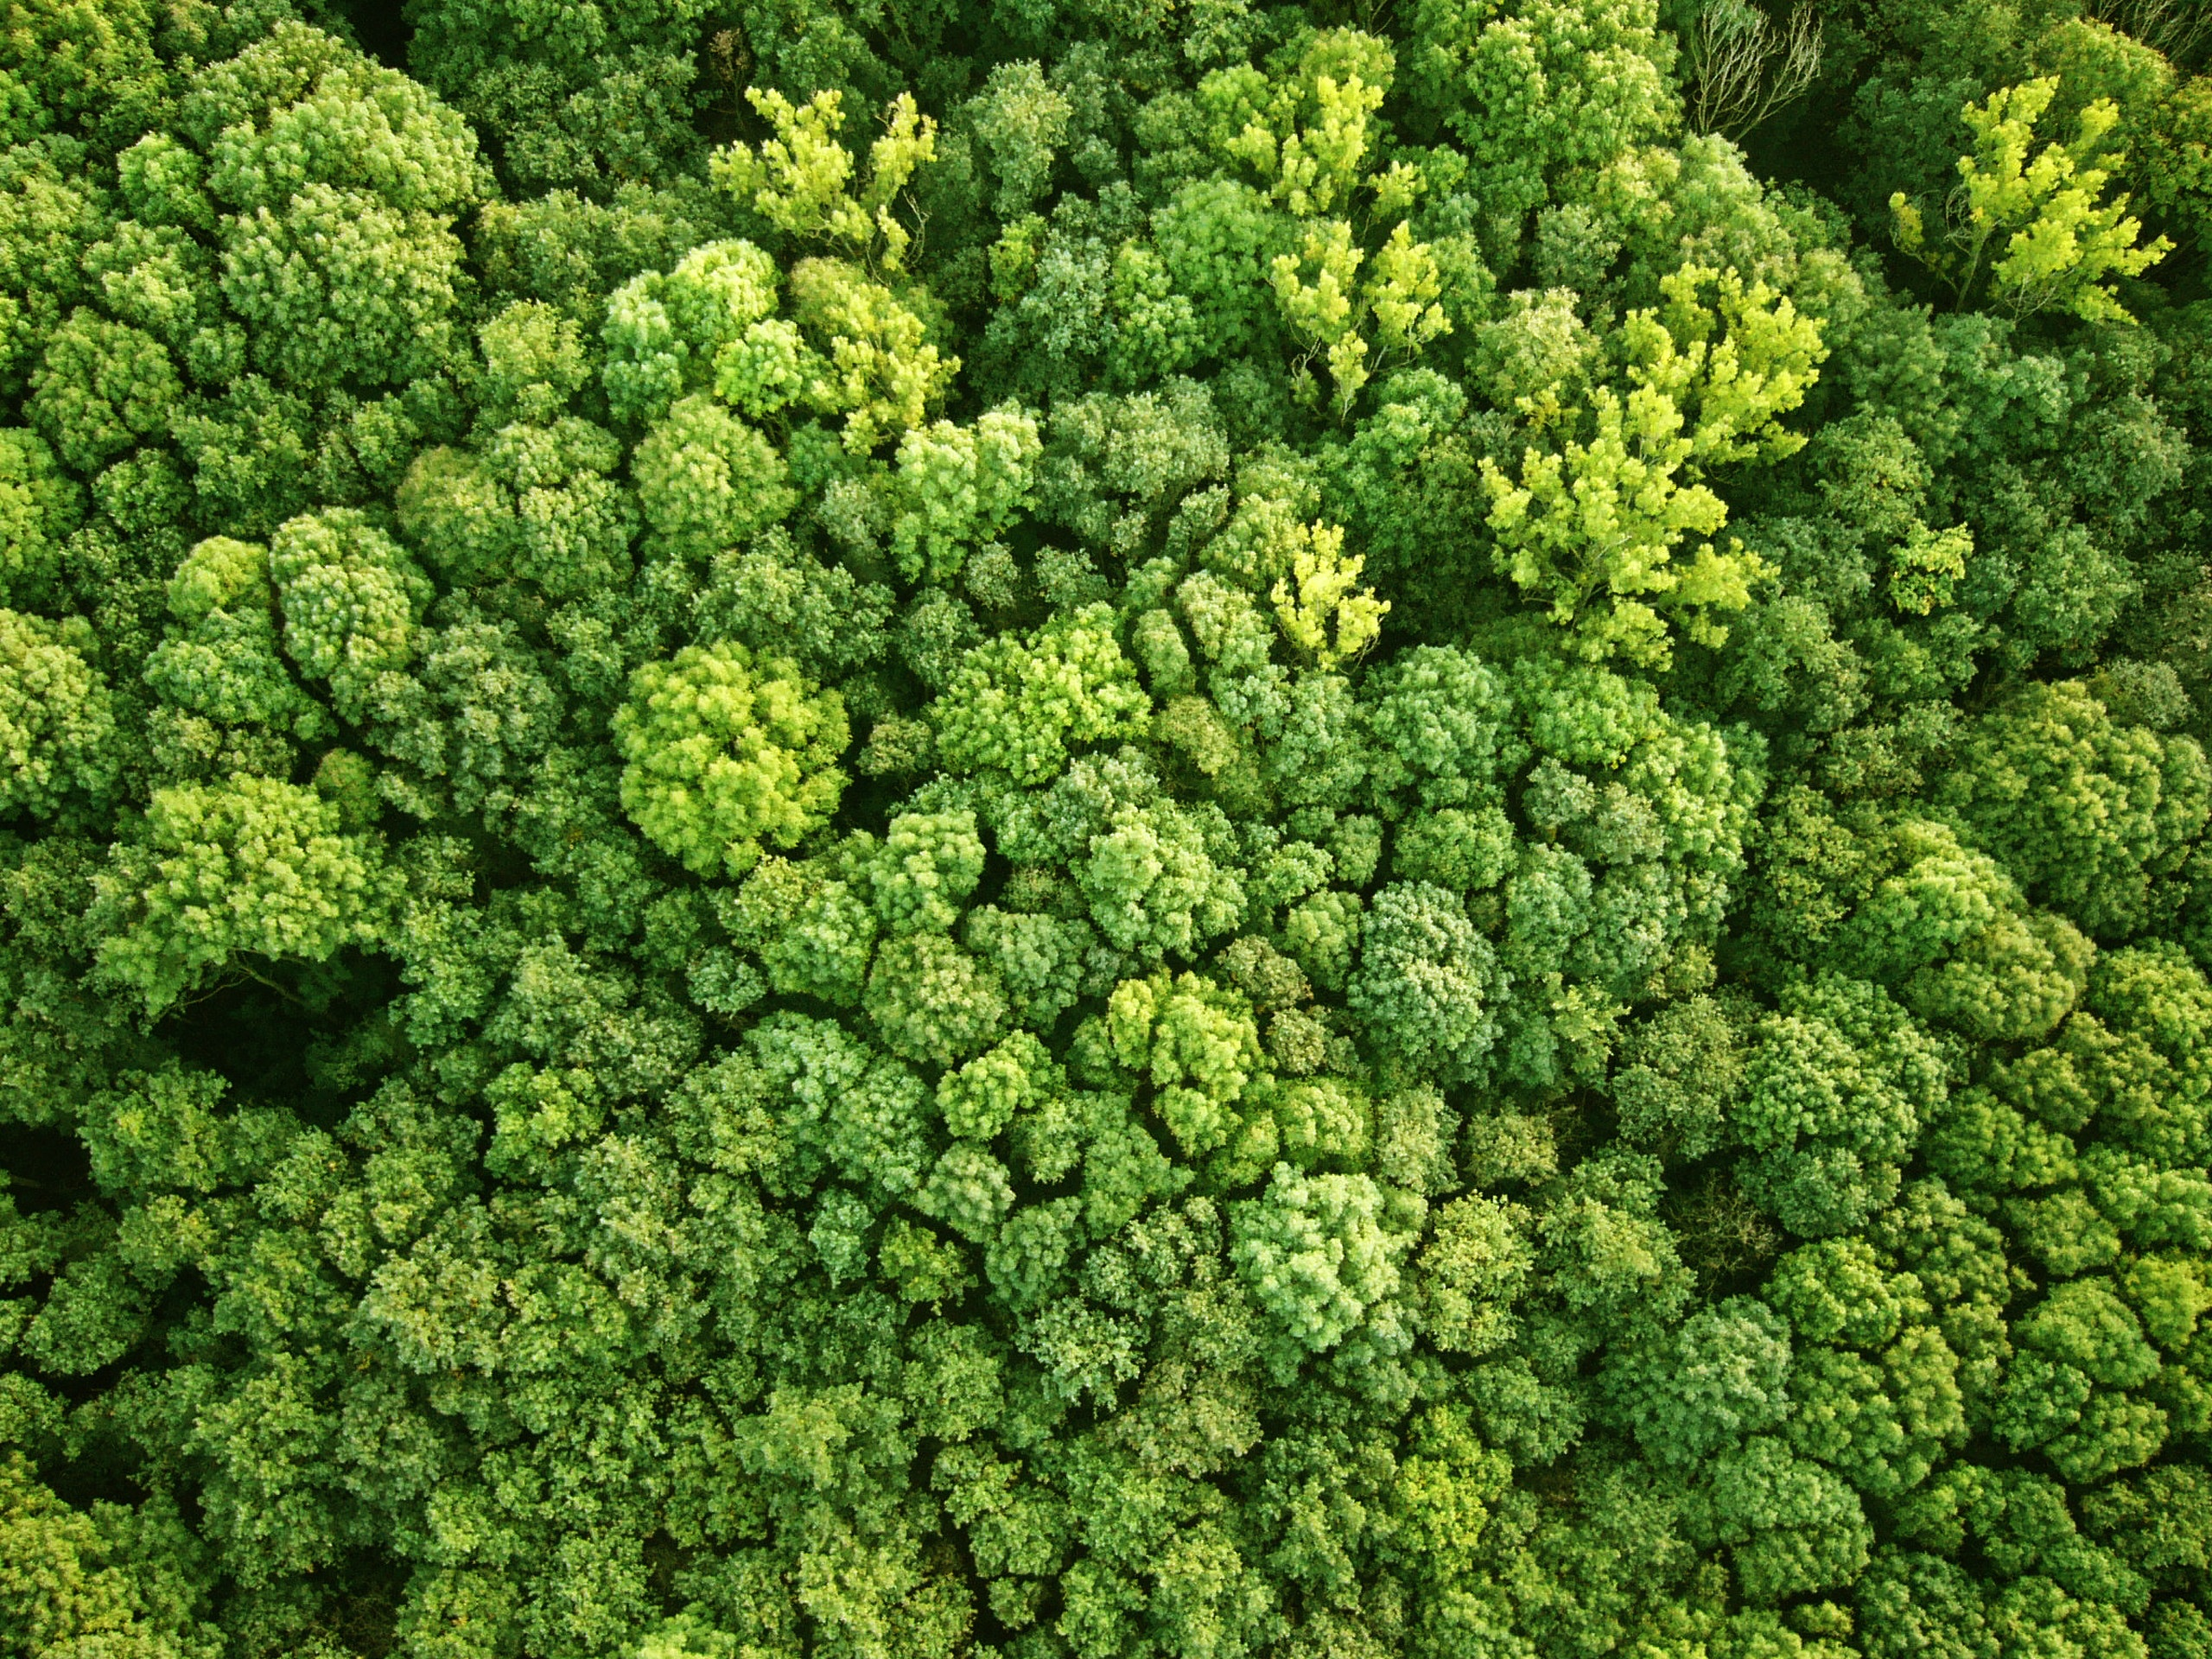
\includegraphics[keepaspectractio, width=\paperwidth]{images/forest_aerial.jpg}
        };
\end{tikzpicture}
}
\begin{frame}
  \titlepage
  \note[item]{Forests $\sim$ 80\% terrestrial biodiversity (WWF)}
  \note[item]{Soil stabilization}
  \note[item]{Forests carry out important processes: clean air and water}
  \note[item]{Forests store carbon}
\end{frame}
}

\section*{Context}

{ % all template changes are local to this group.
%%    \setbeamertemplate{navigation symbols}{}
    \begin{frame}<article:0>[plain]
      \frametitle{}
        \begin{tikzpicture}[remember picture,overlay]
            \node[at=(current page.center)] {
                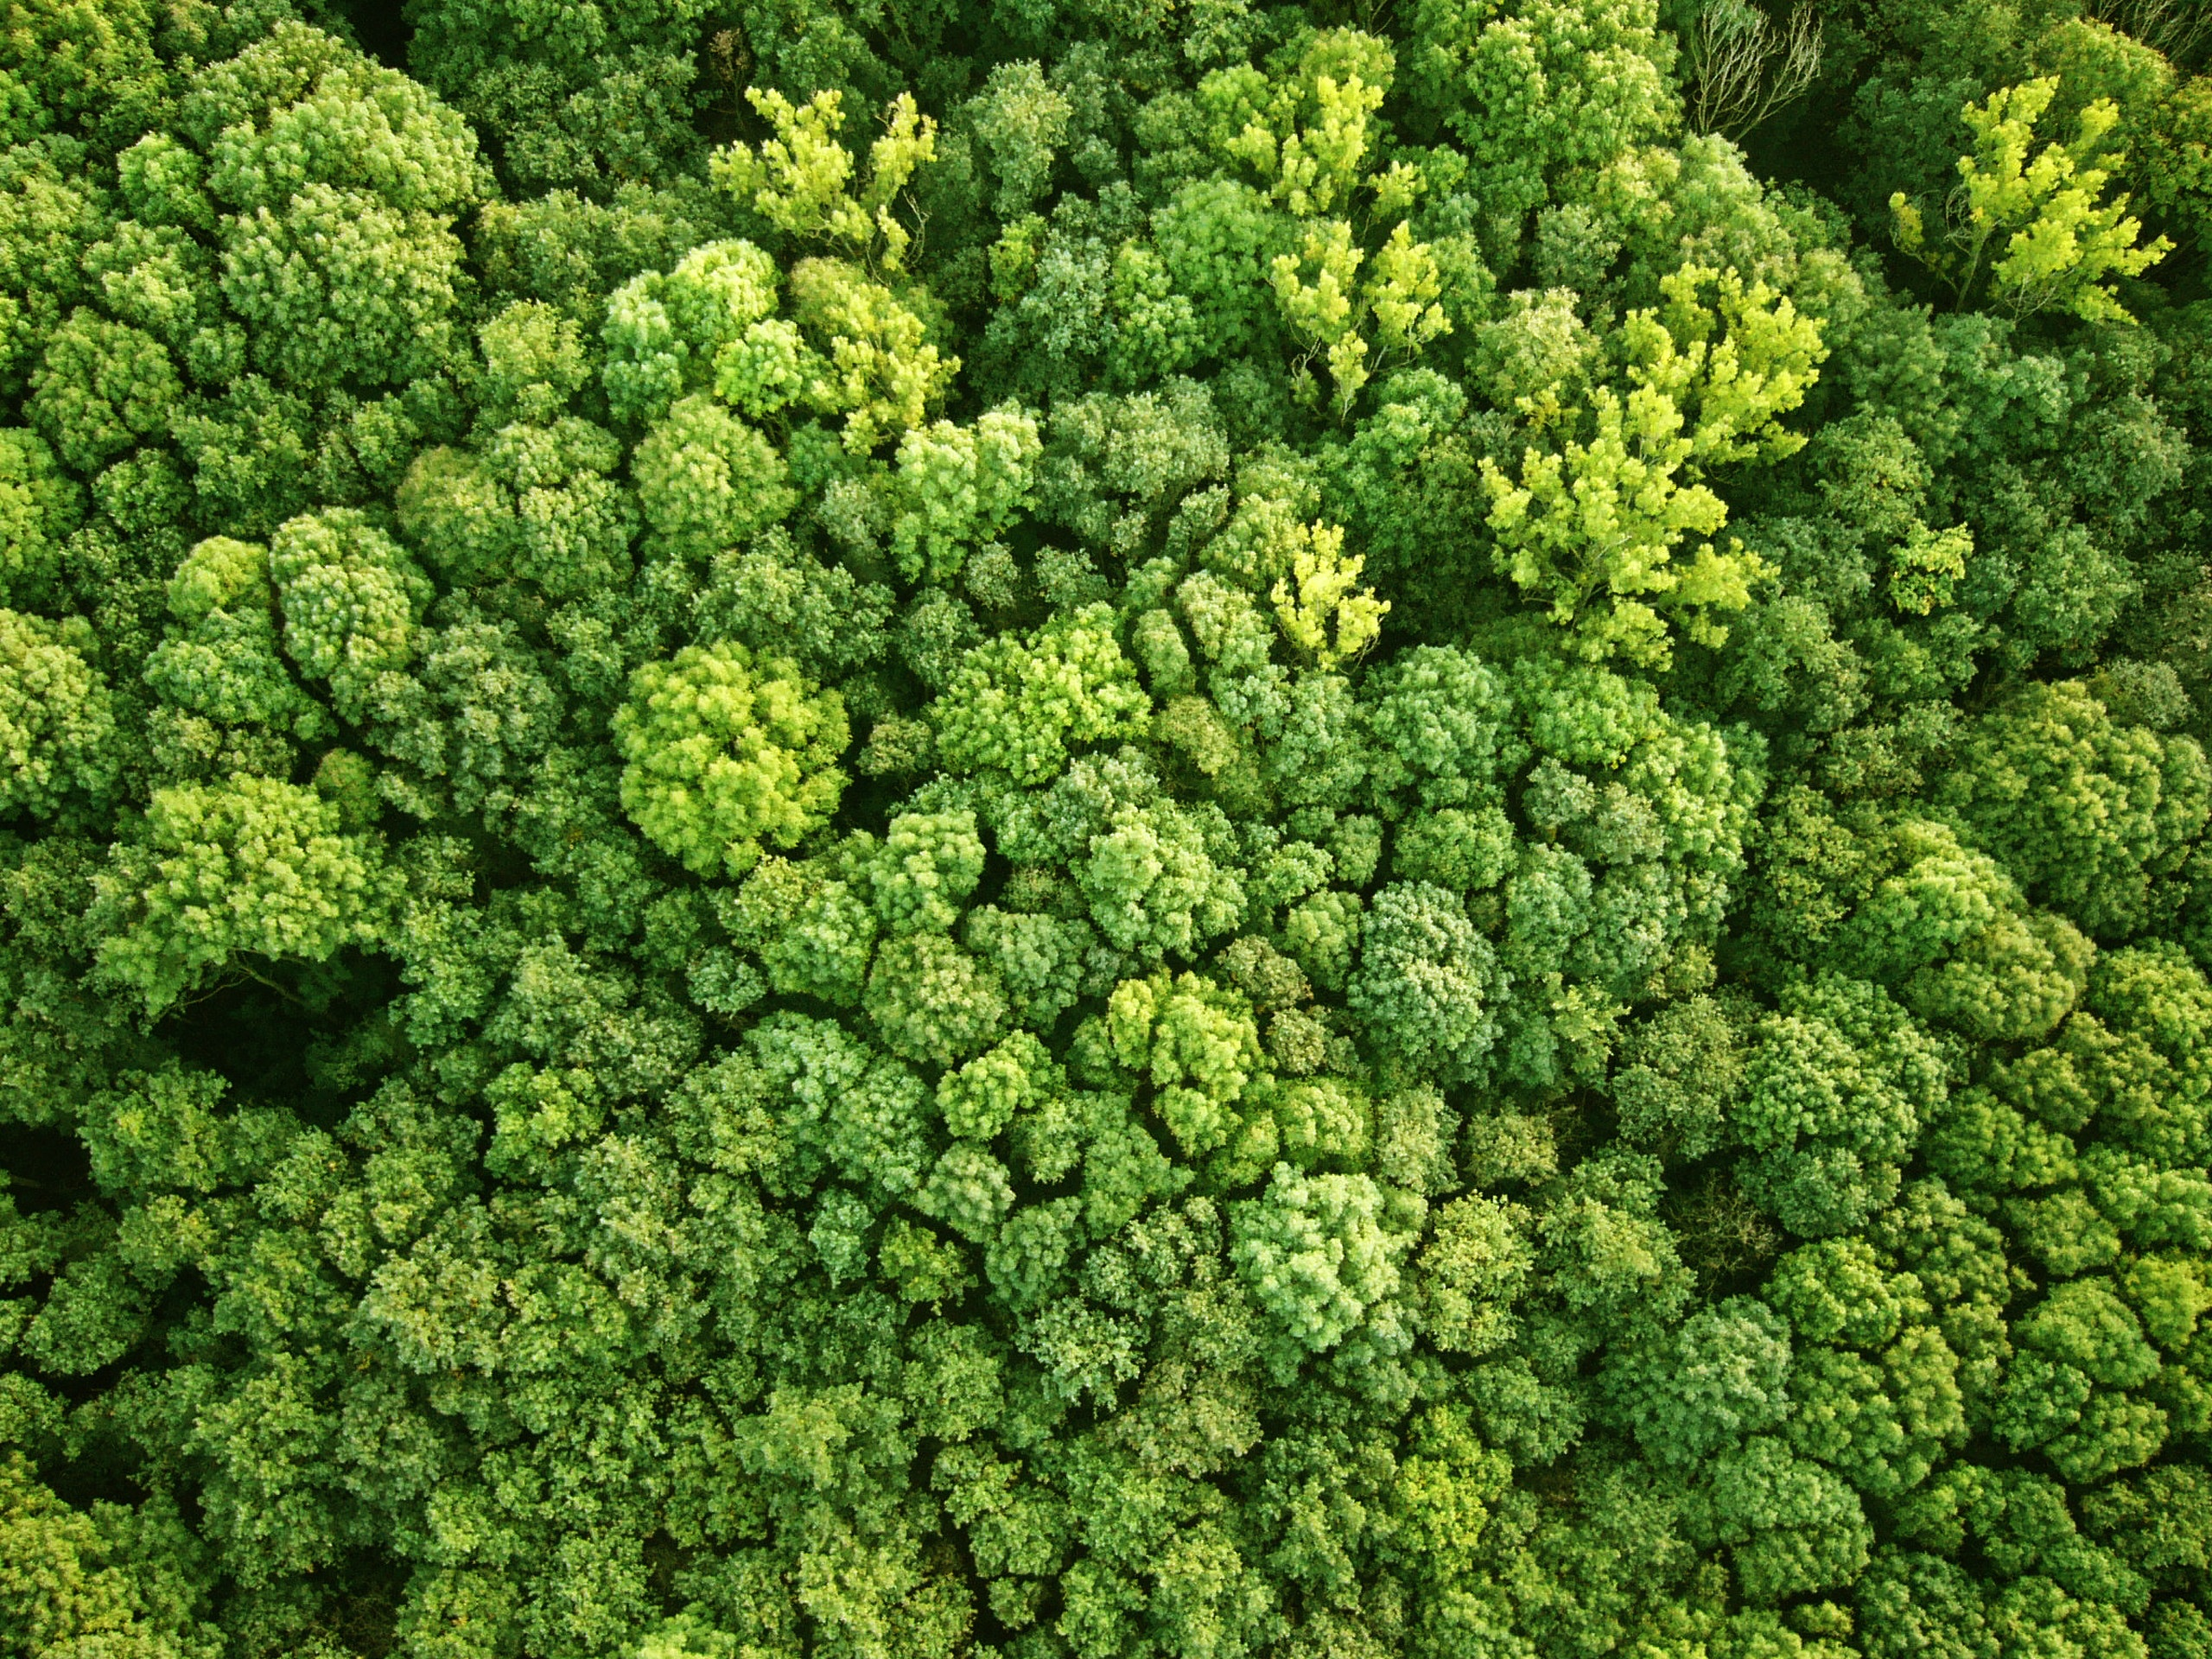
\includegraphics[keepaspectratio,
                                 width=\paperwidth]{images/forest_aerial.jpg}
            };
        \end{tikzpicture}
     \end{frame}
}

{ % all template changes are local to this group.
%%    \setbeamertemplate{navigation symbols}{}
    \begin{frame}<article:0>[plain]
      \frametitle{}
        \begin{tikzpicture}[remember picture,overlay]
            \node[at=(current page.center)] {
                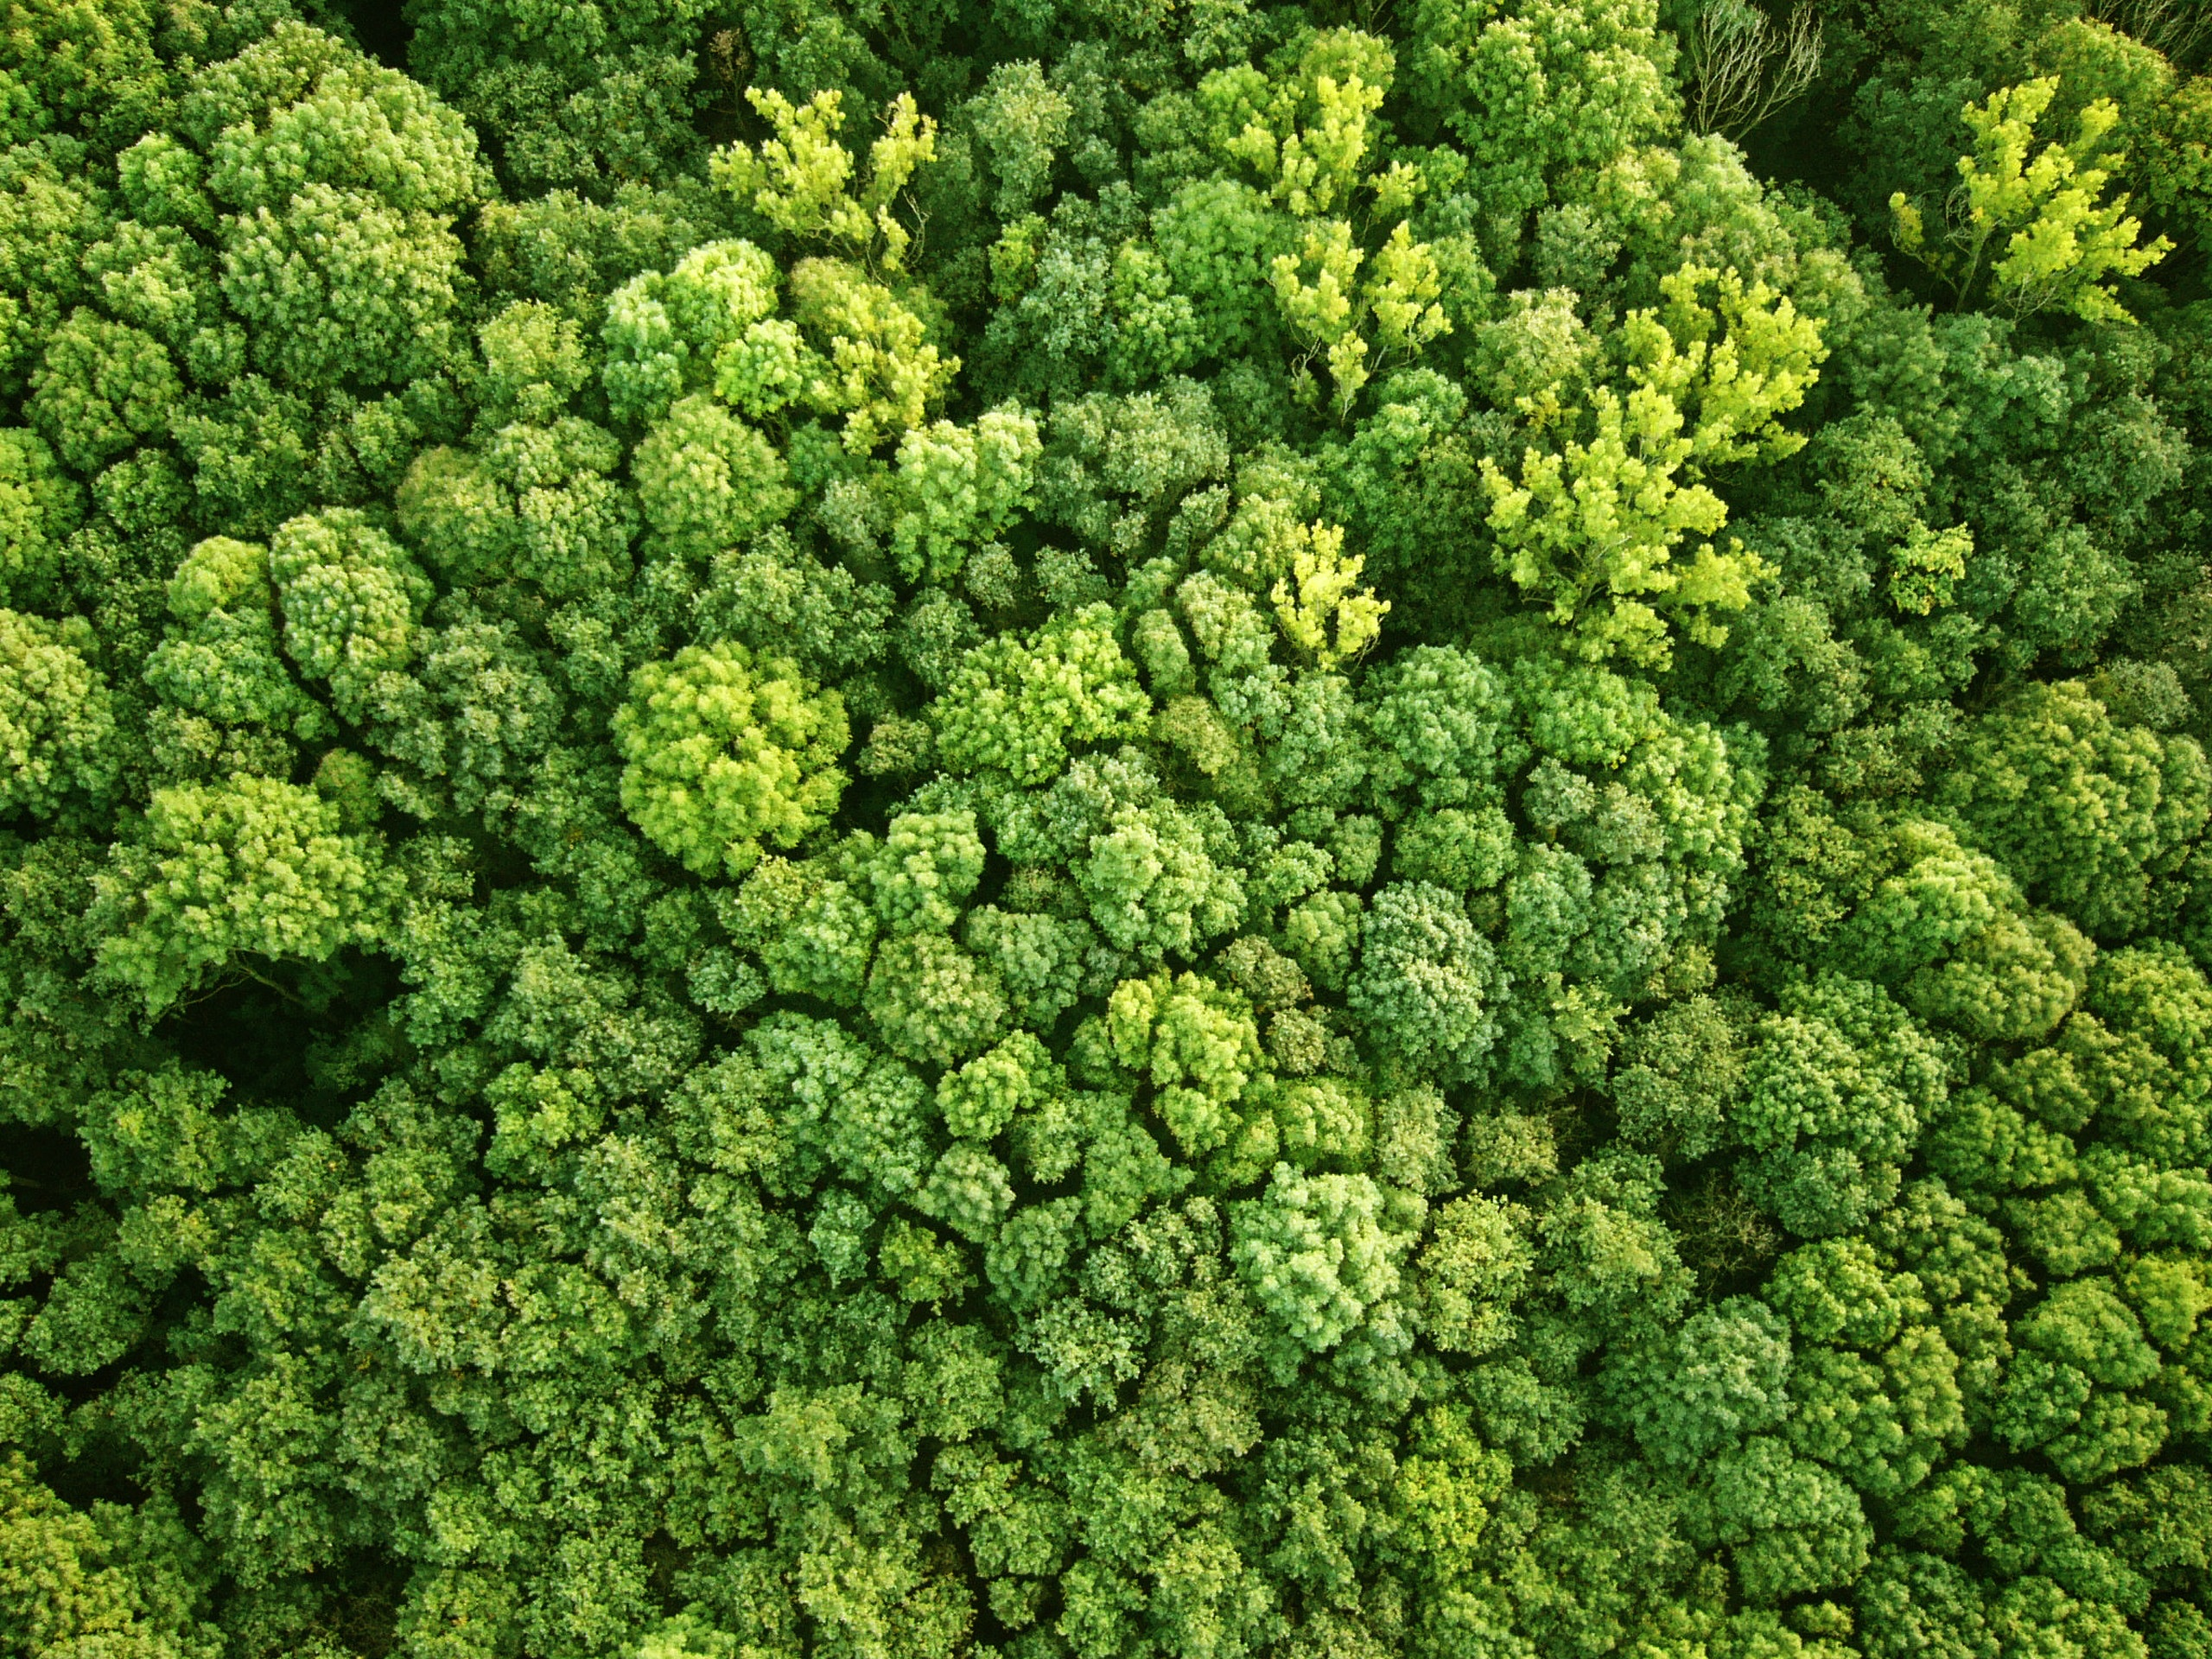
\includegraphics[keepaspectratio,
                                 width=\paperwidth]{images/forest_aerial.jpg}
            };
            \node[at=(current page.center)] {
                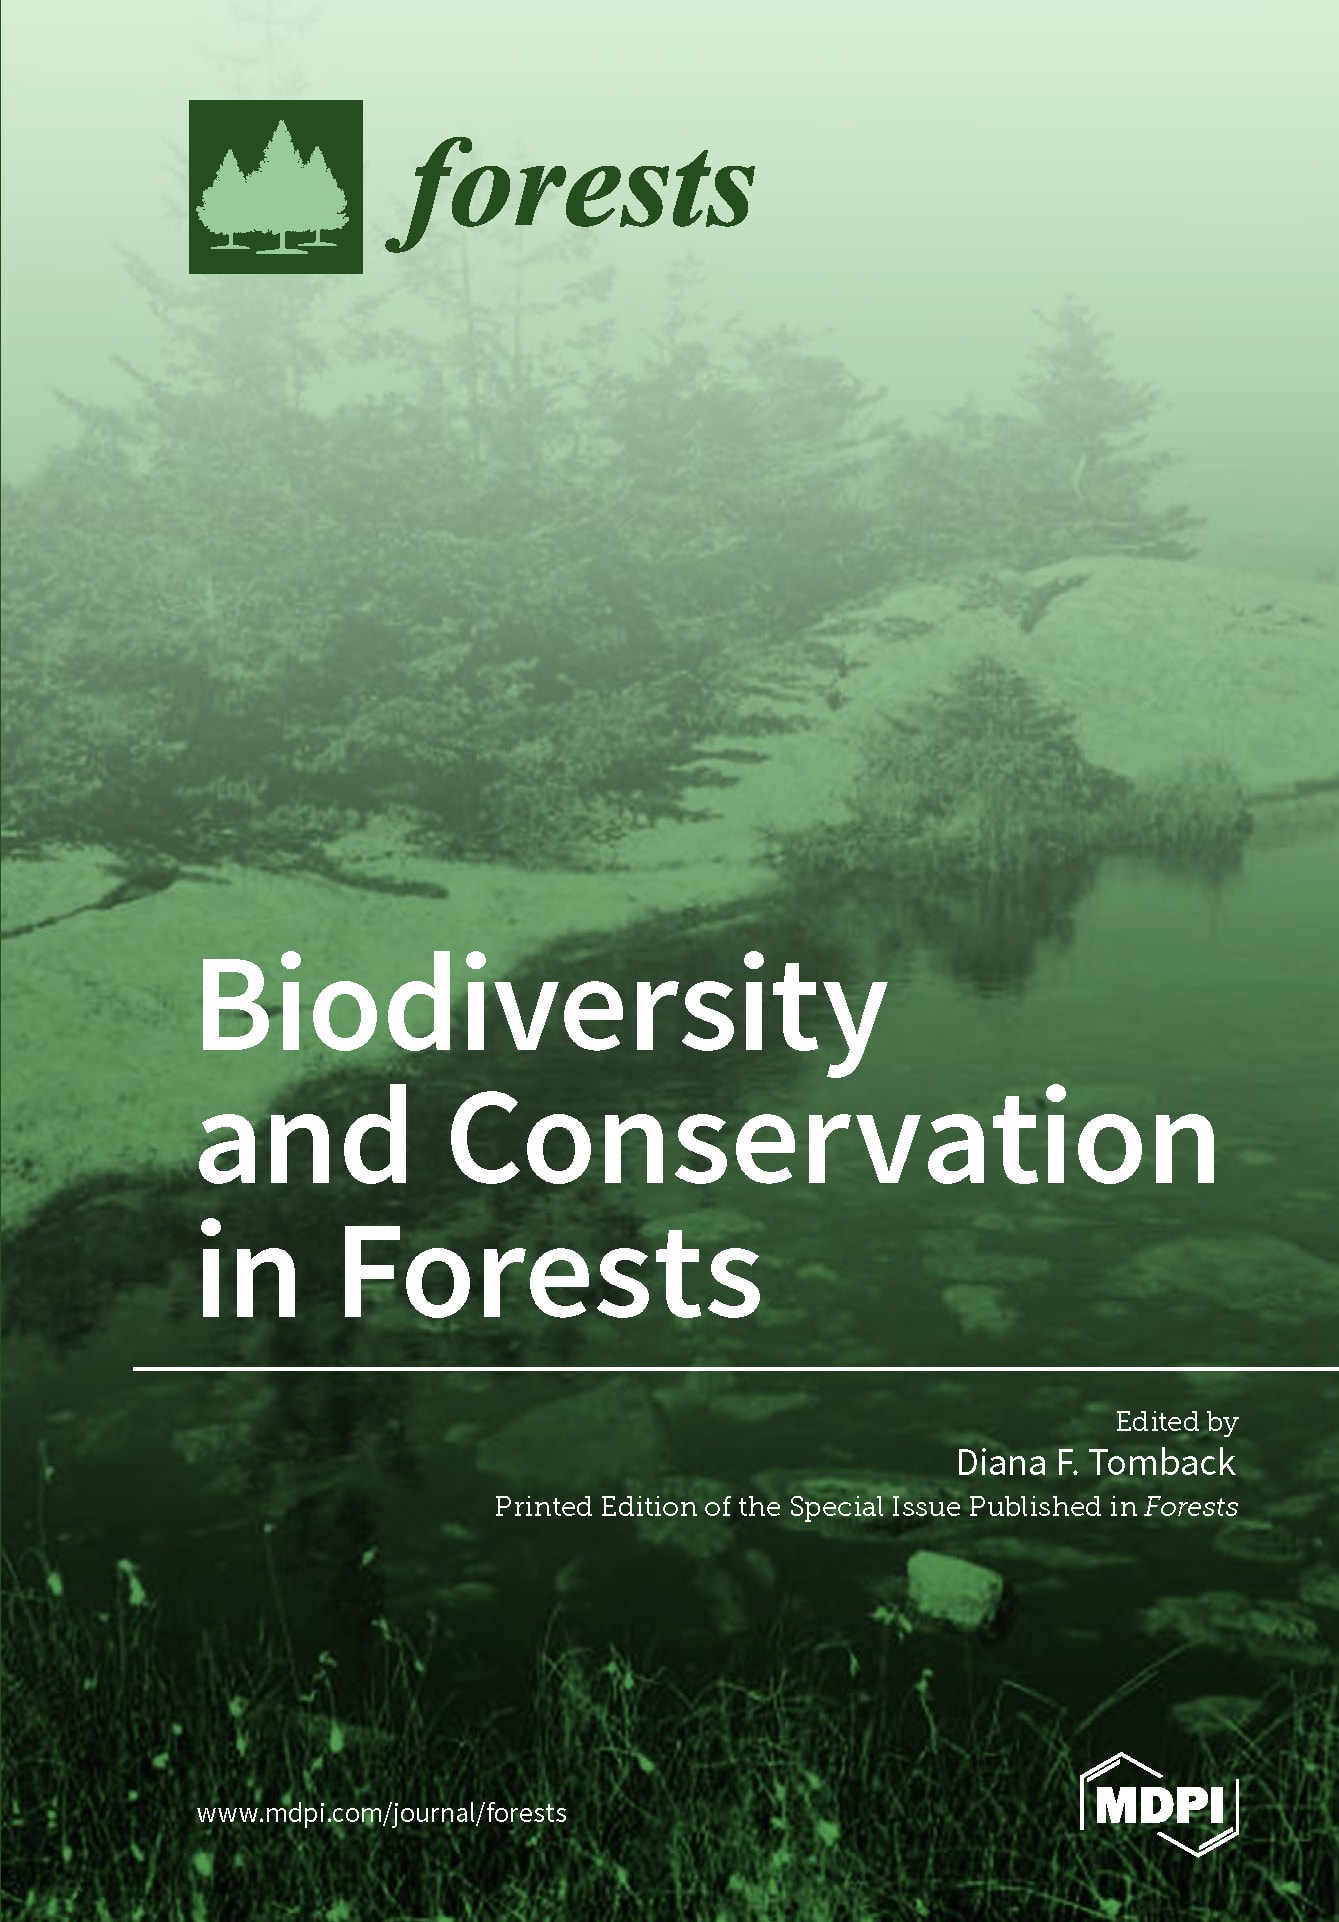
\includegraphics[keepaspectratio,
                                 height=\paperheight]{images/forest_biodiversity.jpg}
            };
        \end{tikzpicture}
     \end{frame}
}

{ % all template changes are local to this group.
%%    \setbeamertemplate{navigation symbols}{}
    \begin{frame}<article:0>[plain]
      \frametitle{}
        \begin{tikzpicture}[remember picture,overlay]
            \node[at=(current page.center)] {
                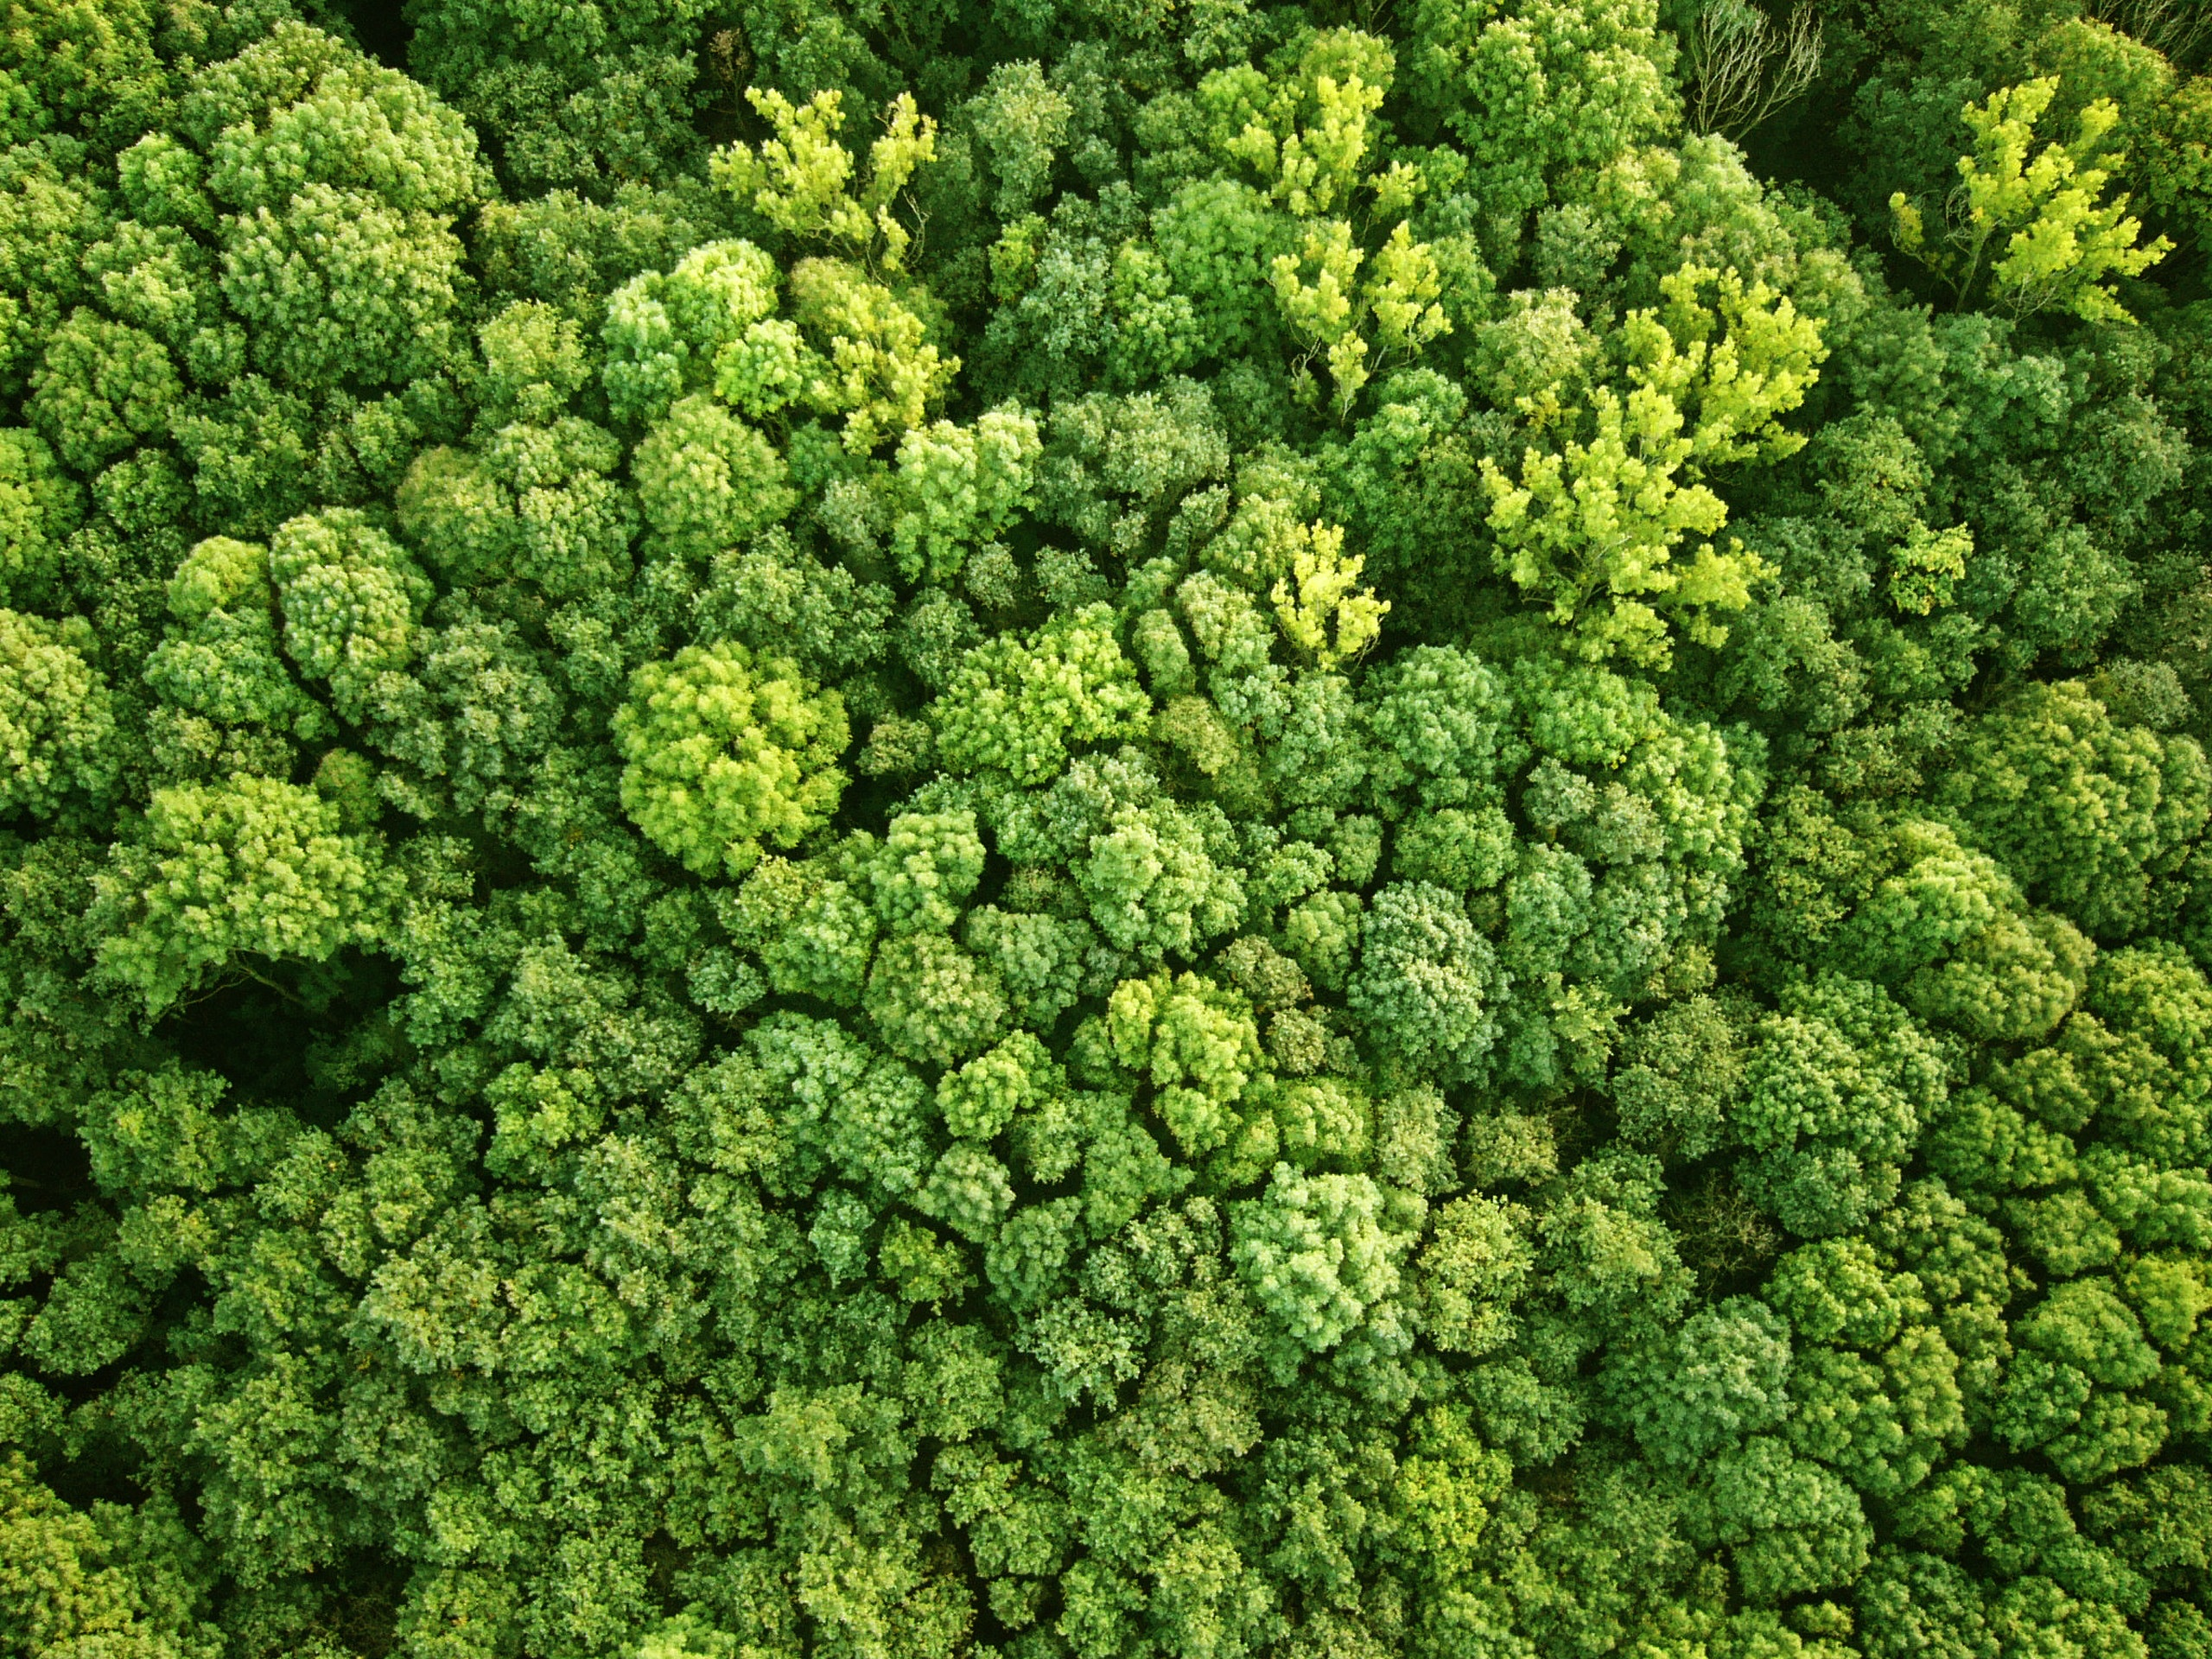
\includegraphics[keepaspectratio,
                                 width=\paperwidth]{images/forest_aerial.jpg}
            };
            \node[at=(current page.center)] {
                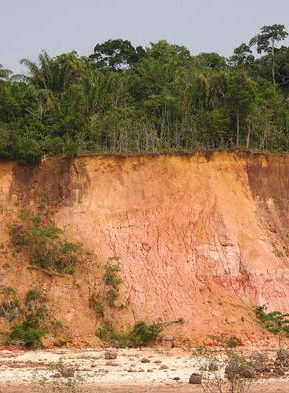
\includegraphics[keepaspectratio,
                                 height=\paperheight]{images/soil_sability.jpg}
            };
        \end{tikzpicture}
     \end{frame}
}


{ % all template changes are local to this group.
%%    \setbeamertemplate{navigation symbols}{}
    \begin{frame}<article:0>[plain]
      \frametitle{}
        \begin{tikzpicture}[remember picture,overlay]
            \node[at=(current page.center)] {
                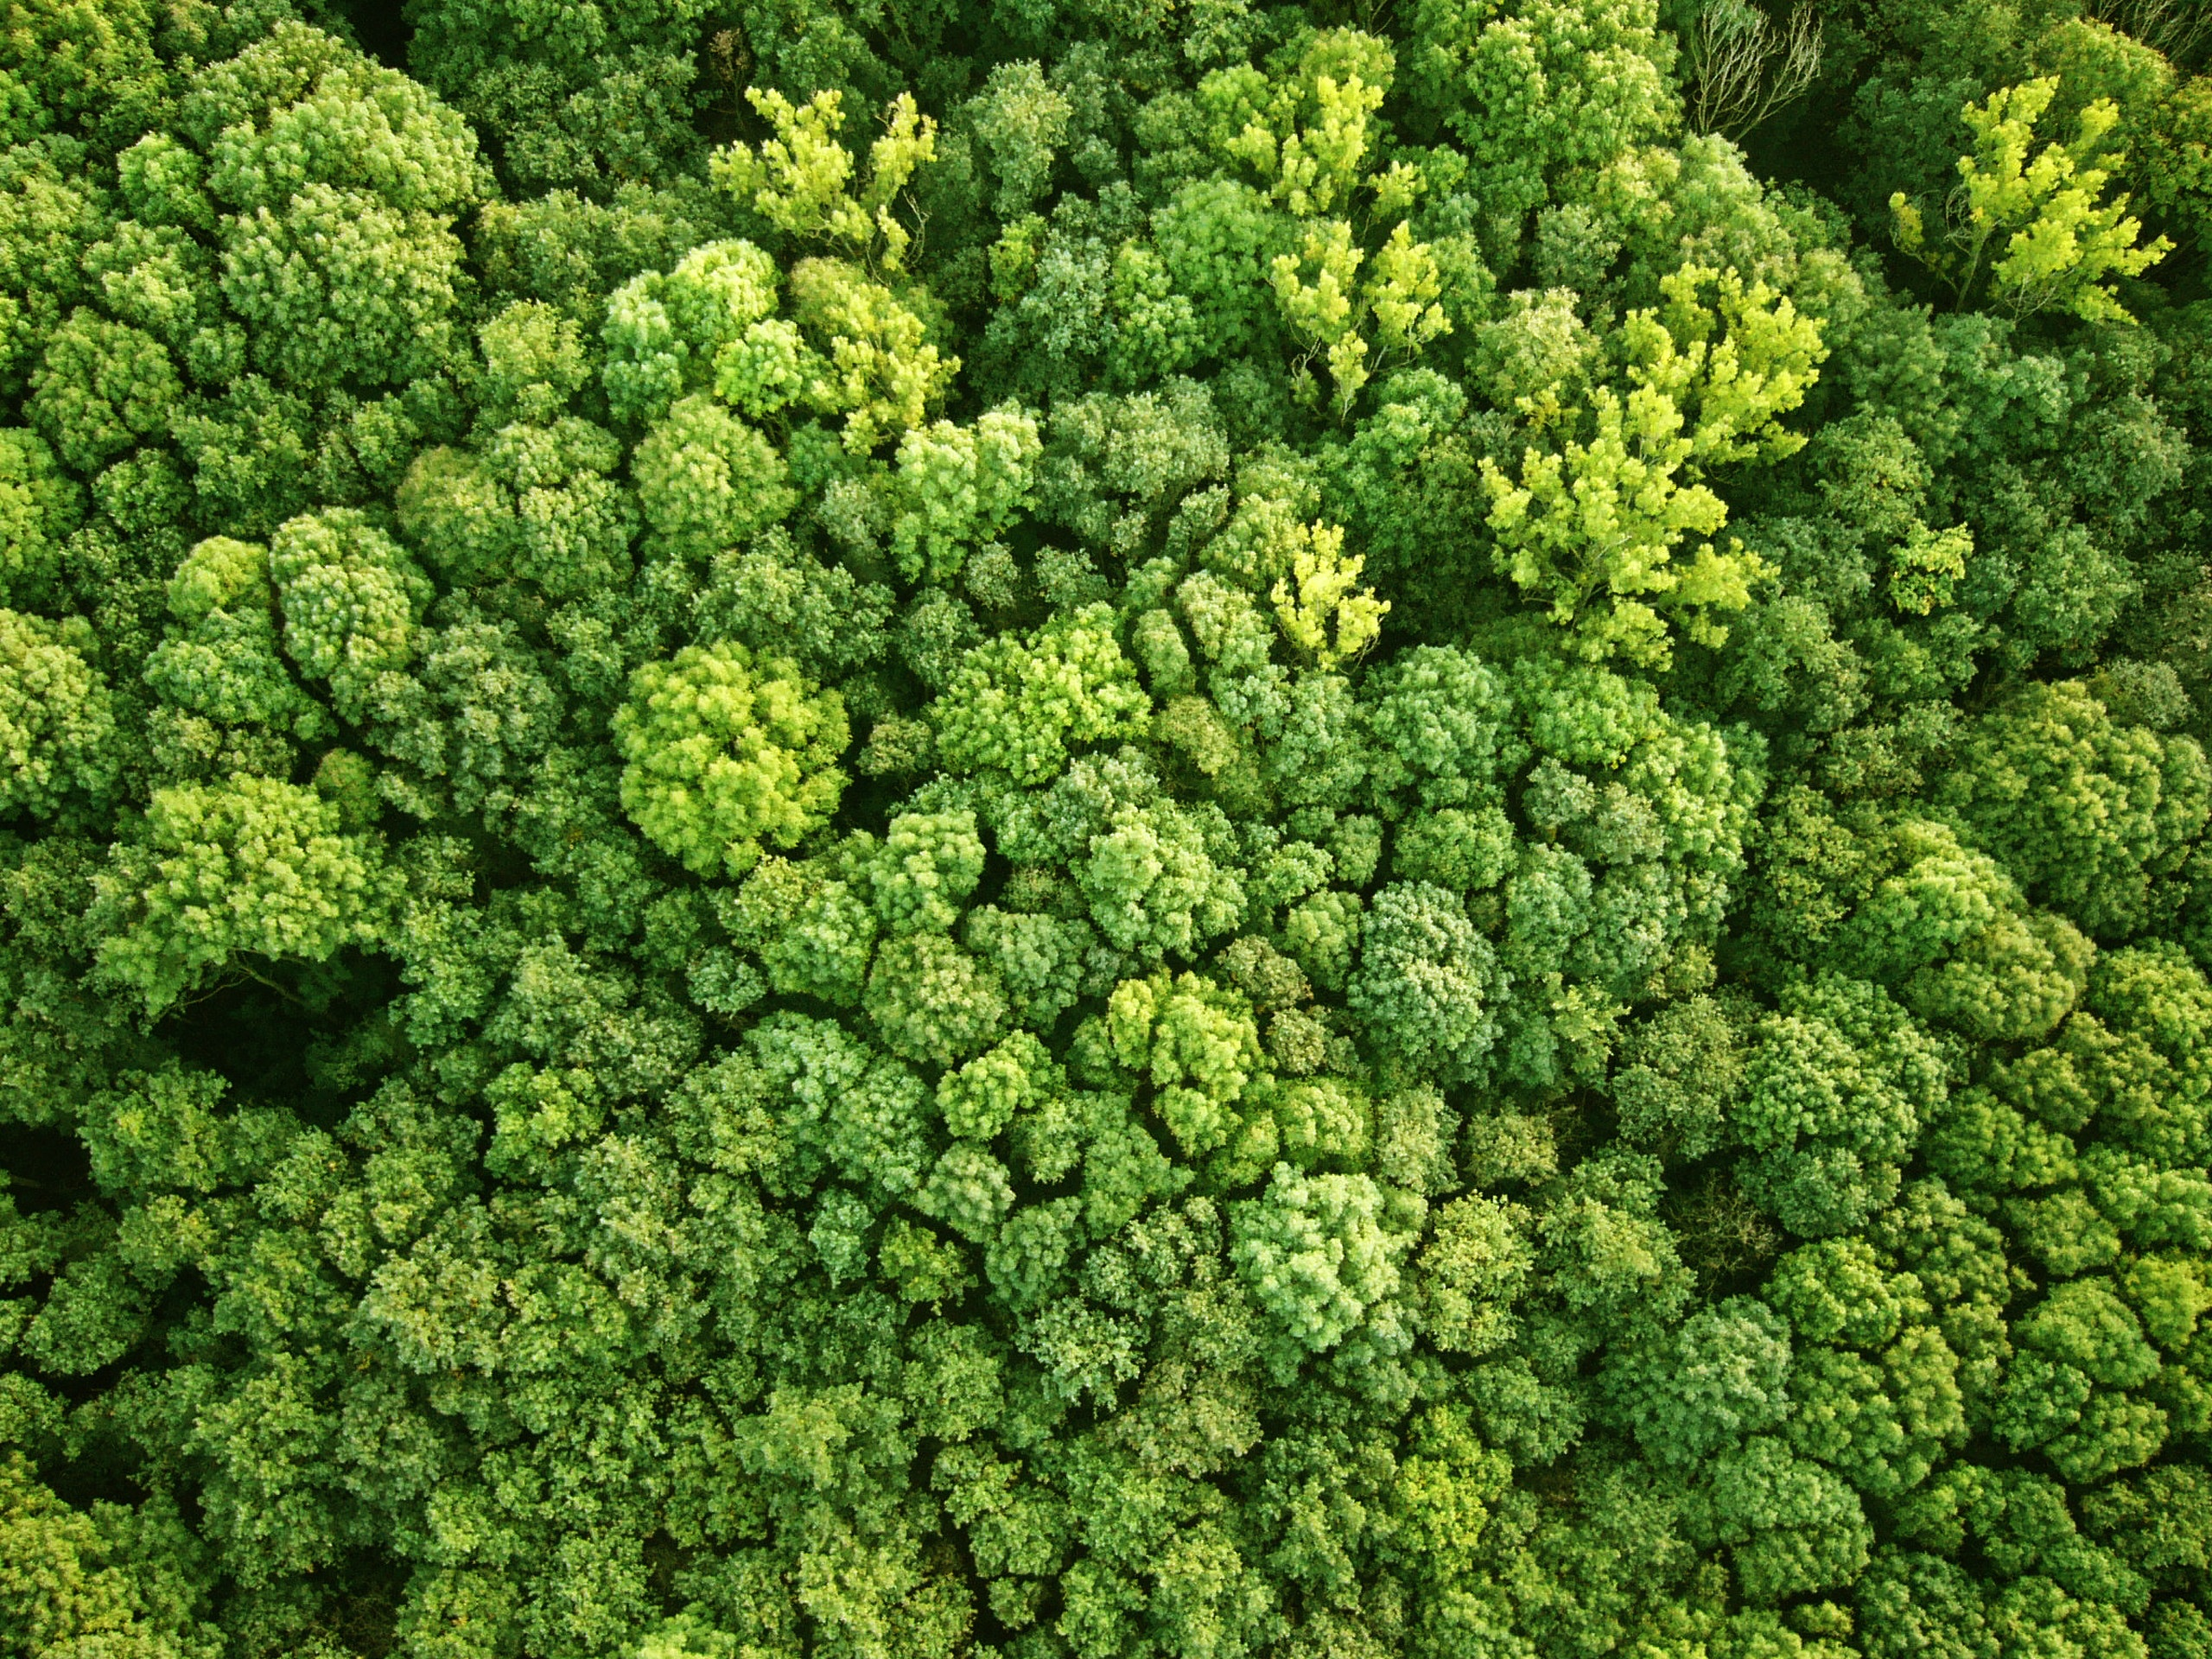
\includegraphics[keepaspectratio,
                                 width=\paperwidth]{images/forest_aerial.jpg}
            };
            \node[at=(current page.center)] {
                
\includegraphics[keepaspectratio,
                                 height=\paperheight]{images/glass-of-water.jpg}
            };
        \end{tikzpicture}
     \end{frame}
}


{ % all template changes are local to this group.
%%    \setbeamertemplate{navigation symbols}{}
    \begin{frame}<article:0>[plain]
      \frametitle{}
        \begin{tikzpicture}[remember picture,overlay]
            \node[at=(current page.center)] {
                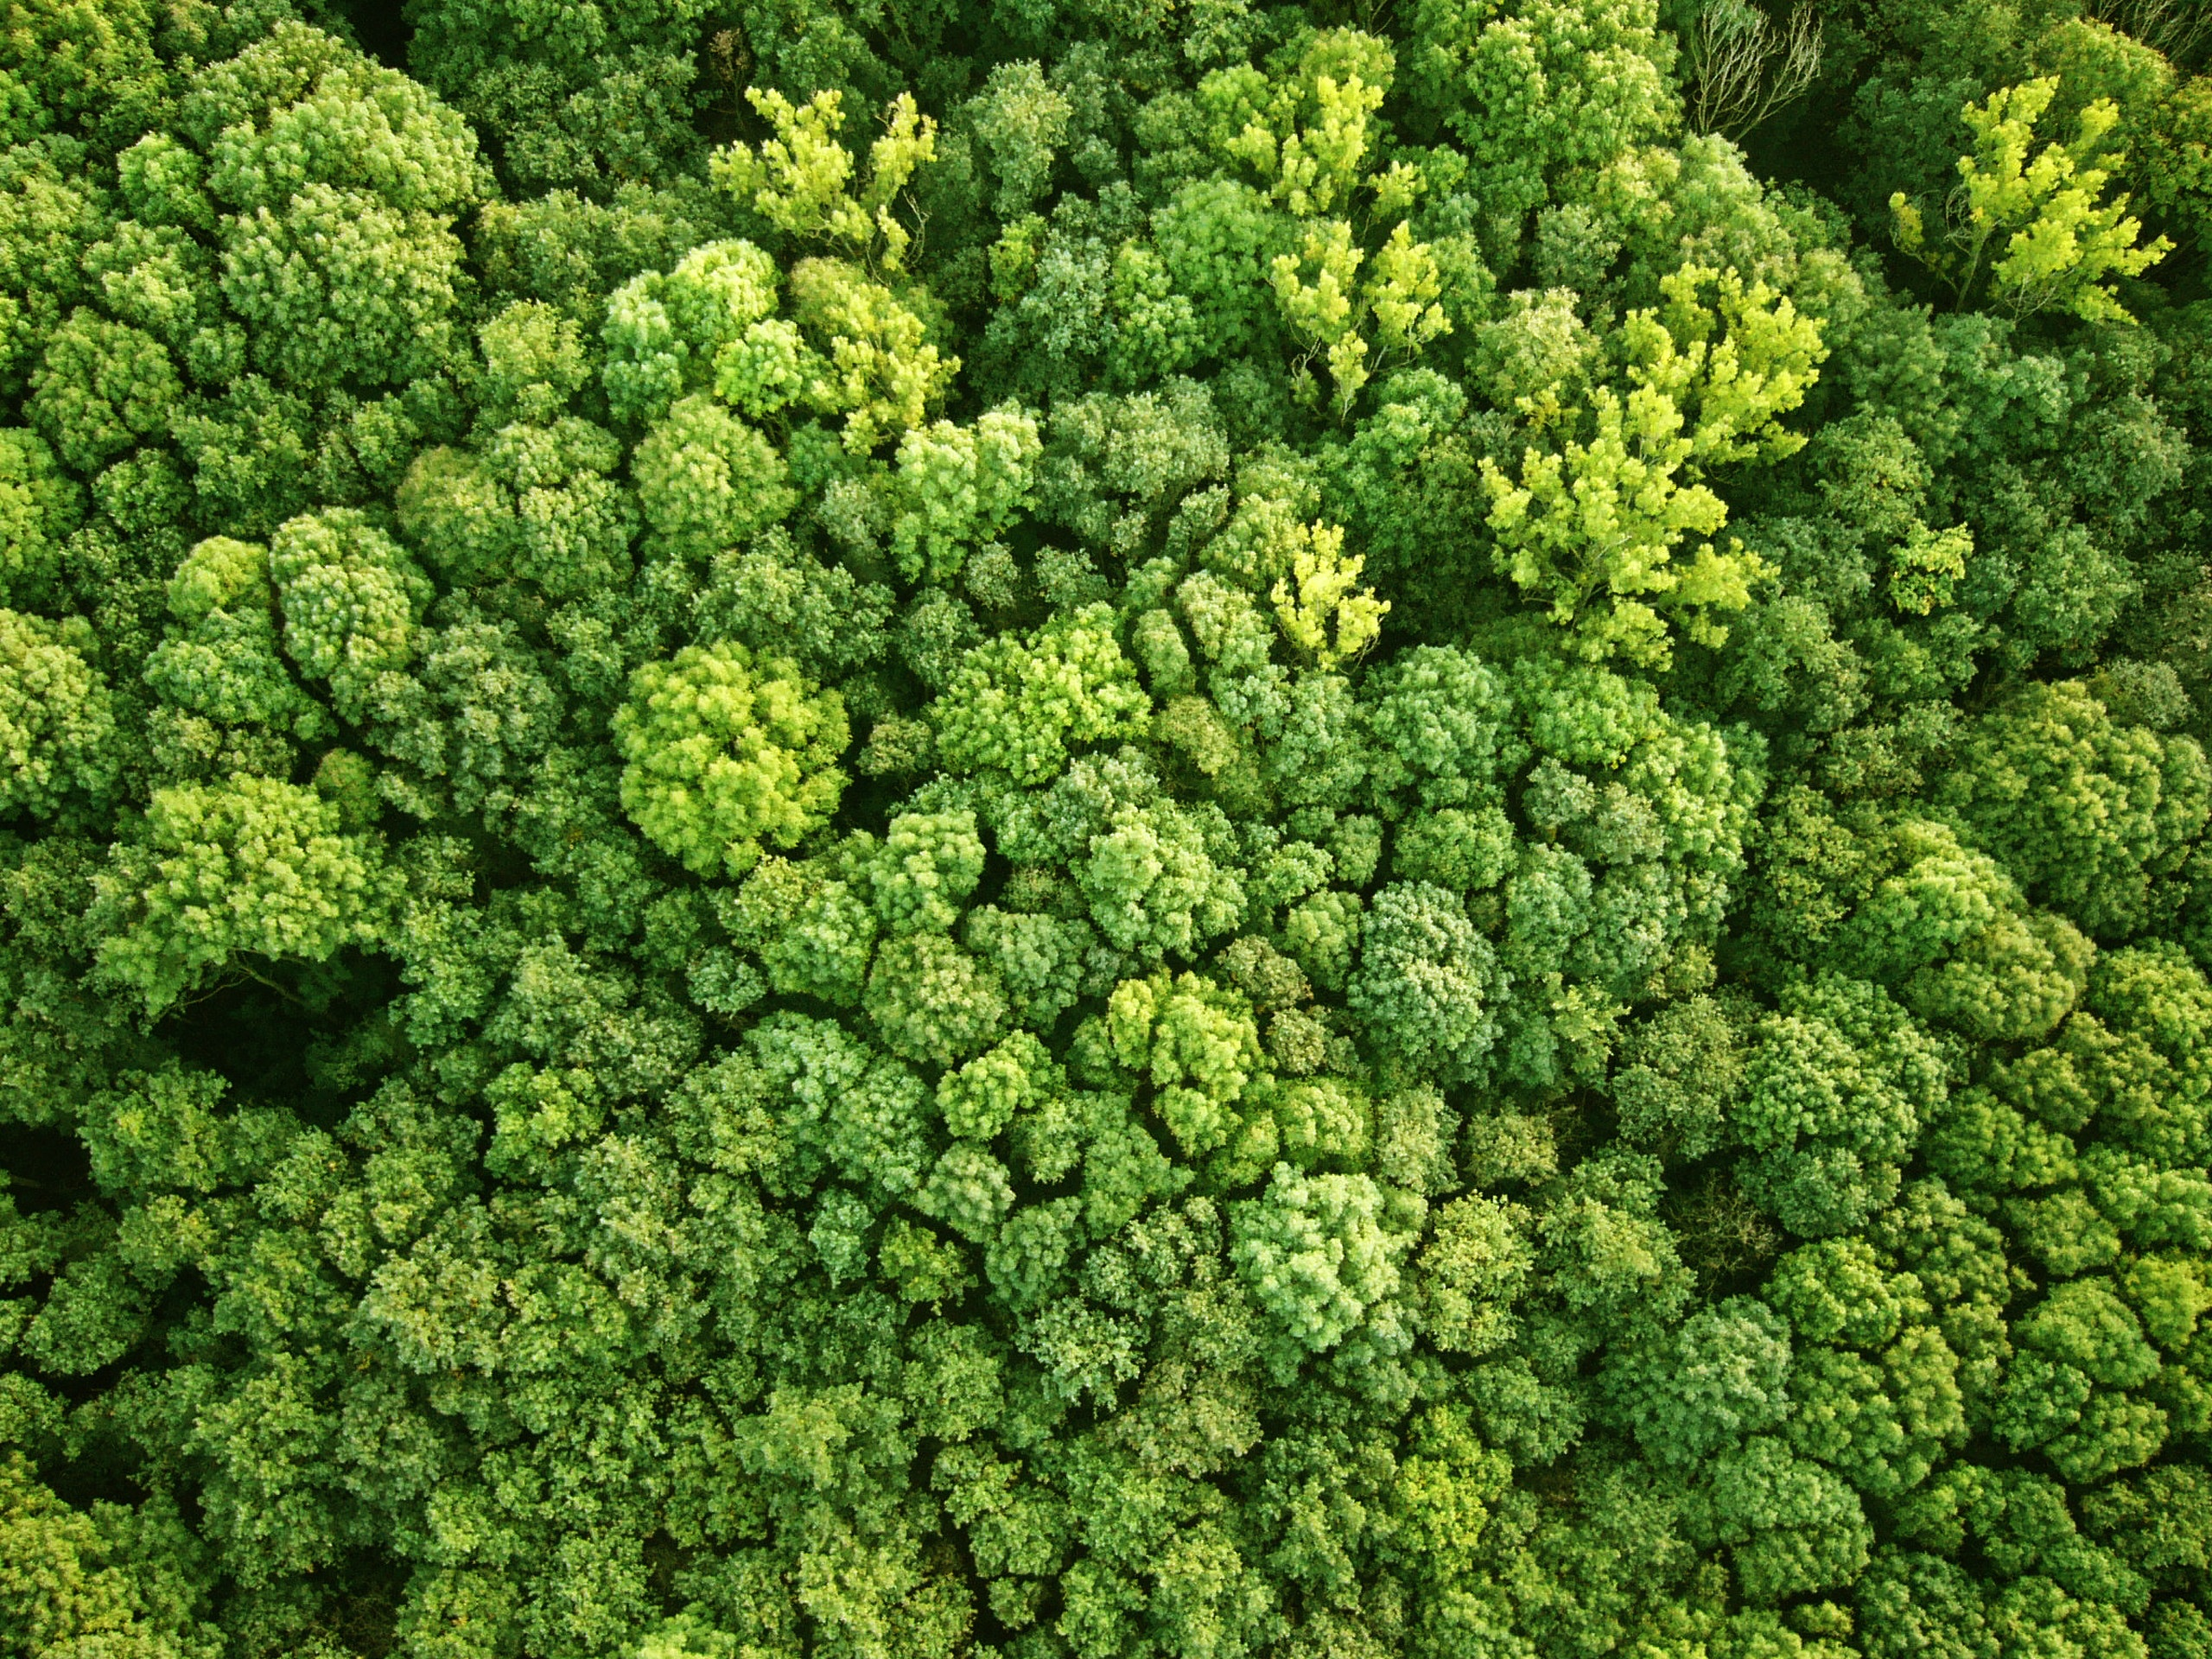
\includegraphics[keepaspectratio,
                                 width=\paperwidth]{images/forest_aerial.jpg}
            };
            \node[at=(current page.center)] {
                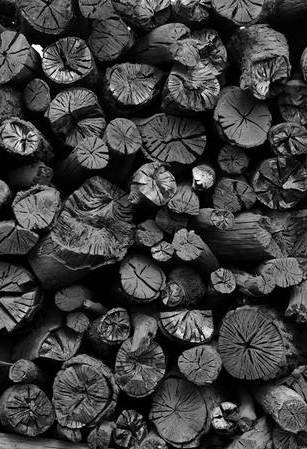
\includegraphics[keepaspectratio,
                                 height=\paperheight]{images/carbon.jpg}
            };
        \end{tikzpicture}
     \end{frame}
}


{ % all template changes are local to this group.
%%    \setbeamertemplate{navigation symbols}{}
    \begin{frame}<article:0>[plain]
      \frametitle{}
        \begin{tikzpicture}[remember picture,overlay]
            \node[at=(current page.center)] {
                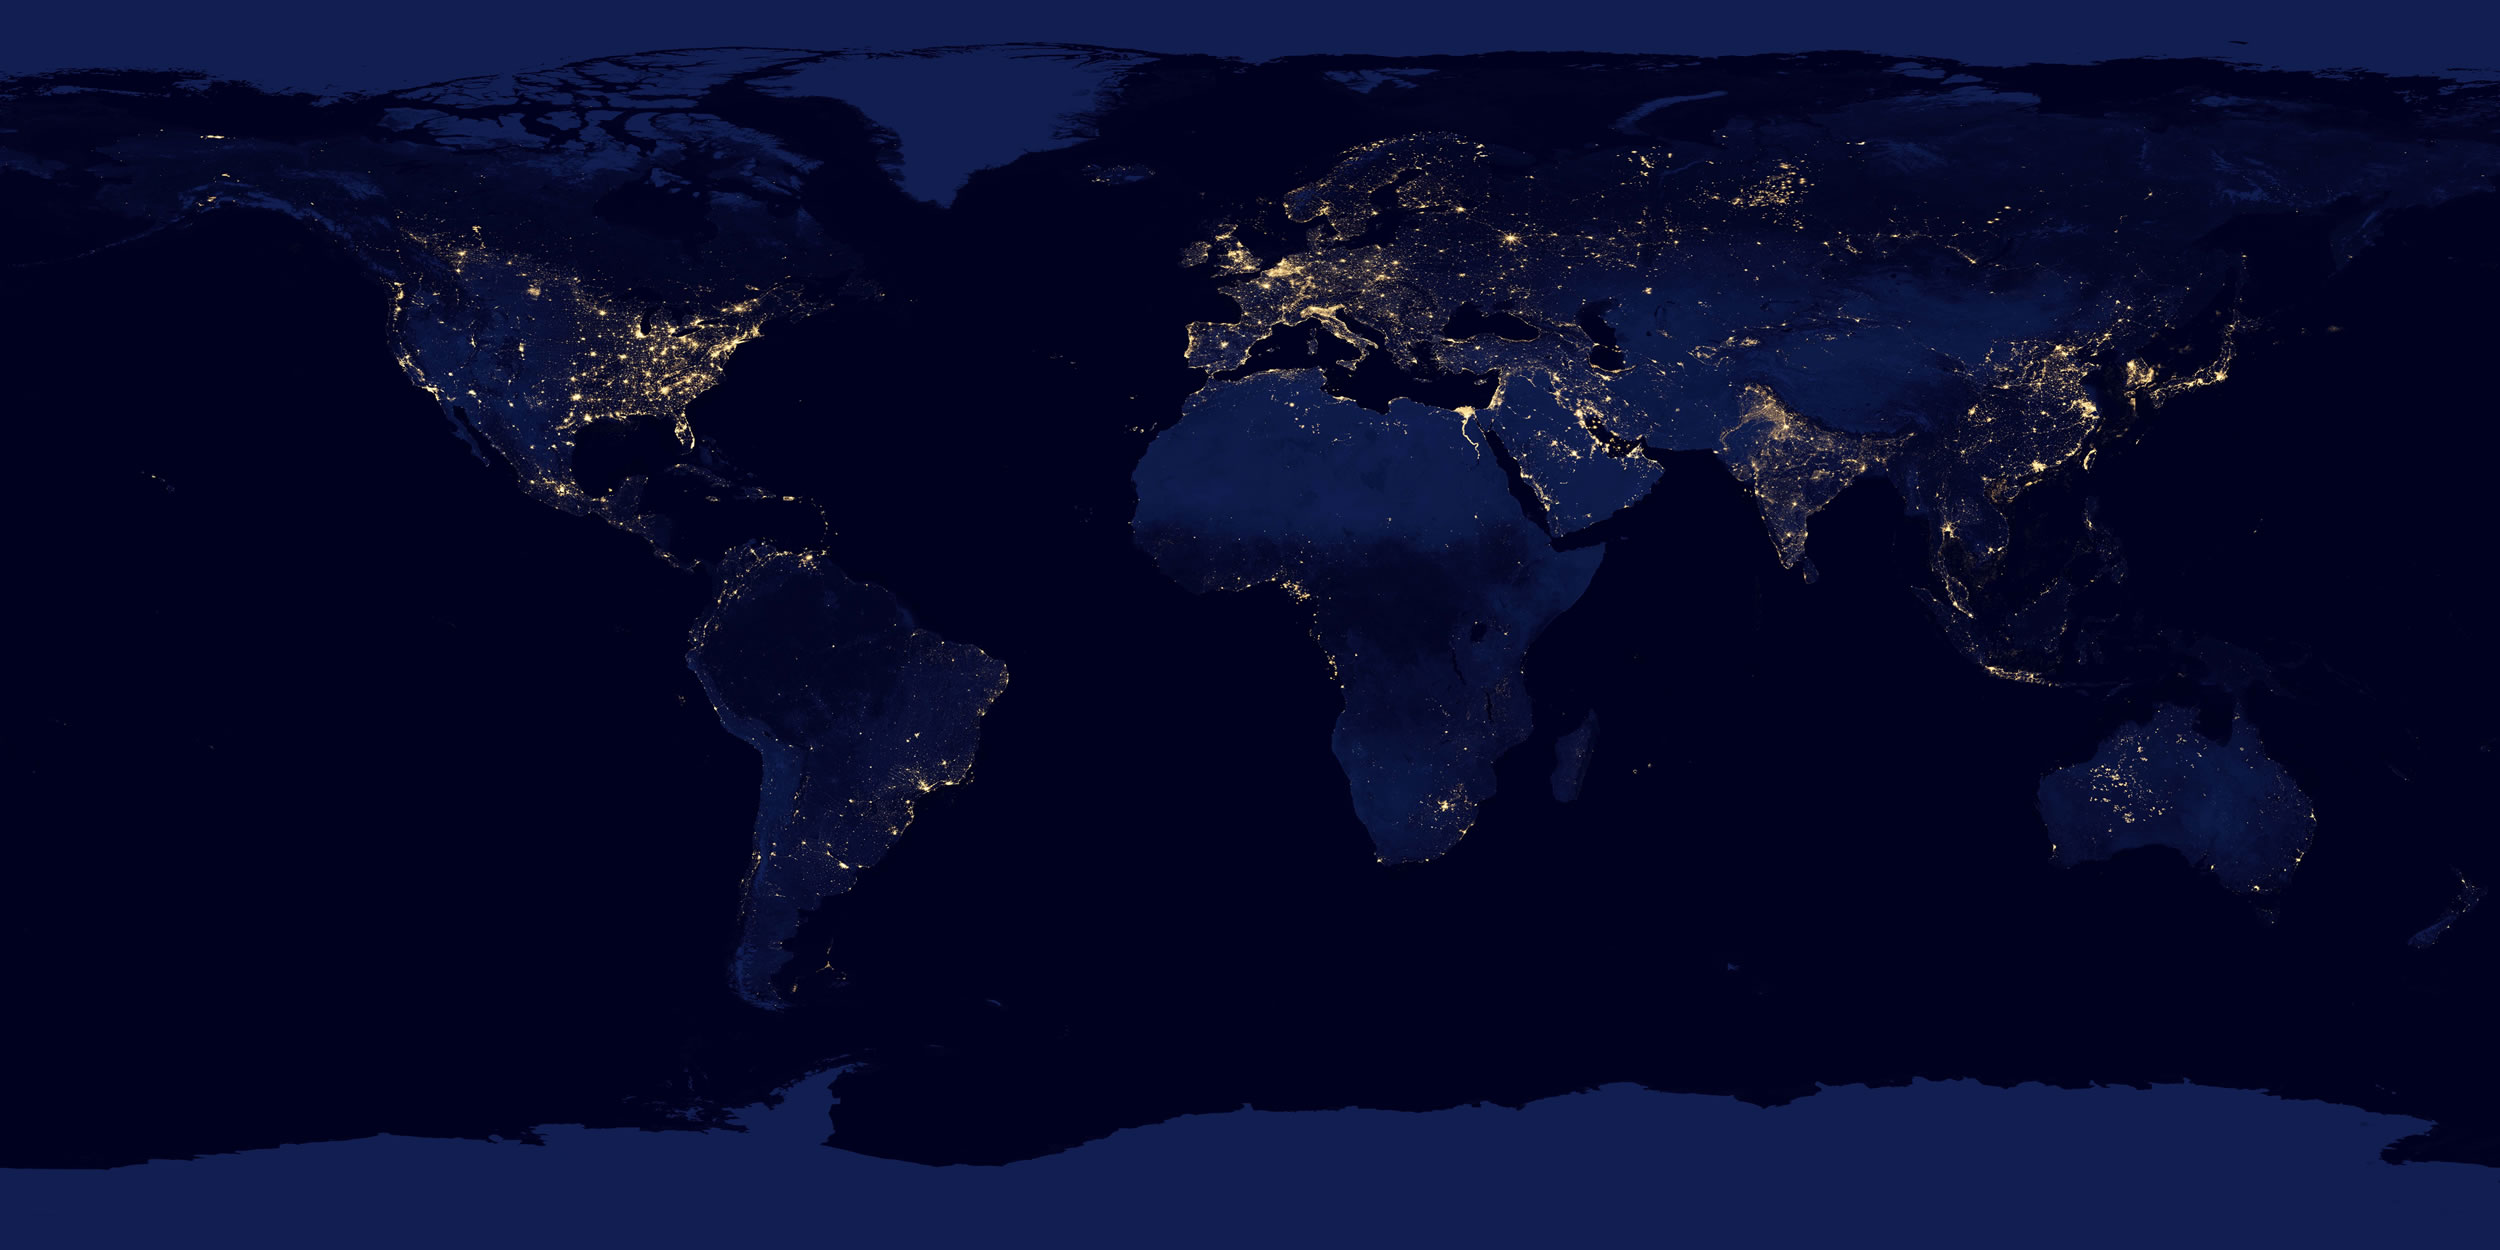
\includegraphics[keepaspectratio,
                                 height=\paperheight]{images/satellite-view-of-earth-at-night.jpg}
            };
        \end{tikzpicture}
  \note[item]{Anthropocene = proposed geological epoch distinguished by human impacts}
     \end{frame}
}



{ % all template changes are local to this group.
%%    \setbeamertemplate{navigation symbols}{}
    \begin{frame}<article:0>[plain]
      \frametitle{}
%      \cite{Ellis2020AnthropogenicCE}
        \begin{tikzpicture}[remember picture,overlay]
            \node[at=(current page.center)] {
                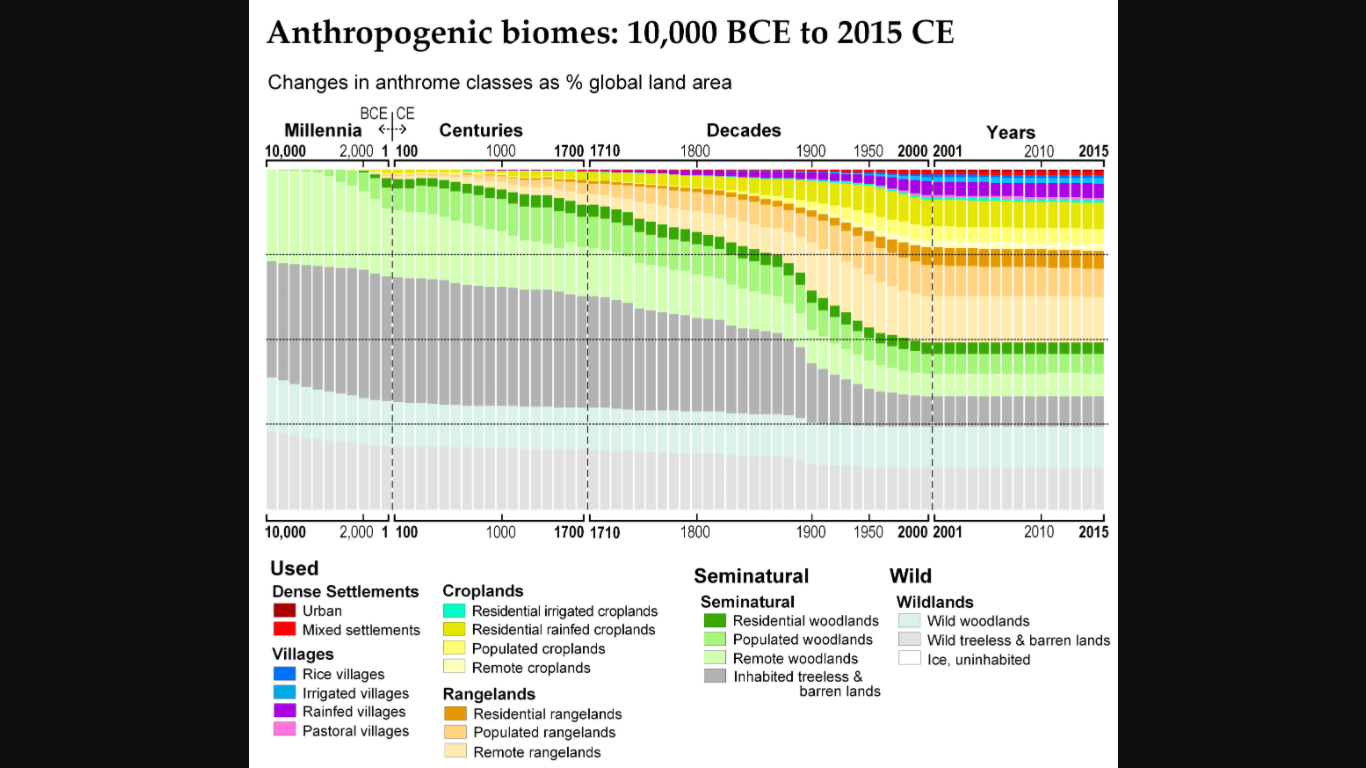
\includegraphics[keepaspectratio,
                                 width=\paperwidth,
                                 scale=0.25]{images/anthromes.png}
            };
        \end{tikzpicture}
  \note[item]{Land-use changes = conversion}
  \note[item]{One proposal is it started about 1950 with acceleration}
  \note[item]{Biodiversity changes = species introductions and extinctions}
     \end{frame}
}

{ % all template changes are local to this group.
%%    \setbeamertemplate{navigation symbols}{}
    \begin{frame}<article:0>[plain]
      \frametitle{}
        \begin{tikzpicture}[remember picture,overlay]
            \node[at=(current page.center)] {
                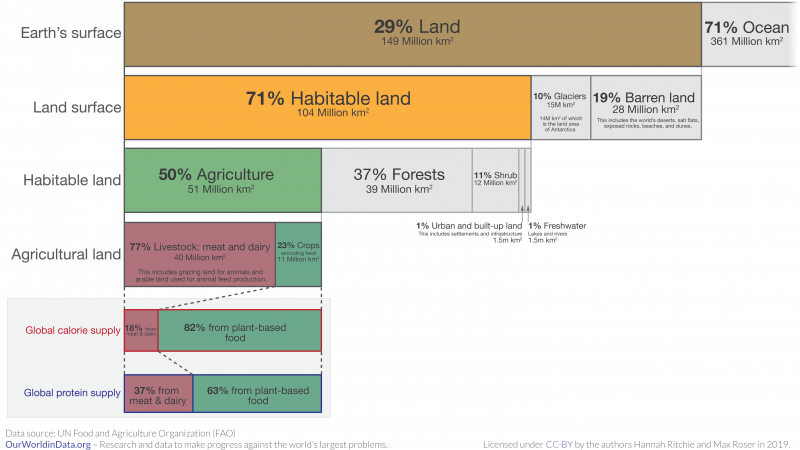
\includegraphics[keepaspectratio,
                                 width=\paperwidth,
                                 scale=0.25]{images/Global-land-use-graphic-800x506.png}
            };
        \end{tikzpicture}
  \note[item]{90\% biomass on Earth is humans and livestock}
     \end{frame}
}


{ % all template changes are local to this group.
%%    \setbeamertemplate{navigation symbols}{}
    \begin{frame}<article:0>[plain]
      \frametitle{}
        \begin{tikzpicture}[remember picture,overlay]
            \node[at=(current page.center)] {
                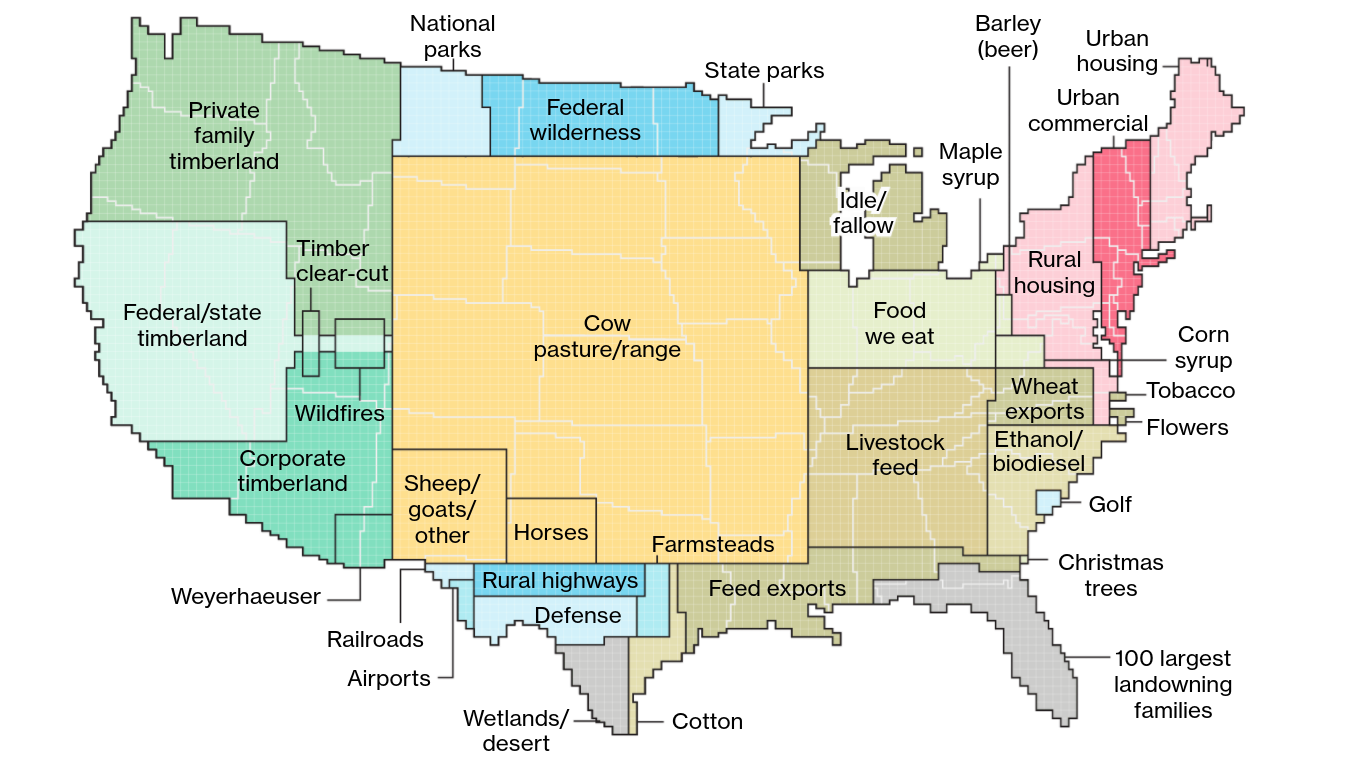
\includegraphics[keepaspectratio,
                                 width=\paperwidth]{images/how-america-uses-its-land.png}
            };
        \end{tikzpicture}
  \note[item]{90\% biomass on Earth is humans and livestock}
     \end{frame}
}




{ % all template changes are local to this group.
%%    \setbeamertemplate{navigation symbols}{}
    \begin{frame}<article:0>[plain]
      \frametitle{}
        \begin{tikzpicture}[remember picture,overlay]
            \node[at=(current page.center)] {
                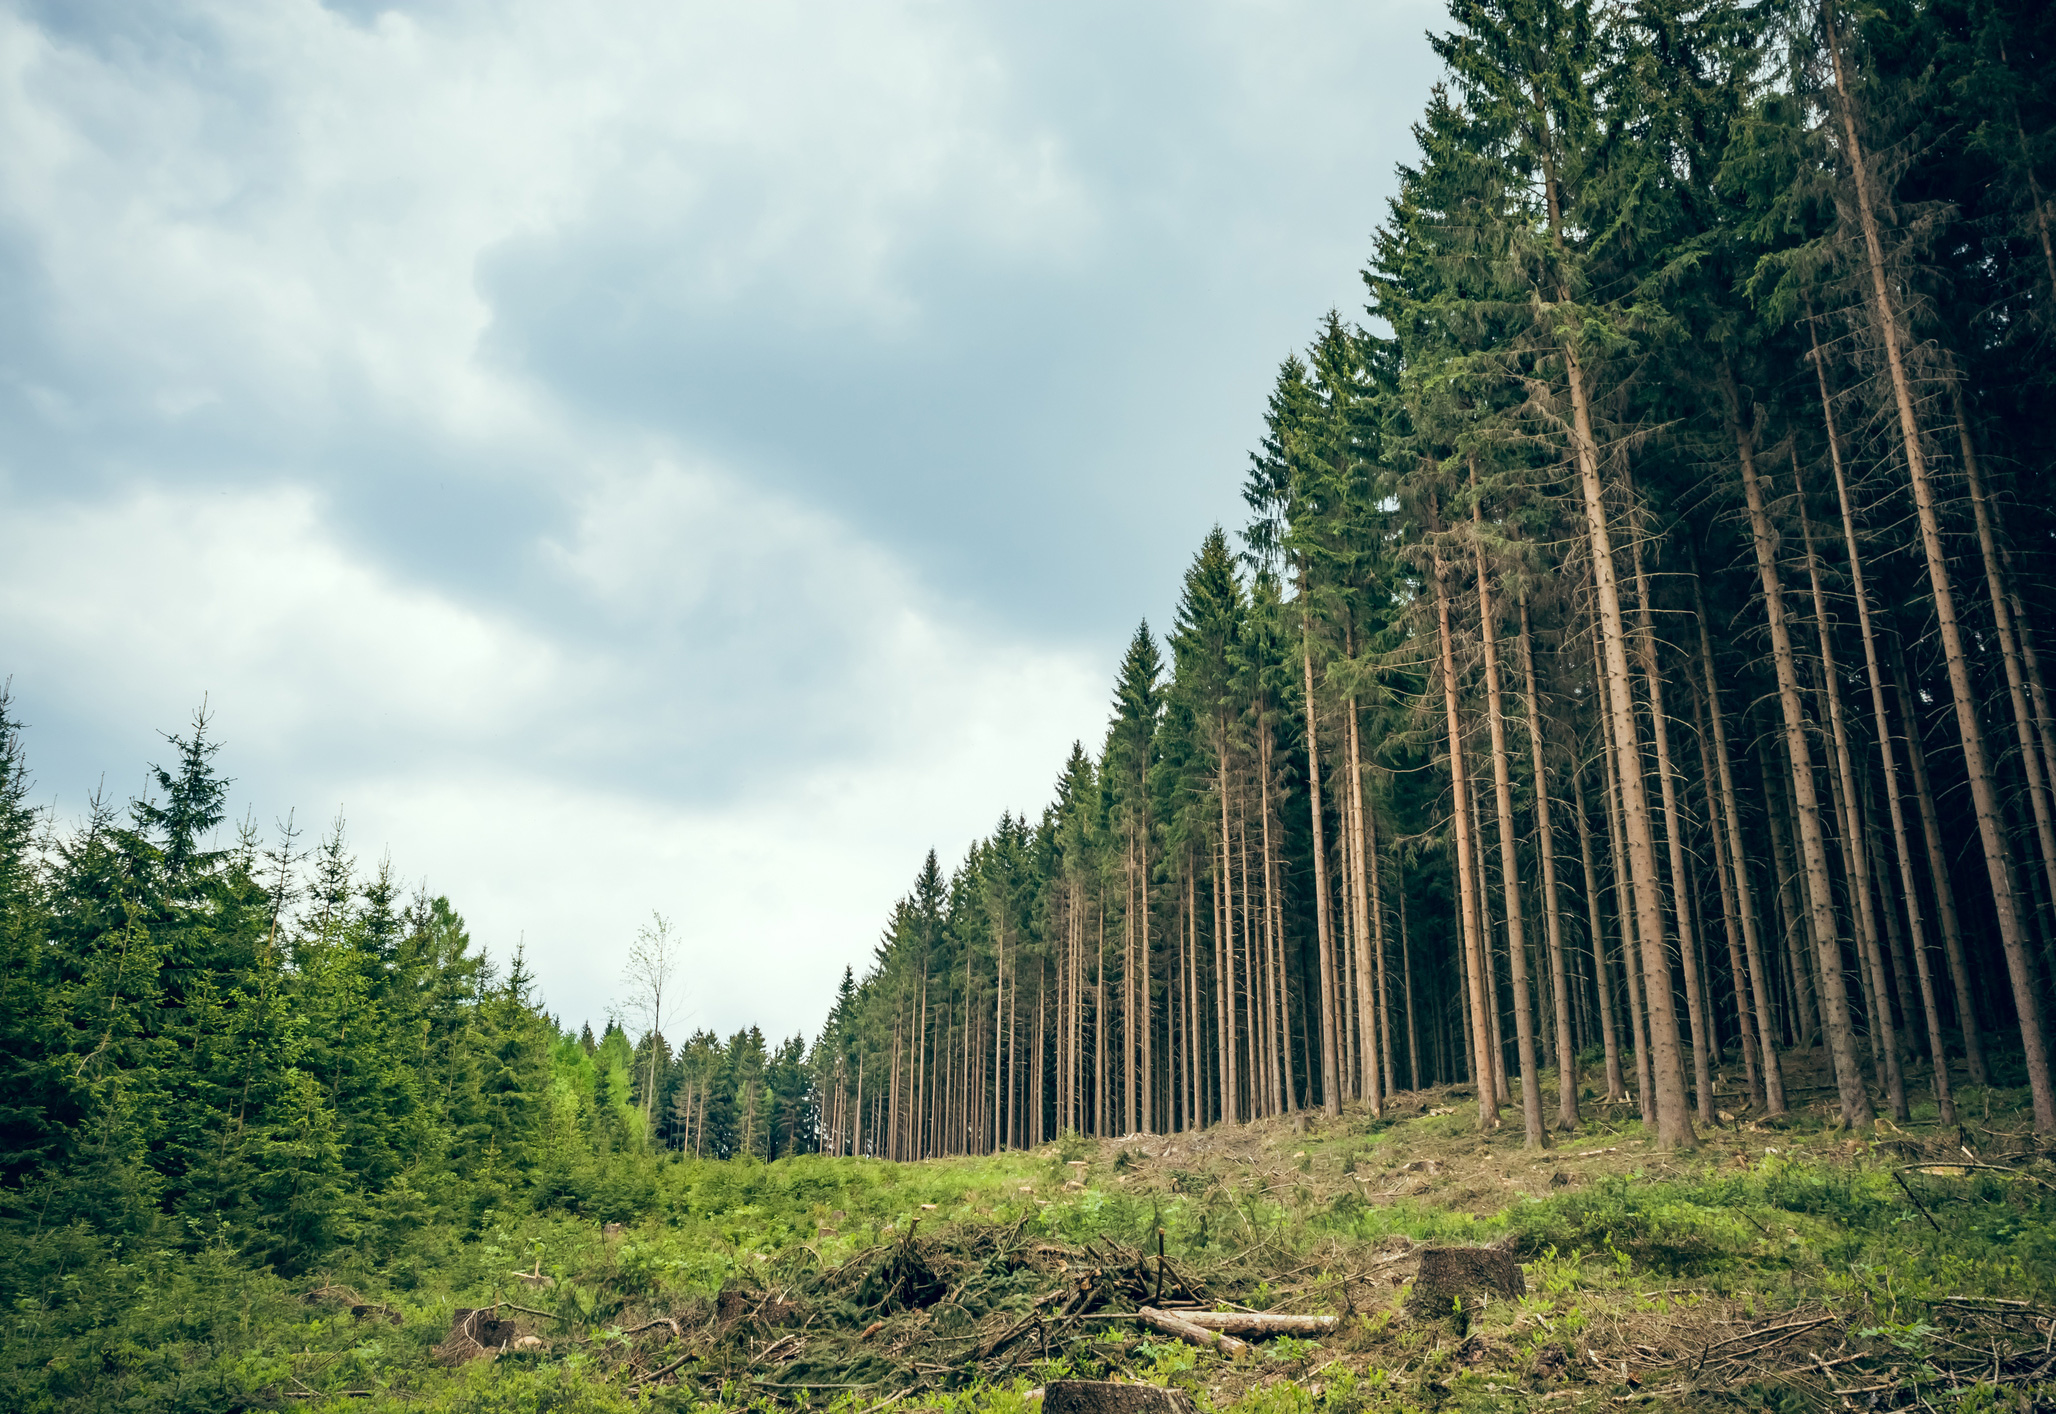
\includegraphics[keepaspectratio,
                                 width=\paperwidth]{images/forest-cut.jpg}
            };
        \end{tikzpicture}
     \end{frame}
}

{ % all template changes are local to this group.
%%    \setbeamertemplate{navigation symbols}{}
    \begin{frame}<article:0>[plain]
      \frametitle{}
        \begin{tikzpicture}[remember picture,overlay]
            \node[at=(current page.center)] {
                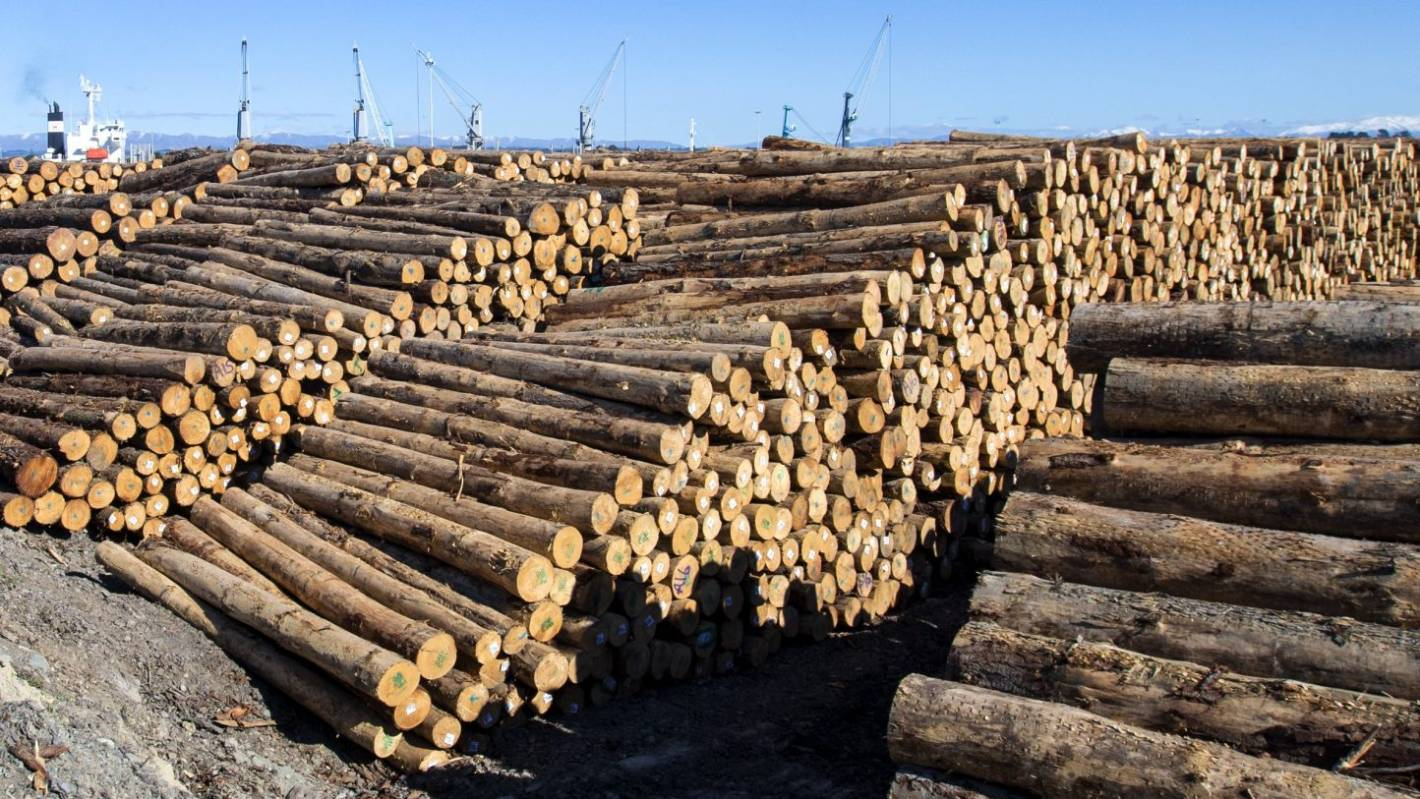
\includegraphics[keepaspectratio,
                                 width=\paperwidth]{images/sawn-logs.jpg}
            };
        \end{tikzpicture}
     \end{frame}
}






{ % all template changes are local to this group.
%%    \setbeamertemplate{navigation symbols}{}
    \begin{frame}<article:0>[plain]
      \frametitle{}
        \begin{tikzpicture}[remember picture,overlay]
            \node[at=(current page.center)] {
                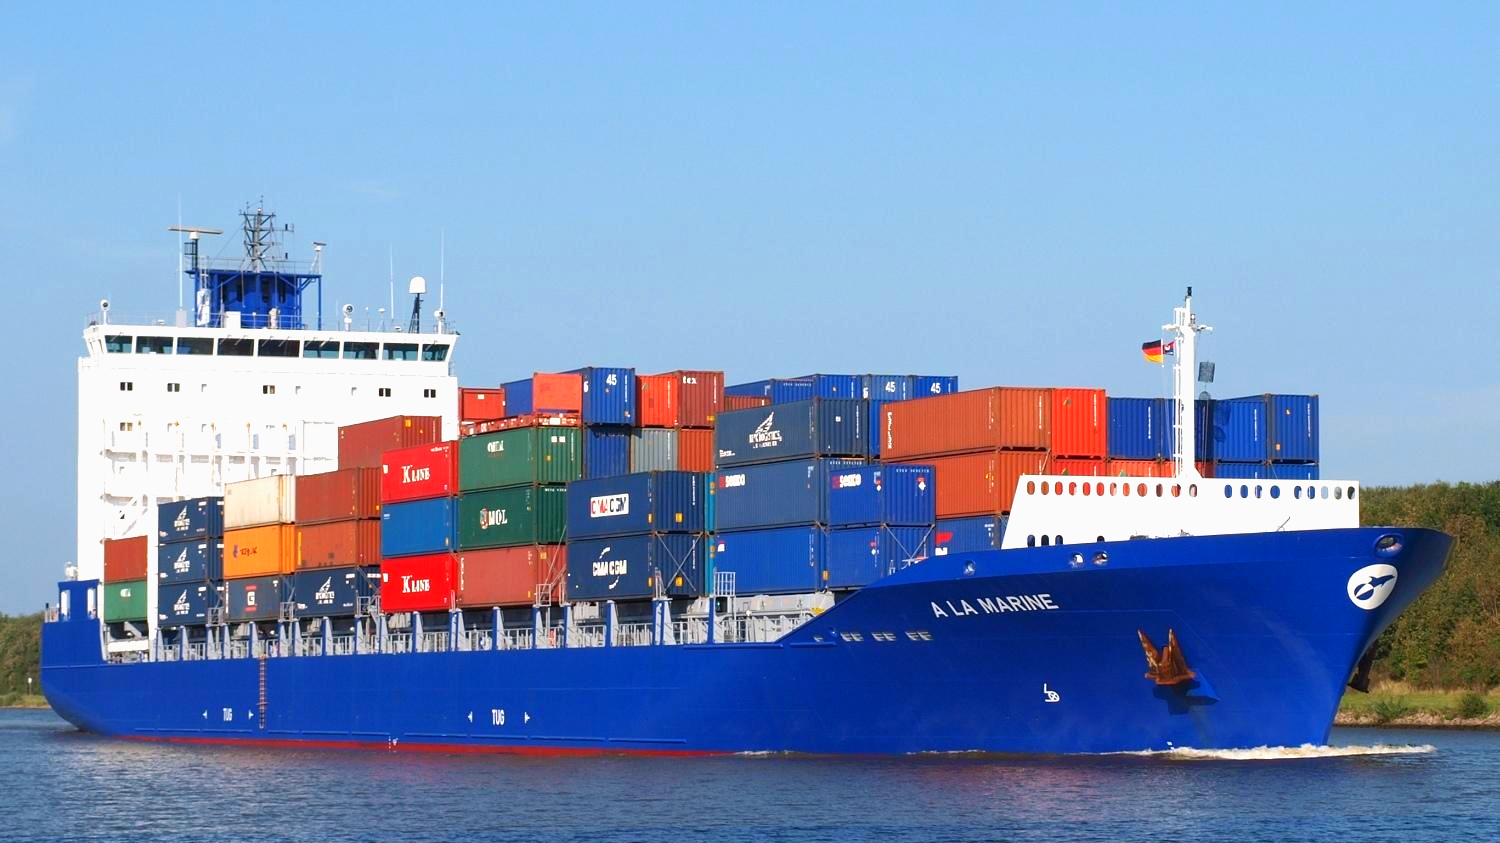
\includegraphics[keepaspectratio,
                                 width=\paperwidth]{images/shipping-ship.jpg}
            };
        \end{tikzpicture}
     \end{frame}
}


{ % all template changes are local to this group.
%%    \setbeamertemplate{navigation symbols}{}
    \begin{frame}<article:0>[plain]
      \frametitle{}
        \begin{tikzpicture}[remember picture,overlay]
            \node[at=(current page.center)] {
                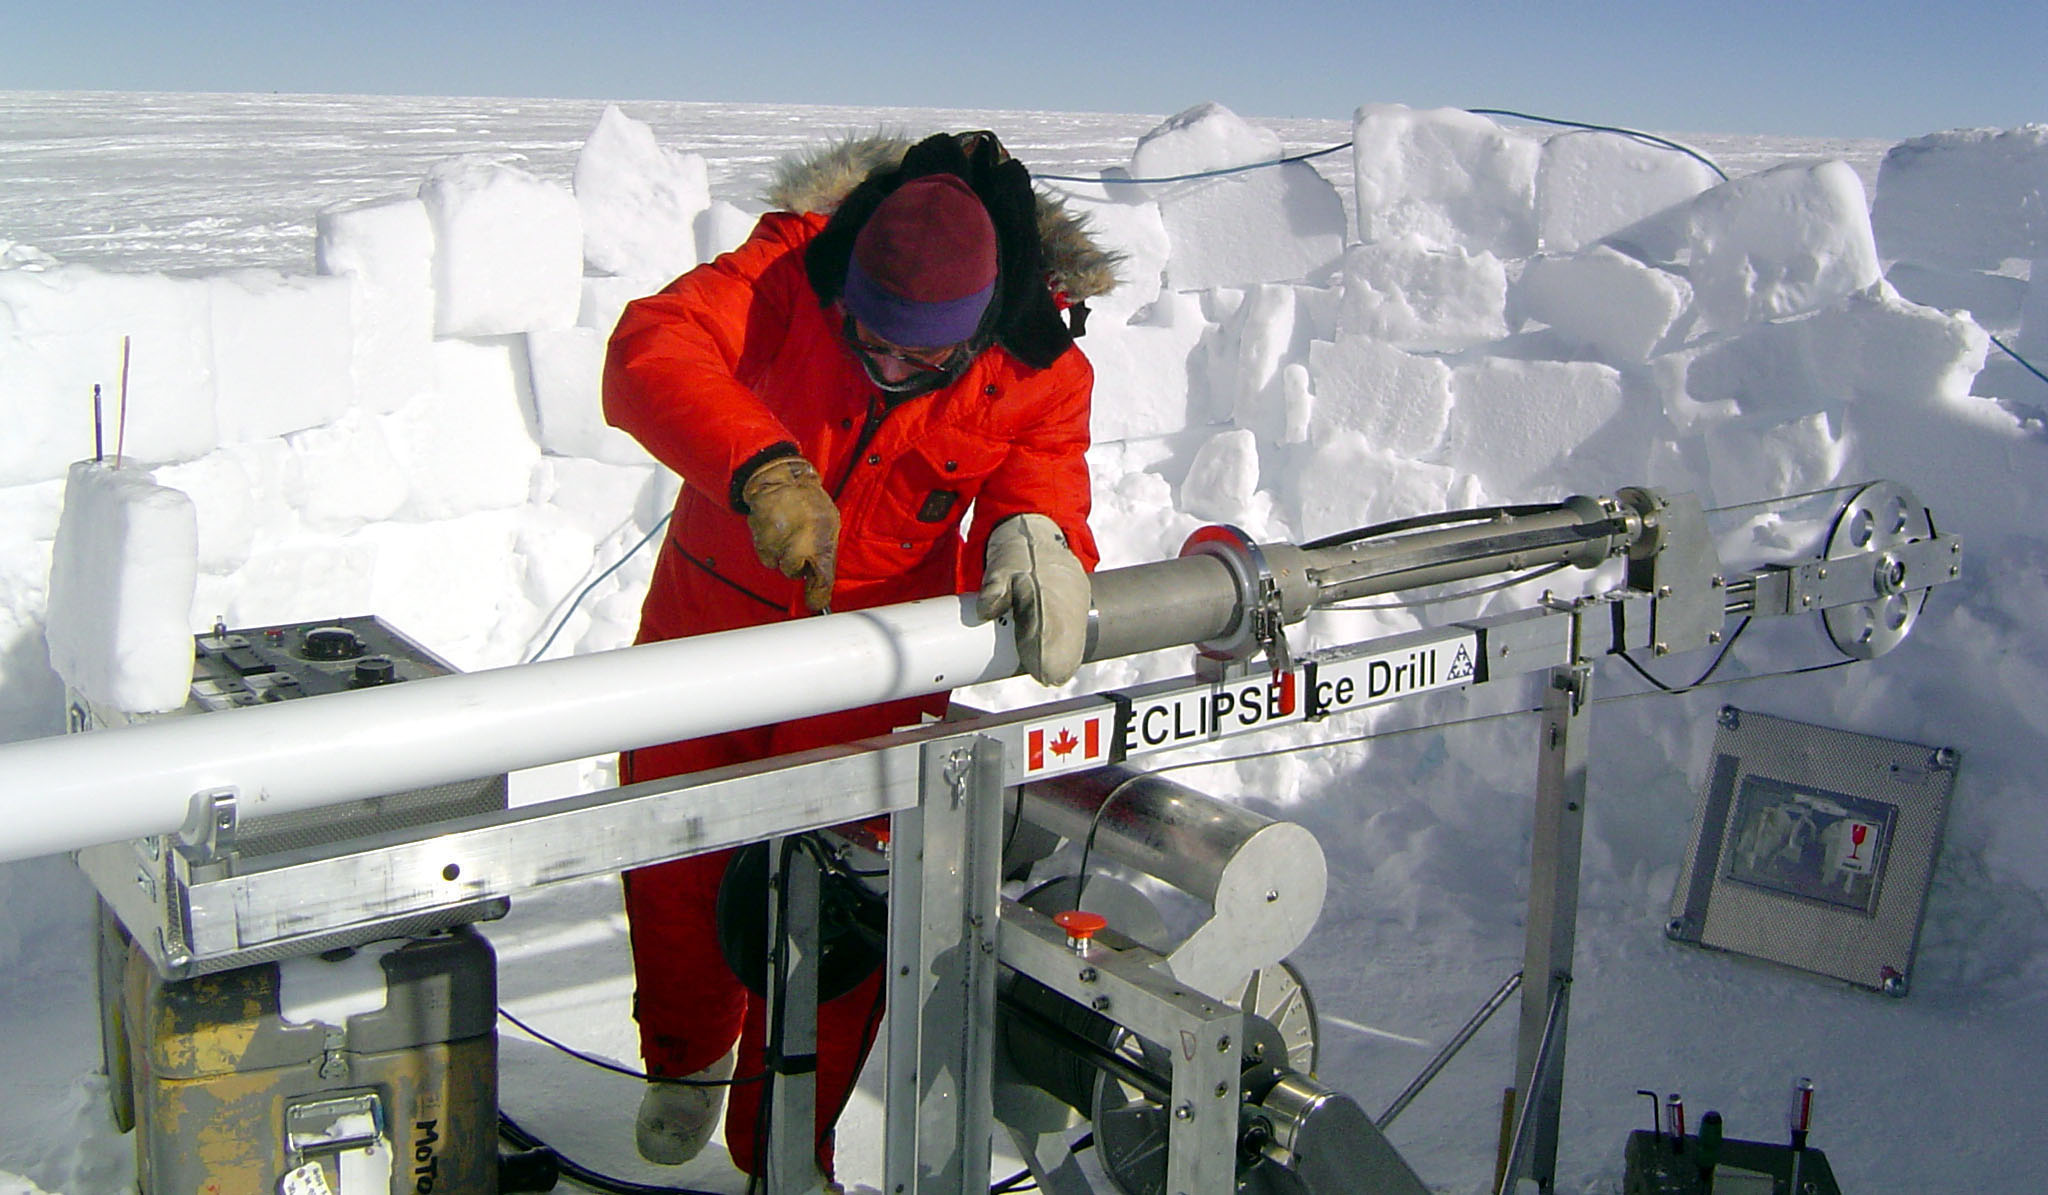
\includegraphics[keepaspectratio,
                                 width=\paperwidth]{images/ice_core.jpg}
            };
        \end{tikzpicture}
  \note[item]{Atmospheric changes = climate change, fire}
     \end{frame}
}

{ % all template changes are local to this group.
%%    \setbeamertemplate{navigation symbols}{}
    \begin{frame}<article:0>[plain]
      \frametitle{}
        \begin{tikzpicture}[remember picture,overlay]
            \node[at=(current page.center)] {
                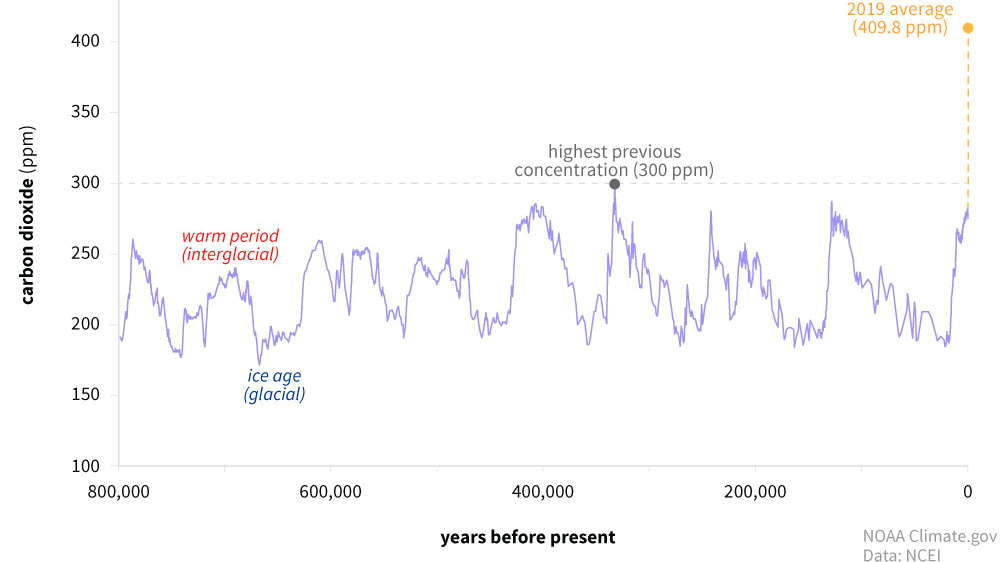
\includegraphics[keepaspectratio,
                                 width=\paperwidth]{images/BAMS_SOTC_2019_co2_paleo_1000px.jpg}
            };
        \end{tikzpicture}
     \end{frame}
}

{ % all template changes are local to this group.
%%    \setbeamertemplate{navigation symbols}{}
    \begin{frame}<article:0>[plain]
      \frametitle{}
        \begin{tikzpicture}[remember picture,overlay]
            \node[at=(current page.center)] {
                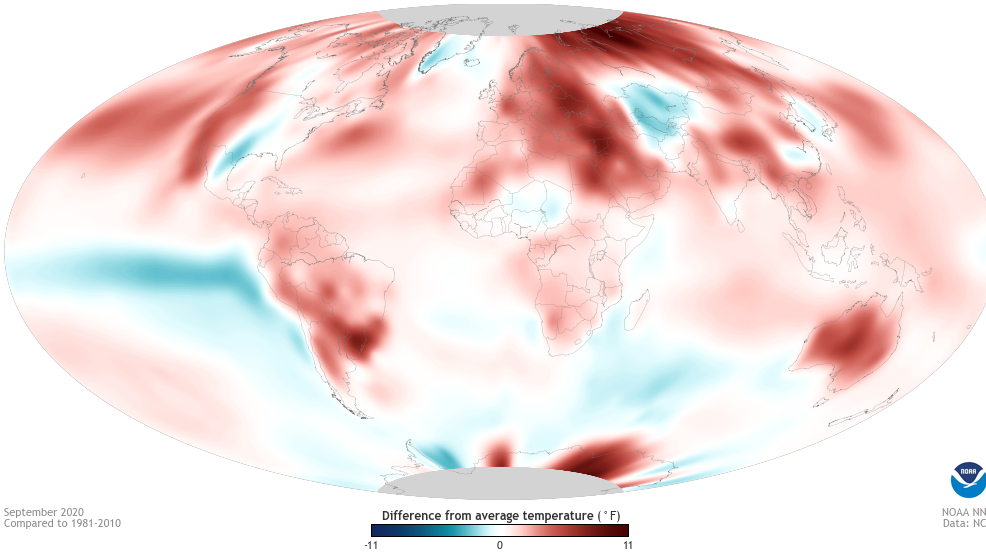
\includegraphics[keepaspectratio,
                                 width=\paperwidth]{images/September_CC2020.png}
            };
        \end{tikzpicture}
     \end{frame}
}

{ % all template changes are local to this group.
%%    \setbeamertemplate{navigation symbols}{}
    \begin{frame}<article:0>[plain]
      \frametitle{}
        \begin{tikzpicture}[remember picture,overlay]
            \node[at=(current page.center)] {
                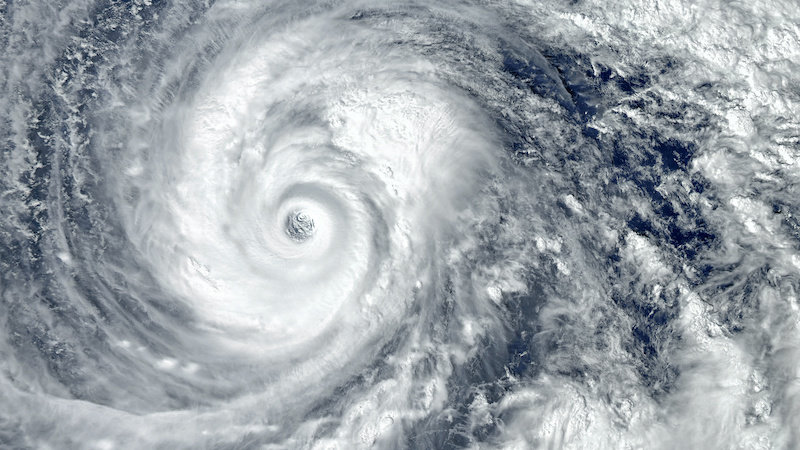
\includegraphics[keepaspectratio,
                                 width=\paperwidth]{images/hurricane.jpg}
            };
        \end{tikzpicture}
     \note[item]{Climate change is causing hurricanes that make
     landfall to take more time to weaken, reports a study published
     11th November 2020 in the journal Nature.}
     \end{frame}
}

{ % all template changes are local to this group.
%%    \setbeamertemplate{navigation symbols}{}
    \begin{frame}<article:0>[plain]
      \frametitle{}
        \begin{tikzpicture}[remember picture,overlay]
            \node[at=(current page.center)] {
                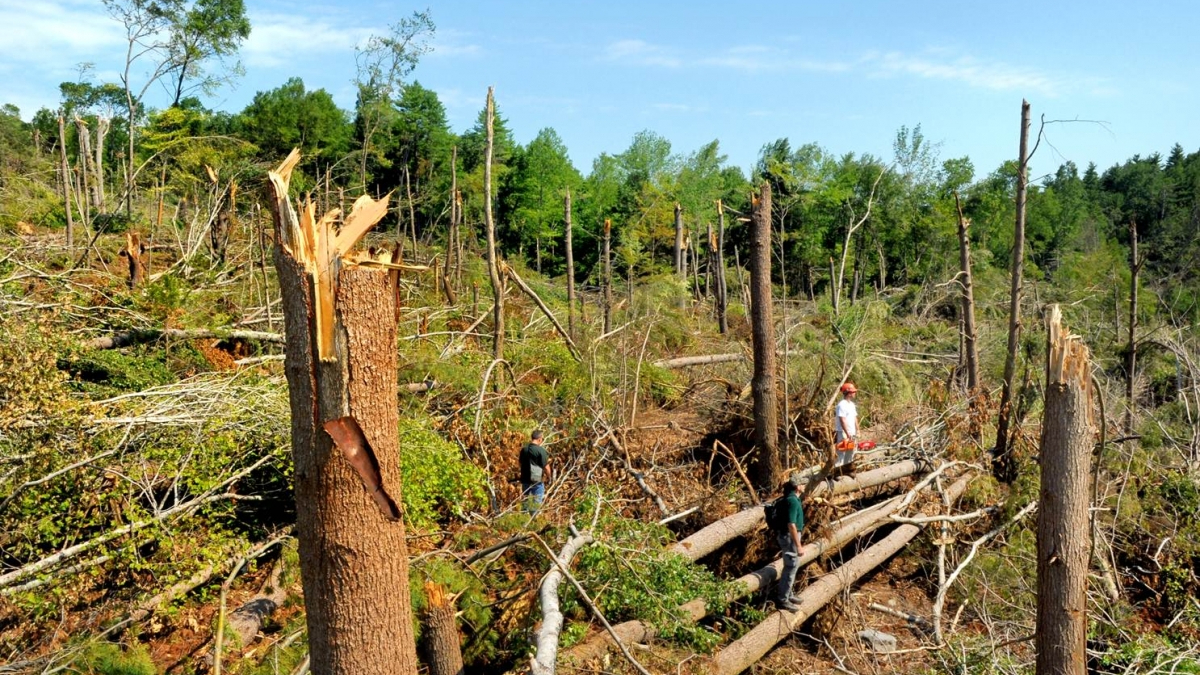
\includegraphics[keepaspectratio,
                                 width=\paperwidth]{images/tornado_hf.jpg}
            };
        \end{tikzpicture}
     \note[item]{Tornado damaged Southbridge, MA forest in 2011}
     \end{frame}
}



{ % all template changes are local to this group.
%%    \setbeamertemplate{navigation symbols}{}
    \begin{frame}<article:0>[plain]
      \frametitle{}
        \begin{tikzpicture}[remember picture,overlay]
            \node[at=(current page.center)] {
                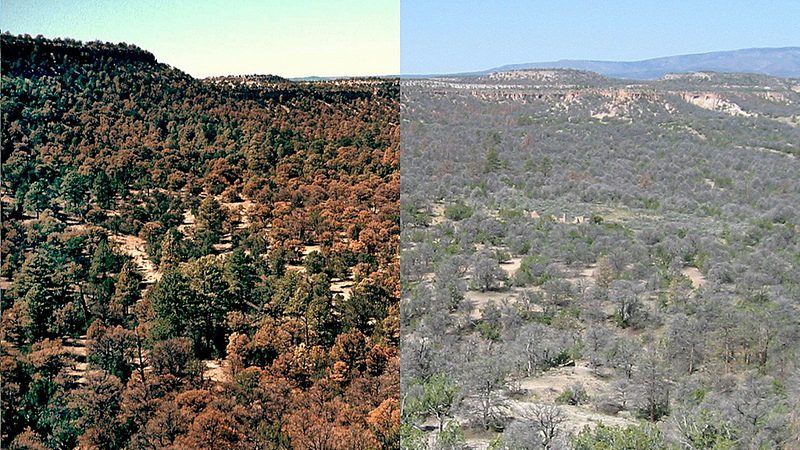
\includegraphics[keepaspectratio,
                                 width=\paperwidth]{images/drought_pjw.jpg}
            };
        \end{tikzpicture}
        \note[item]{Droughts}
     \end{frame}
}



{ % all template changes are local to this group.
%%    \setbeamertemplate{navigation symbols}{}
    \begin{frame}<article:0>[plain]
      \frametitle{}
        \begin{tikzpicture}[remember picture,overlay]
            \node[at=(current page.center)] {
                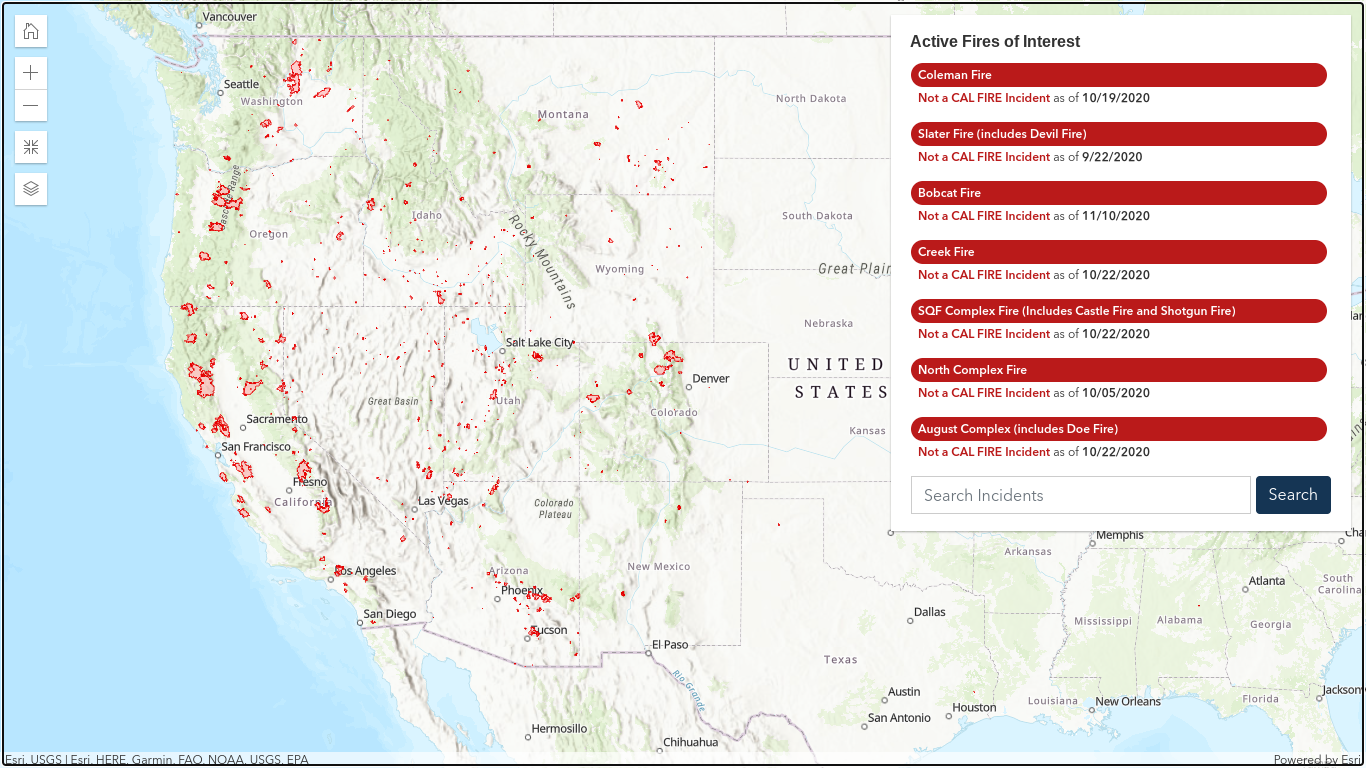
\includegraphics[keepaspectratio,
                                  width=\paperwidth]{images/fires_CALFIRE.png}
            };
        \end{tikzpicture}
        \note[item]{CAL FIRE MAP Tue 17 Nov 2020 12:10:52 PM EST}
     \end{frame}
}


{ % all template changes are local to this group.
%%    \setbeamertemplate{navigation symbols}{}
    \begin{frame}<article:0>[plain]
      \frametitle{}
        \begin{tikzpicture}[remember picture,overlay]
            \node[at=(current page.center)] {
                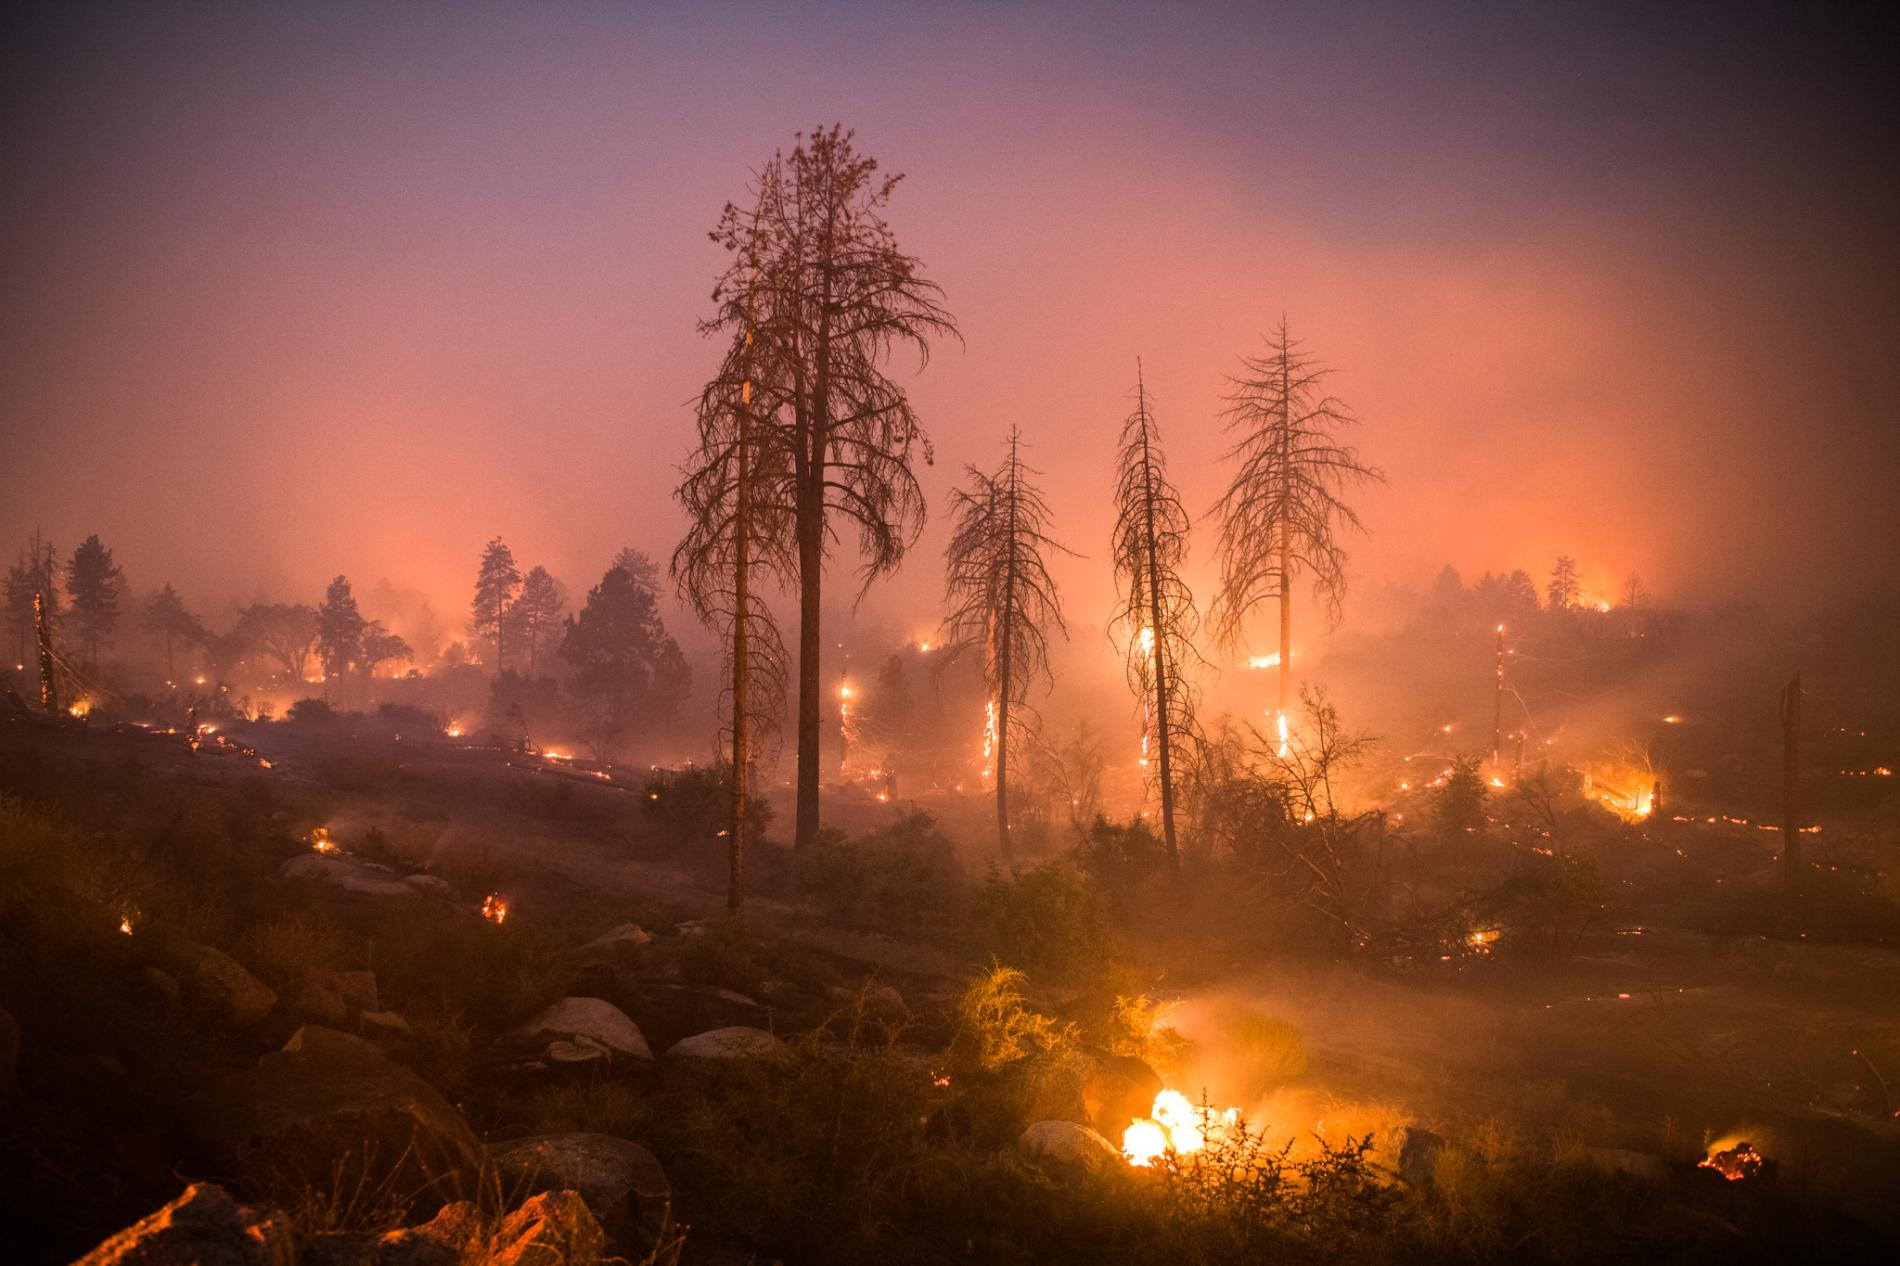
\includegraphics[keepaspectratio,
                                 width=\paperwidth]{images/fires_CAcranston.jpg}
            };
        \end{tikzpicture}
        \note[item]{CA Cranston Riverside 2018}
     \end{frame}
}


{ % all template changes are local to this group.
%%    \setbeamertemplate{navigation symbols}{}
    \begin{frame}<article:0>[plain]
      \frametitle{}
        \begin{tikzpicture}[remember picture,overlay]
            \node[at=(current page.center)] {
                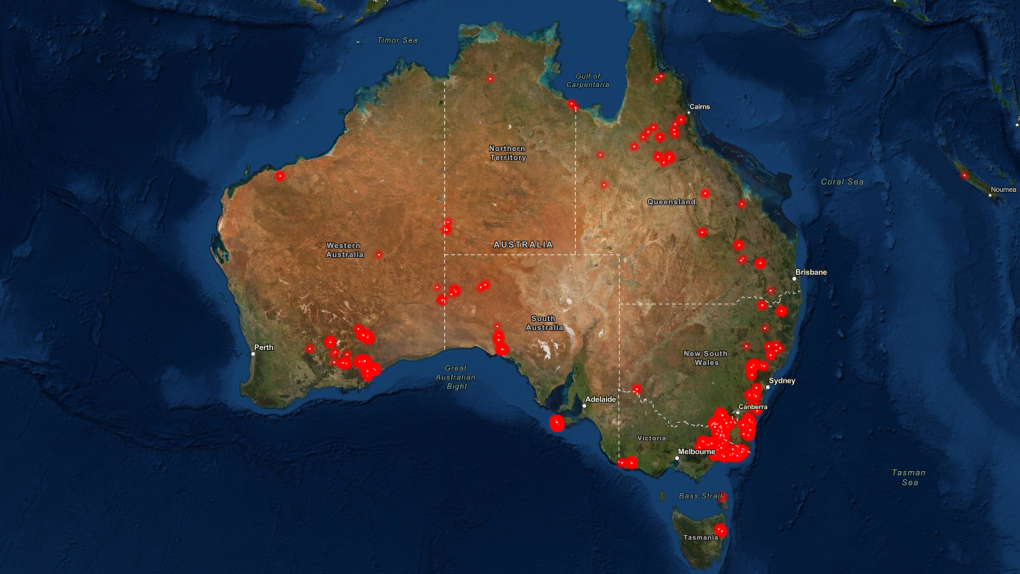
\includegraphics[keepaspectratio,
                                 width=\paperwidth]{images/fires_AUS.png}
            };
        \end{tikzpicture}
        \note[item]{Fires in Australia 2020}
     \end{frame}
}







\begin{frame}
  \frametitle{Forests in the Anthropocence}
  
  \begin{itemize}
  \item Forests are changing from human impacts \pause
  \item Large direct and \underline{indirect} effects of land-use  \pause
  \item How do we address indirect and systems-level effects? 
  \end{itemize}

\end{frame}


\begin{frame}
  \frametitle{Today's Talk}

\tableofcontents

\note[item]{Intro/Context}
\note[item]{Global forest loss and gain and change}
\note[item]{Global greening = India(Agriculture) + China(Forests)}
\note[item]{Economics*Ecology = Landscape Extended Models}
\note[item]{Network Analysis of China's Greening}
\note[item]{Global Scale}
\note[item]{Local Scale}
\note[item]{Landscape = Tian 2019, Chen 2019}
\note[item]{Resilience Analysis of China's Forest LE-MRIO}
\note[item]{Conclusions and Future Work}
\note[item]{Acknowledgements}

\end{frame}



\section{Environmental Extended Economic Models}


\begin{frame}
  \frametitle{Input-Output Models}
\end{frame}



{ 
\begin{frame}<article:0>[plain]
   \frametitle{}
      \begin{tikzpicture}[remember picture,overlay]
         \node[at=(current page.center)] {
             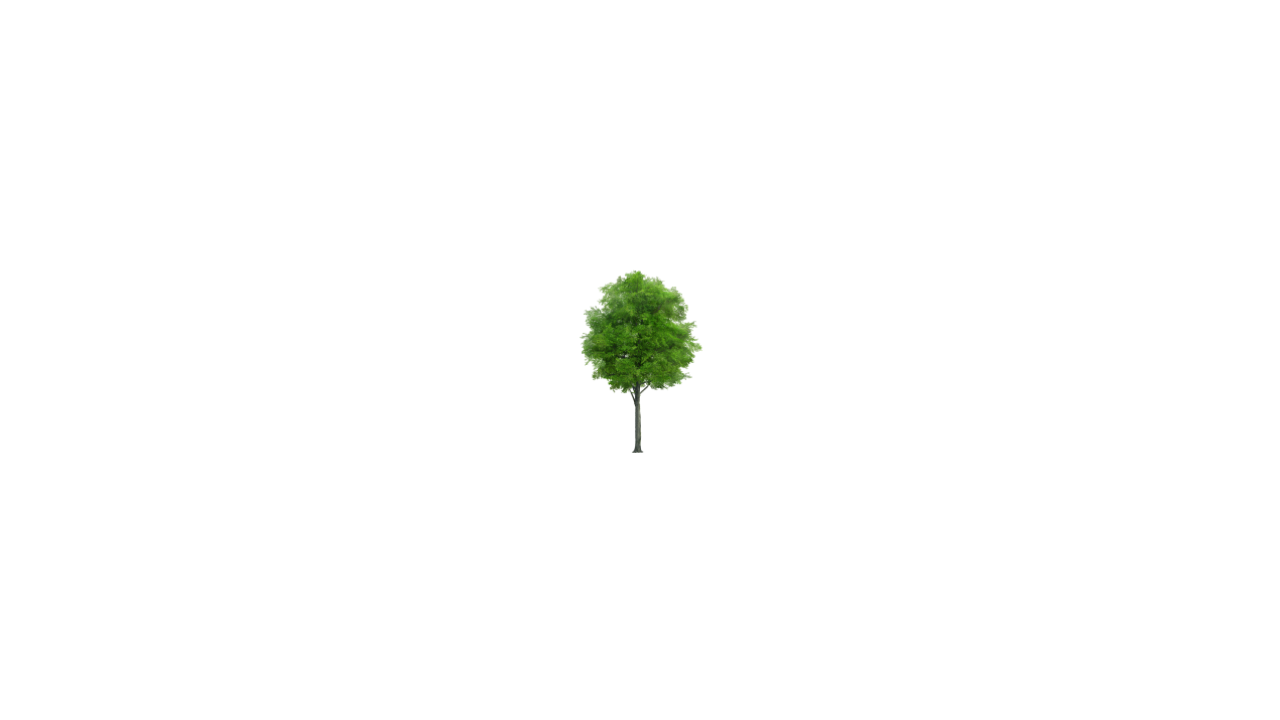
\includegraphics[keepaspectratio,
                              width=\paperwidth]{images/le-mrio.png}
            };
      \end{tikzpicture}
     \note[]{}
\end{frame}
}

{ 
\begin{frame}<article:0>[plain]
   \frametitle{}
      \begin{tikzpicture}[remember picture,overlay]
         \node[at=(current page.center)] {
             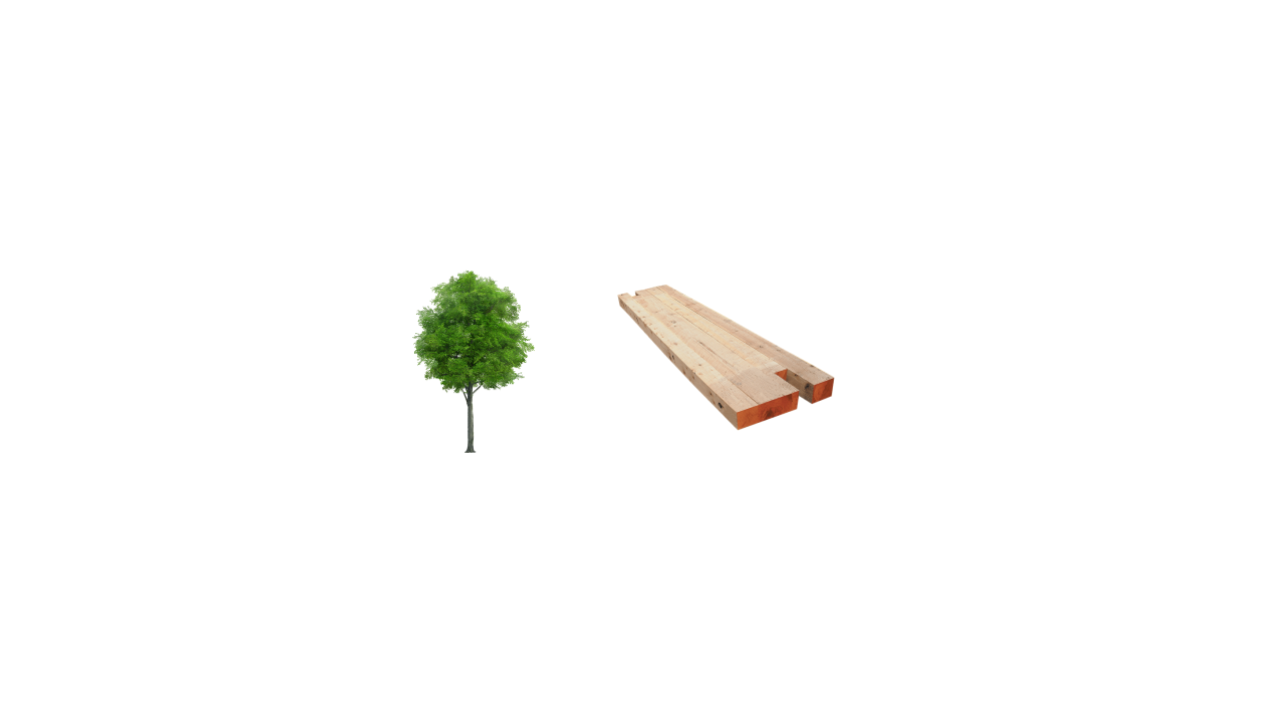
\includegraphics[keepaspectratio,
                              width=\paperwidth]{images/le-mrio-1.png}
            };
      \end{tikzpicture}
     \note[]{}
\end{frame}
}

{ 
\begin{frame}<article:0>[plain]
   \frametitle{}
      \begin{tikzpicture}[remember picture,overlay]
         \node[at=(current page.center)] {
             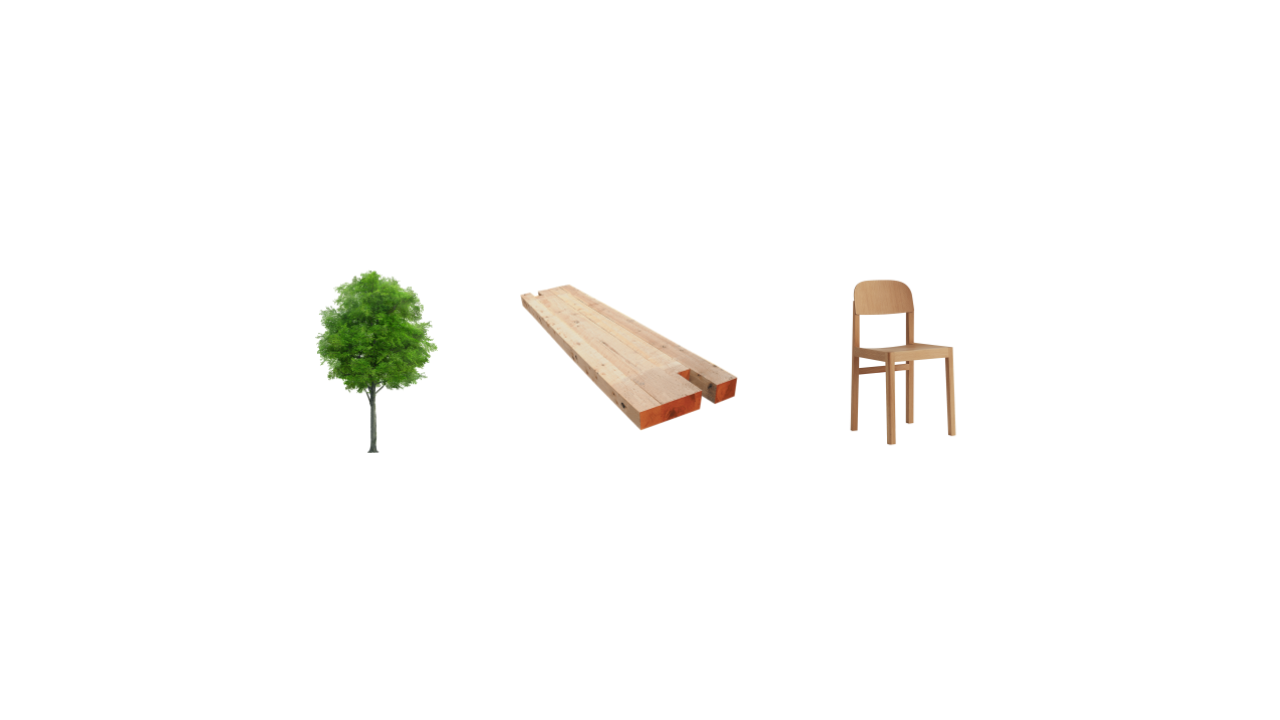
\includegraphics[keepaspectratio,
                              width=\paperwidth]{images/le-mrio-2.png}
            };
      \end{tikzpicture}
     \note[]{}
\end{frame}
}



{ 
\begin{frame}<article:0>[plain]
   \frametitle{}
      \begin{tikzpicture}[remember picture,overlay]
         \node[at=(current page.center)] {
             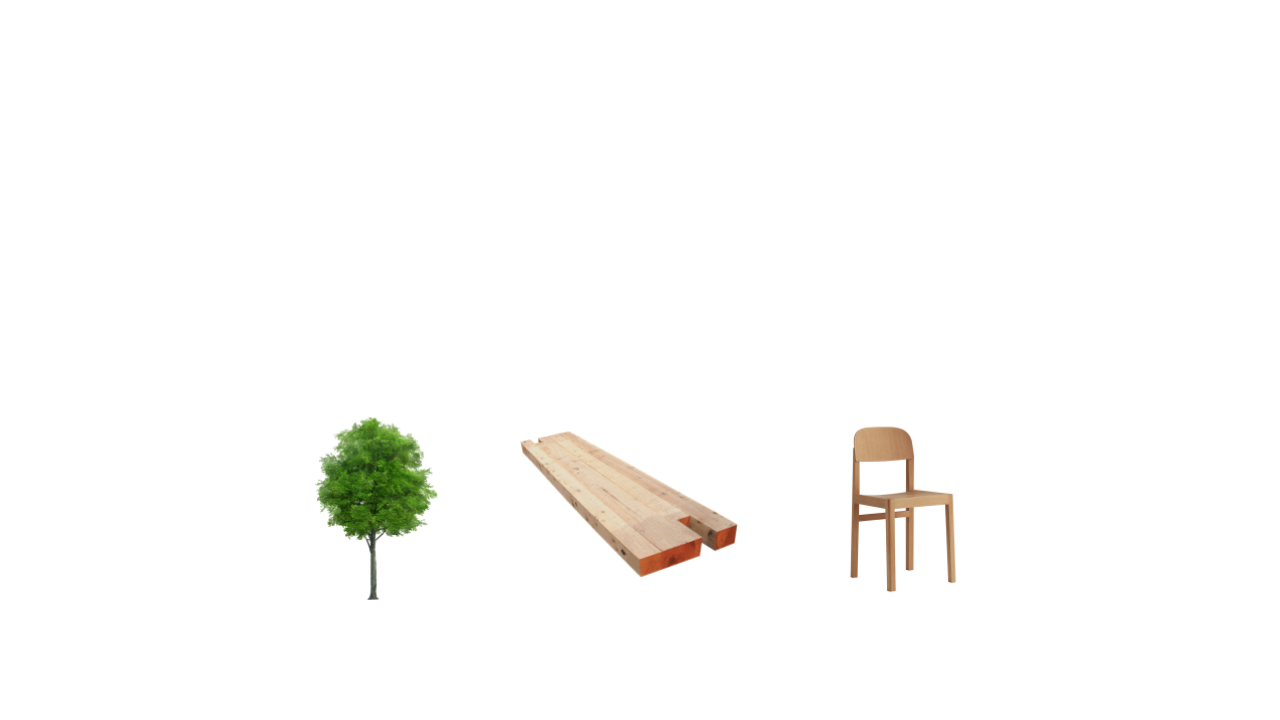
\includegraphics[keepaspectratio,
                              width=\paperwidth]{images/le-mrio-3.png}
            };
      \end{tikzpicture}
     \note[]{}
\end{frame}
}



{ 
\begin{frame}<article:0>[plain]
   \frametitle{}
      \begin{tikzpicture}[remember picture,overlay]
         \node[at=(current page.center)] {
             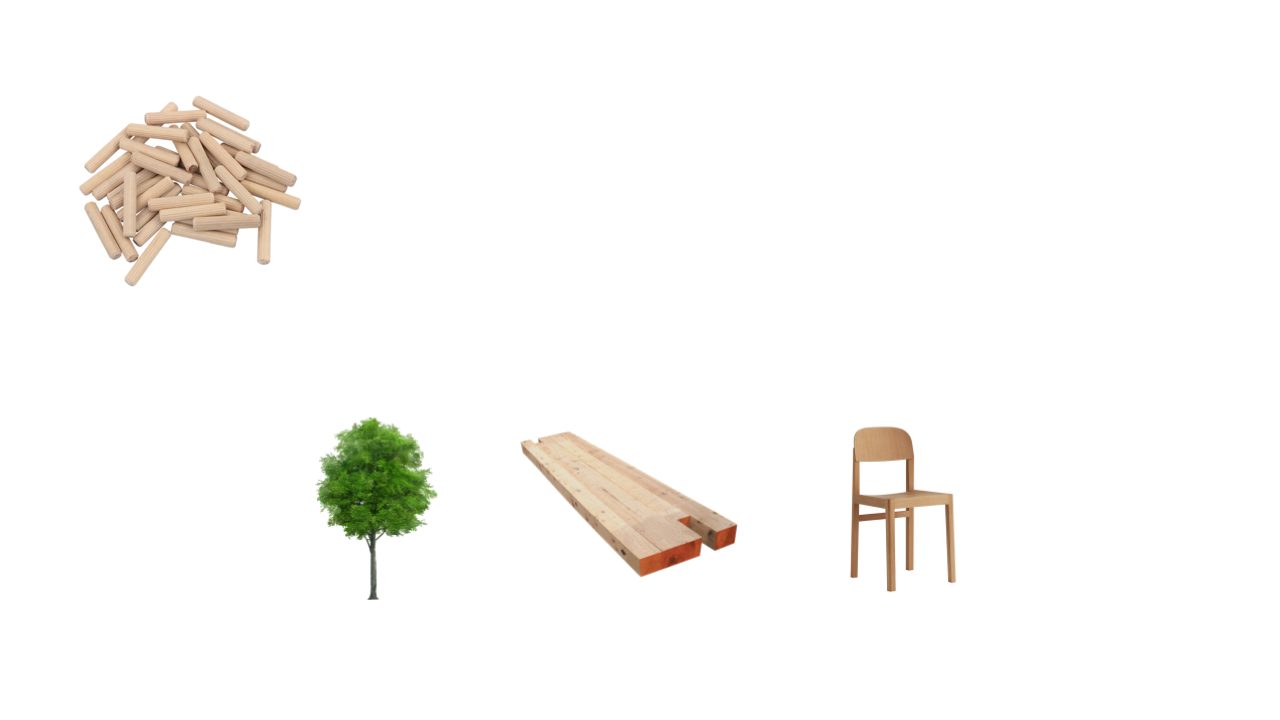
\includegraphics[keepaspectratio,
                              width=\paperwidth]{images/le-mrio-4.png}
            };
      \end{tikzpicture}
     \note[]{}
\end{frame}
}



{ 
\begin{frame}<article:0>[plain]
   \frametitle{}
      \begin{tikzpicture}[remember picture,overlay]
         \node[at=(current page.center)] {
             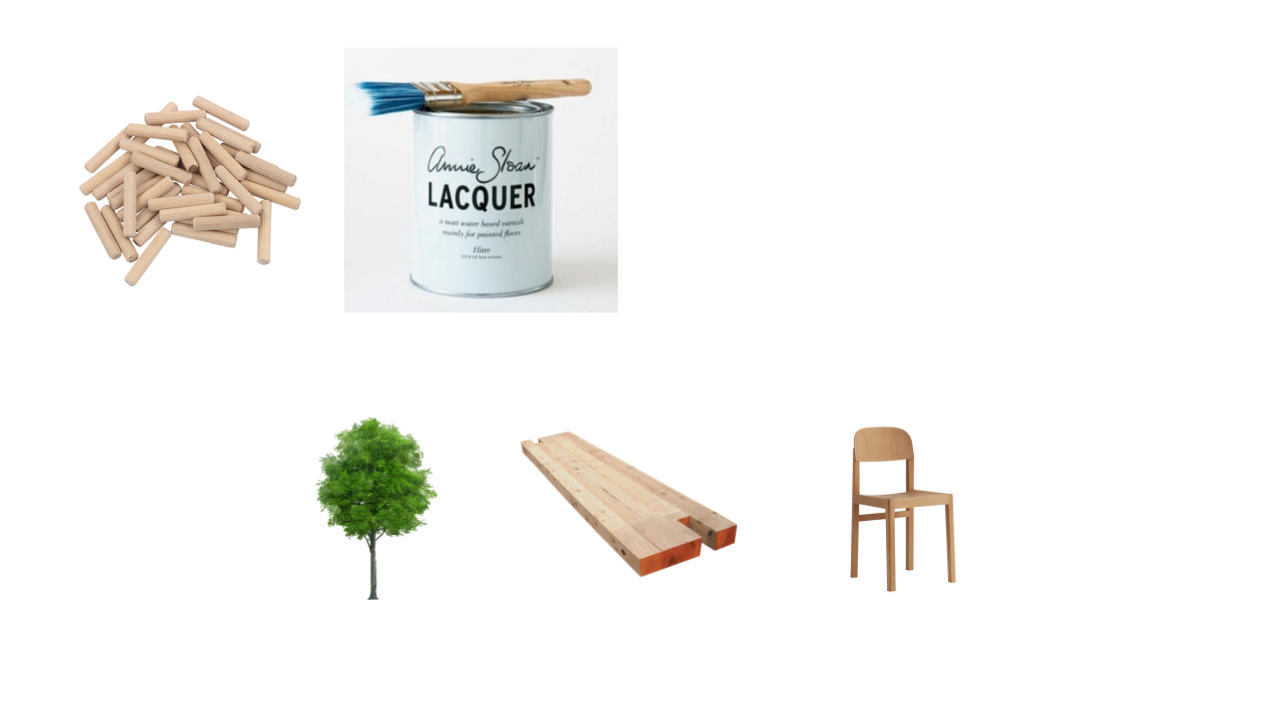
\includegraphics[keepaspectratio,
                              width=\paperwidth]{images/le-mrio-5.png}
            };
      \end{tikzpicture}
     \note[]{}
\end{frame}
}



{ 
\begin{frame}<article:0>[plain]
   \frametitle{}
      \begin{tikzpicture}[remember picture,overlay]
         \node[at=(current page.center)] {
             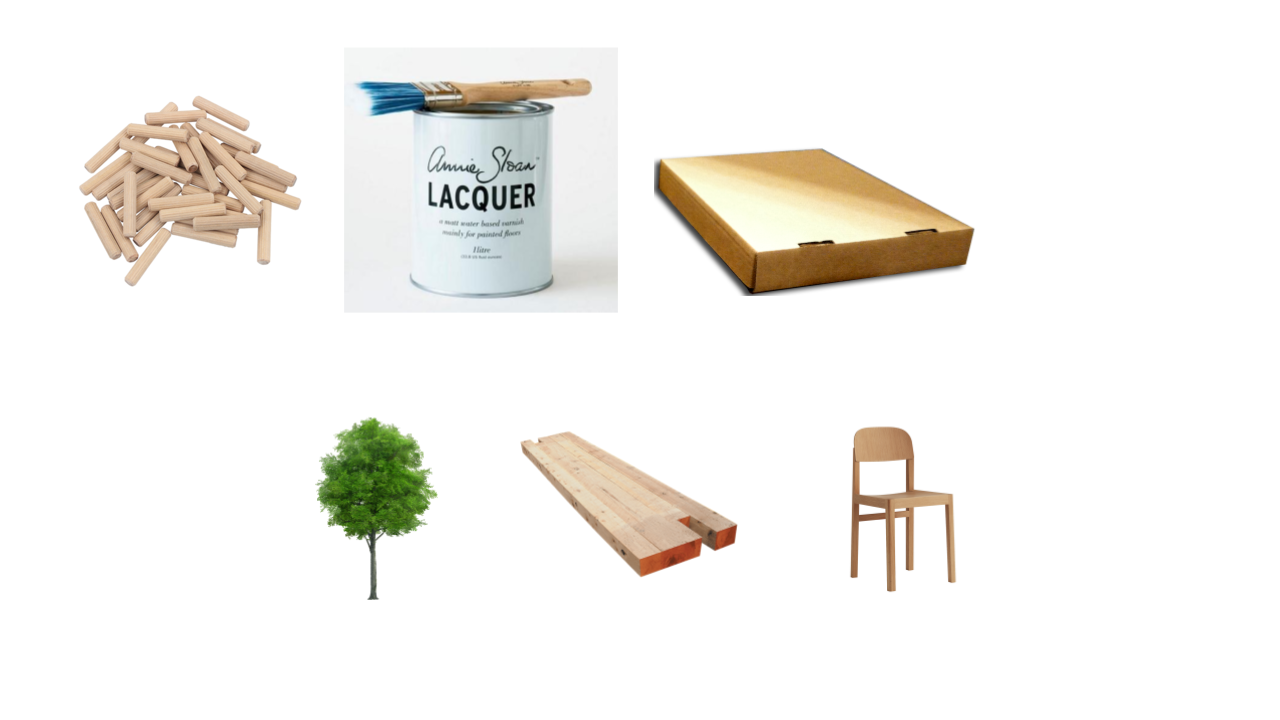
\includegraphics[keepaspectratio,
                              width=\paperwidth]{images/le-mrio-6.png}
            };
      \end{tikzpicture}
     \note[]{}
\end{frame}
}



{ 
\begin{frame}<article:0>[plain]
   \frametitle{}
      \begin{tikzpicture}[remember picture,overlay]
         \node[at=(current page.center)] {
             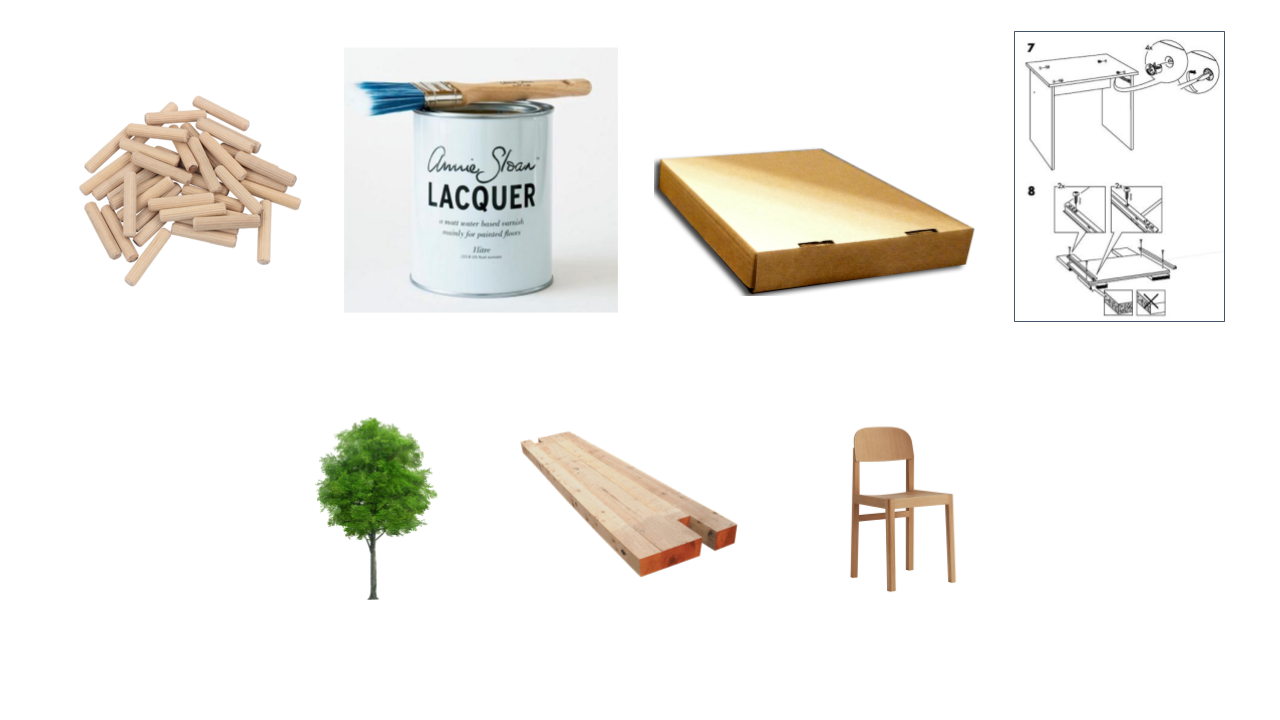
\includegraphics[keepaspectratio,
                              width=\paperwidth]{images/le-mrio-7.png}
            };
      \end{tikzpicture}
     \note[]{}
\end{frame}
}

{ 
\begin{frame}<article:0>[plain]
   \frametitle{}
      \begin{tikzpicture}[remember picture,overlay]
         \node[at=(current page.center)] {
             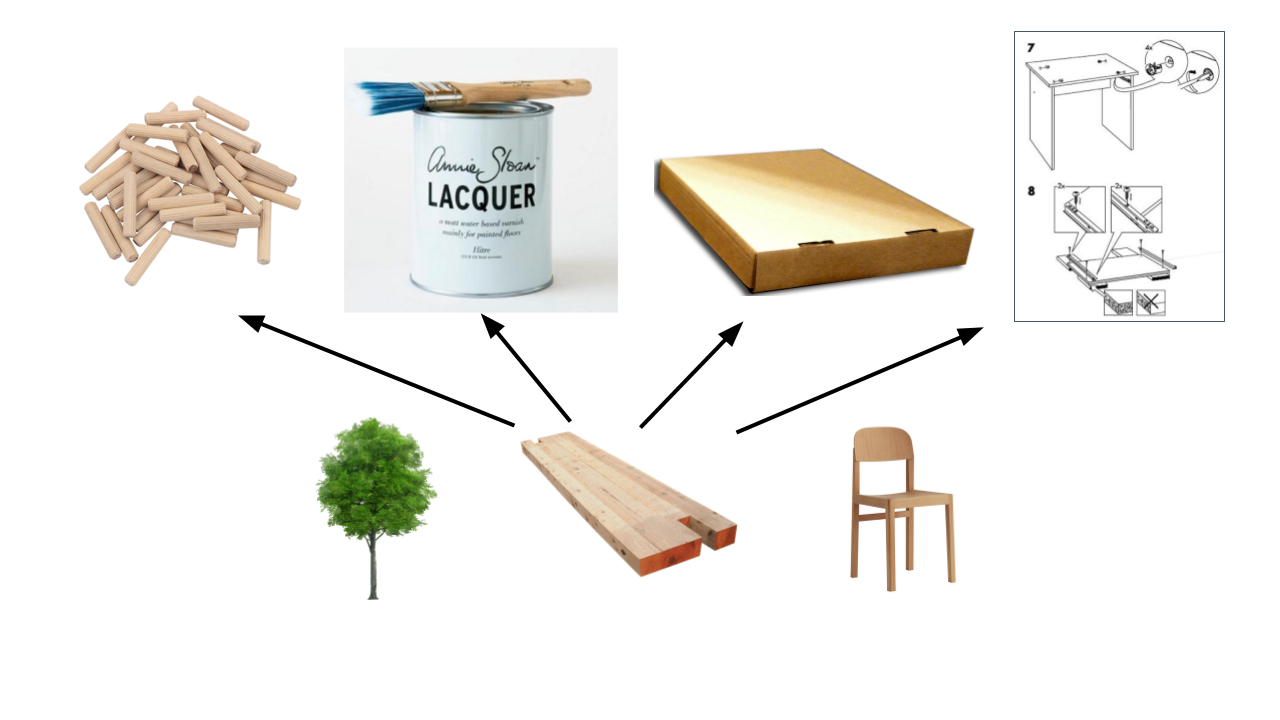
\includegraphics[keepaspectratio,
                              width=\paperwidth]{images/le-mrio-8.png}
            };
      \end{tikzpicture}
     \note[]{}
\end{frame}
}

{ 
\begin{frame}<article:0>[plain]
   \frametitle{}
      \begin{tikzpicture}[remember picture,overlay]
         \node[at=(current page.center)] {
             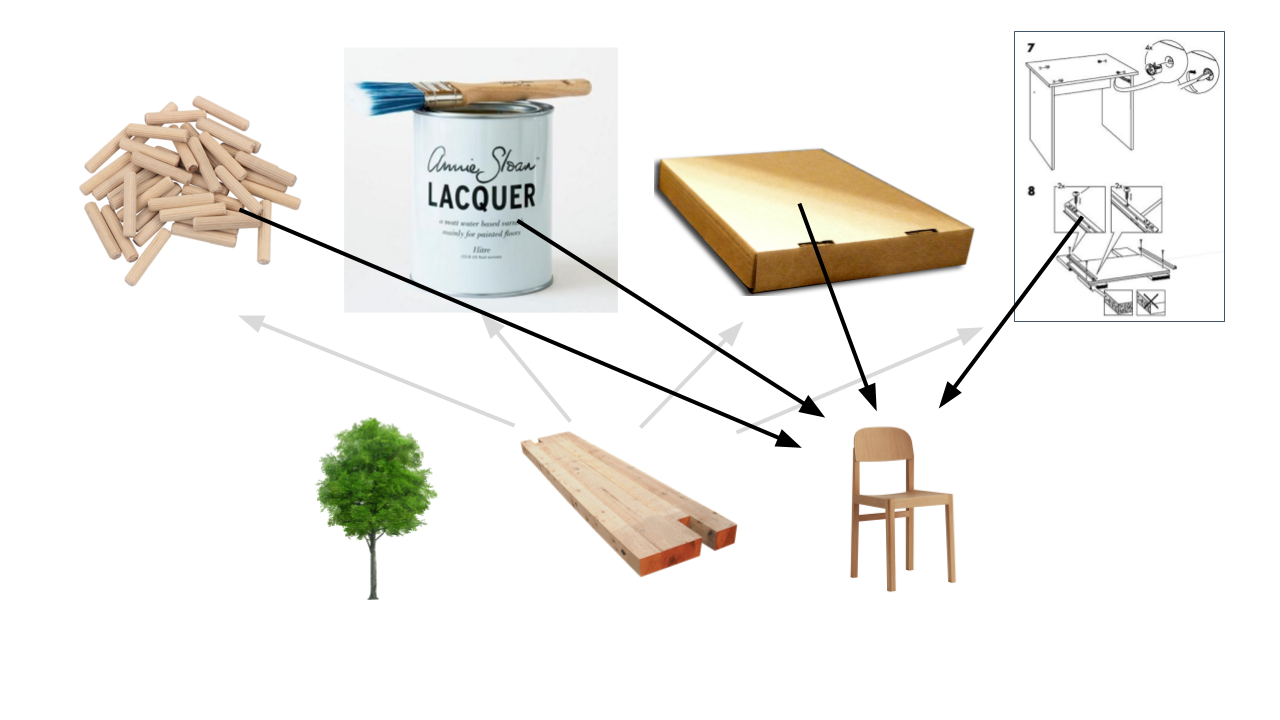
\includegraphics[keepaspectratio,
                              width=\paperwidth]{images/le-mrio-9.png}
            };
      \end{tikzpicture}
     \note[]{}
\end{frame}
}

\begin{frame}
  \frametitle{Input-Output Modeling}
\begin{columns}
\begin{column}{0.5\textwidth}
\begin{center}
$X = (I - A)^{-1}Y$
\end{center}
\end{column}
\begin{column}{0.5\textwidth}  %%<--- here
\end{column}
\end{columns}
\end{frame}

\begin{frame}
  \frametitle{Input-Output Modeling}
\begin{columns}
\begin{column}{0.5\textwidth}
\begin{center}
$X = (I - A)^{-1}Y$
\end{center}
\end{column}
\begin{column}{0.5\textwidth}  %%<--- here
  \begin{itemize}
  \item Uses a simple subtraction to calculate all of the indirect
  consumption correctly \pause
  \item Indirect effects can, and usually are, greater than direct \pause
  \item Has been influencial in ecosystem network analysis
  \end{itemize}
\end{column}
\end{columns}
\end{frame}

\begin{frame}
  \frametitle{Environmental Extended Input-Output Models}
\begin{columns}
\begin{column}{0.5\textwidth}
\begin{center}
$X = (I - A)^{-1}Y$
\end{center}
\end{column}
\begin{column}{0.5\textwidth}  %%<--- here

\end{column}
\end{columns}
\end{frame}

\begin{frame}
  \frametitle{Environmental Extended Input-Output Models}
\begin{columns}
\begin{column}{0.5\textwidth}
\begin{center}
$X = E(I - A)^{-1}Y$
\end{center}
\end{column}
\begin{column}{0.5\textwidth}  %%<--- here

\end{column}
\end{columns}
\end{frame}


\begin{frame}
  \frametitle{Environmental Extended Input-Output Models}
\begin{columns}
\begin{column}{0.5\textwidth}
\begin{center}
$X = E(I - A)^{-1}Y$
\end{center}
\end{column}
\begin{column}{0.5\textwidth}  %%<--- here
  \begin{itemize}
  \item Any environmental (or social) variable can be used \pause
  \item \textbf{Required}: estimate of how much is used by each
  indusrial sector
  \end{itemize}
\end{column}
\end{columns}
\end{frame}

{ 
\begin{frame}<article:0>[plain]
   \frametitle{}
      \begin{tikzpicture}[remember picture,overlay]
         \node[at=(current page.center)] {
             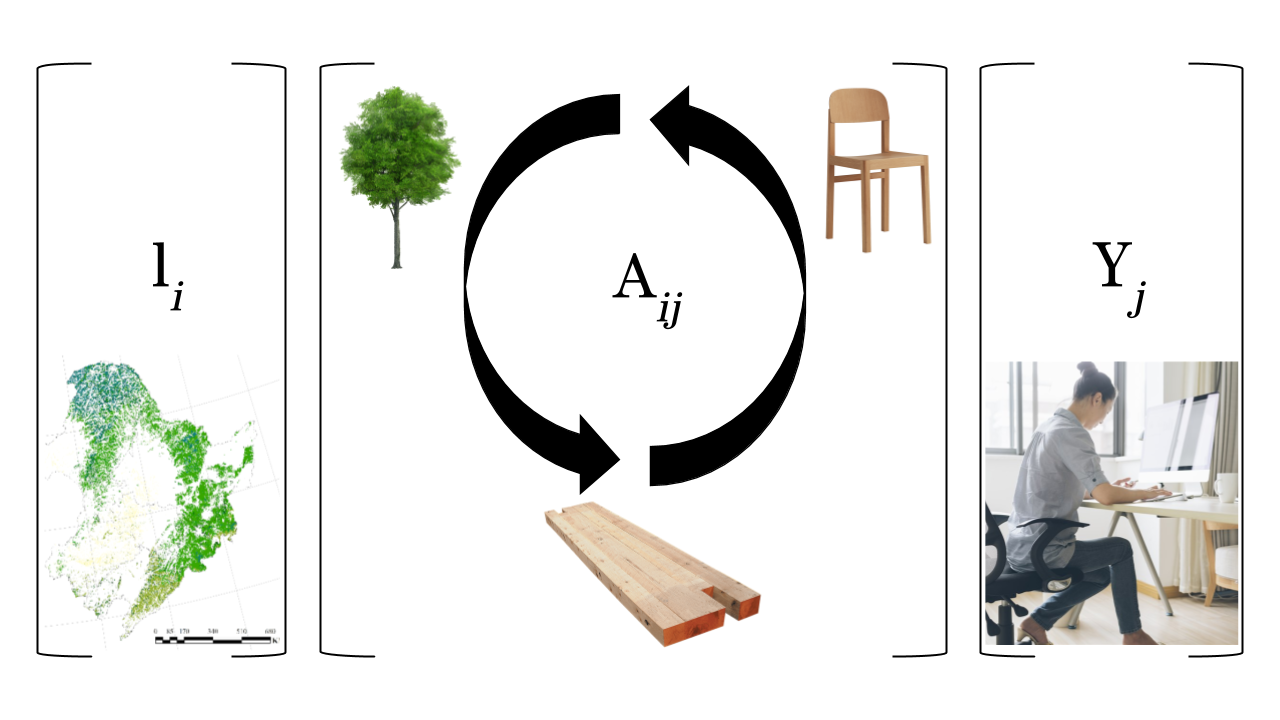
\includegraphics[keepaspectratio,
                              width=\paperwidth]{images/le-mrio-form.png}
            };
      \end{tikzpicture}
     \note[]{}
\end{frame}
}


\begin{frame}
  \frametitle{``Multi-Regional'' = Spatial Context}
\end{frame}


{ %%% blank frame
\begin{frame}<article:0>[plain]
   \frametitle{}
      \begin{tikzpicture}[remember picture,overlay]
         \node[at=(current page.center)] {
             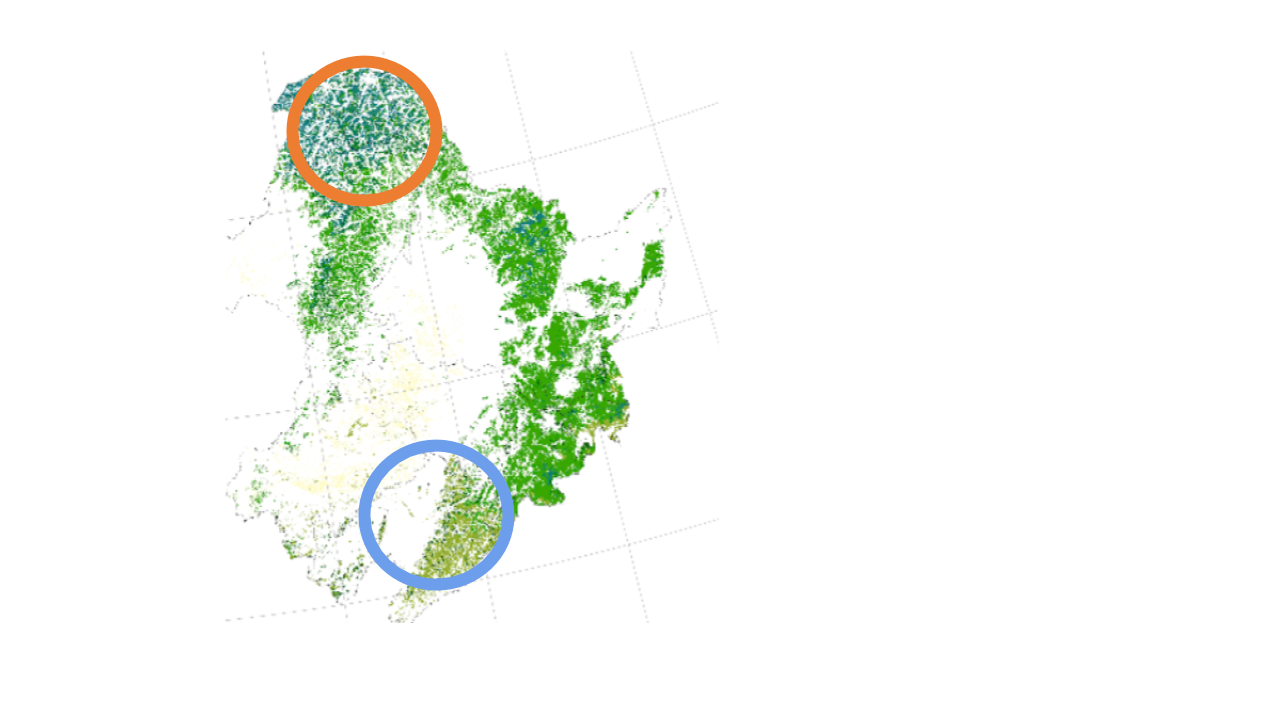
\includegraphics[keepaspectratio,
                              width=\paperwidth]{images/regionalize1.png}
            };
      \end{tikzpicture}
     \note[]{}
\end{frame}
}

{ %%% blank frame
\begin{frame}<article:0>[plain]
   \frametitle{}
      \begin{tikzpicture}[remember picture,overlay]
         \node[at=(current page.center)] {
             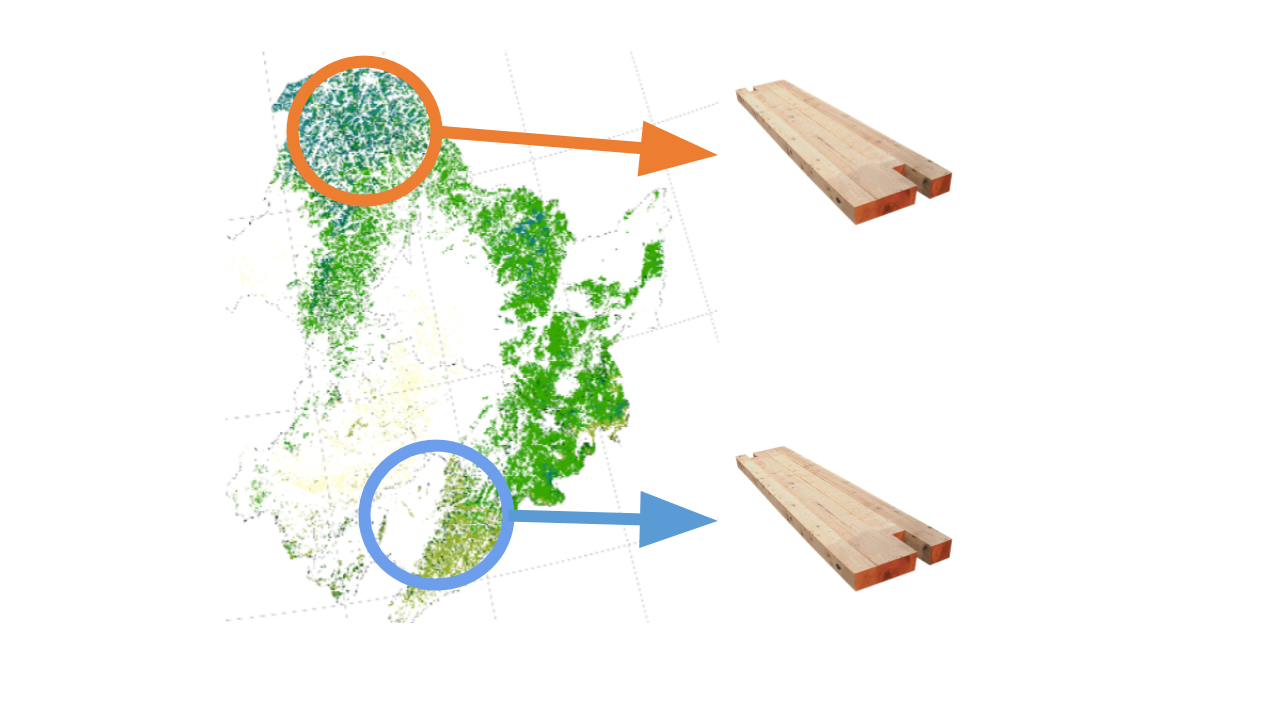
\includegraphics[keepaspectratio,
                              width=\paperwidth]{images/regionalize2.png}
            };
      \end{tikzpicture}
     \note[]{}
\end{frame}
}

{ %%% blank frame
\begin{frame}<article:0>[plain]
   \frametitle{}
      \begin{tikzpicture}[remember picture,overlay]
         \node[at=(current page.center)] {
             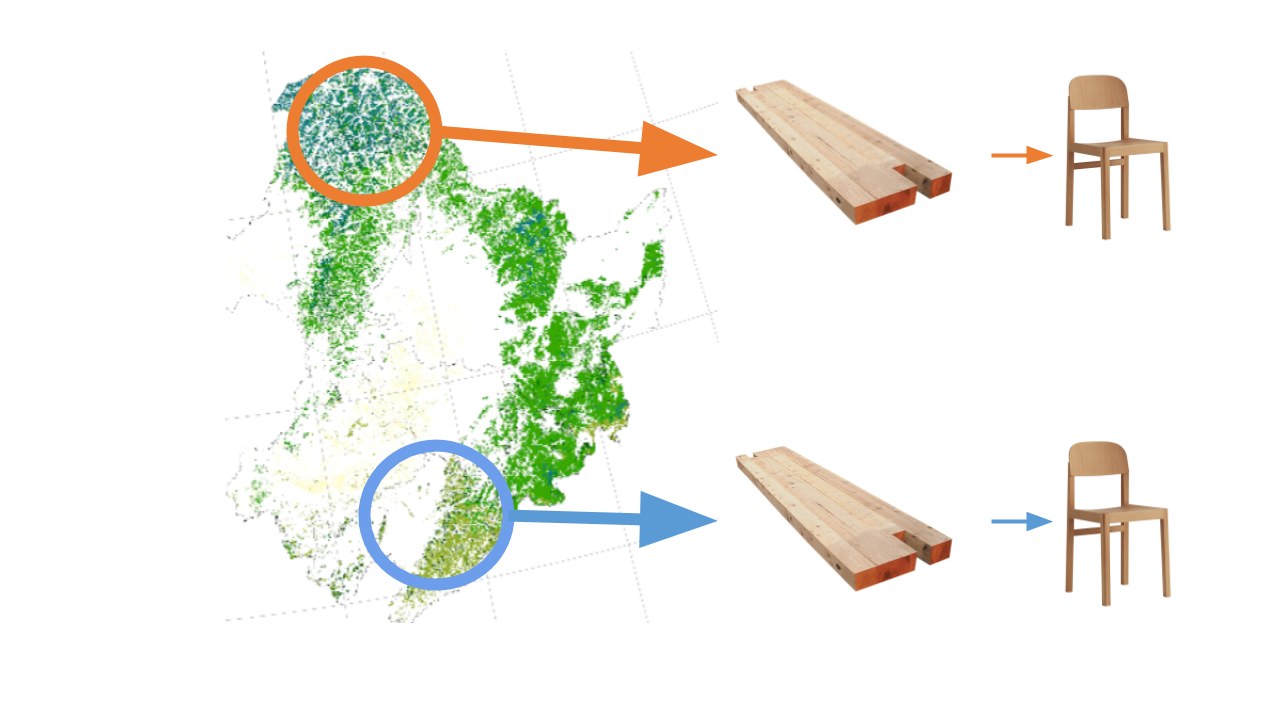
\includegraphics[keepaspectratio,
                              width=\paperwidth]{images/regionalize3.png}
            };
      \end{tikzpicture}
     \note[]{}
\end{frame}
}

{ %%% blank frame
\begin{frame}<article:0>[plain]
   \frametitle{}
      \begin{tikzpicture}[remember picture,overlay]
         \node[at=(current page.center)] {
             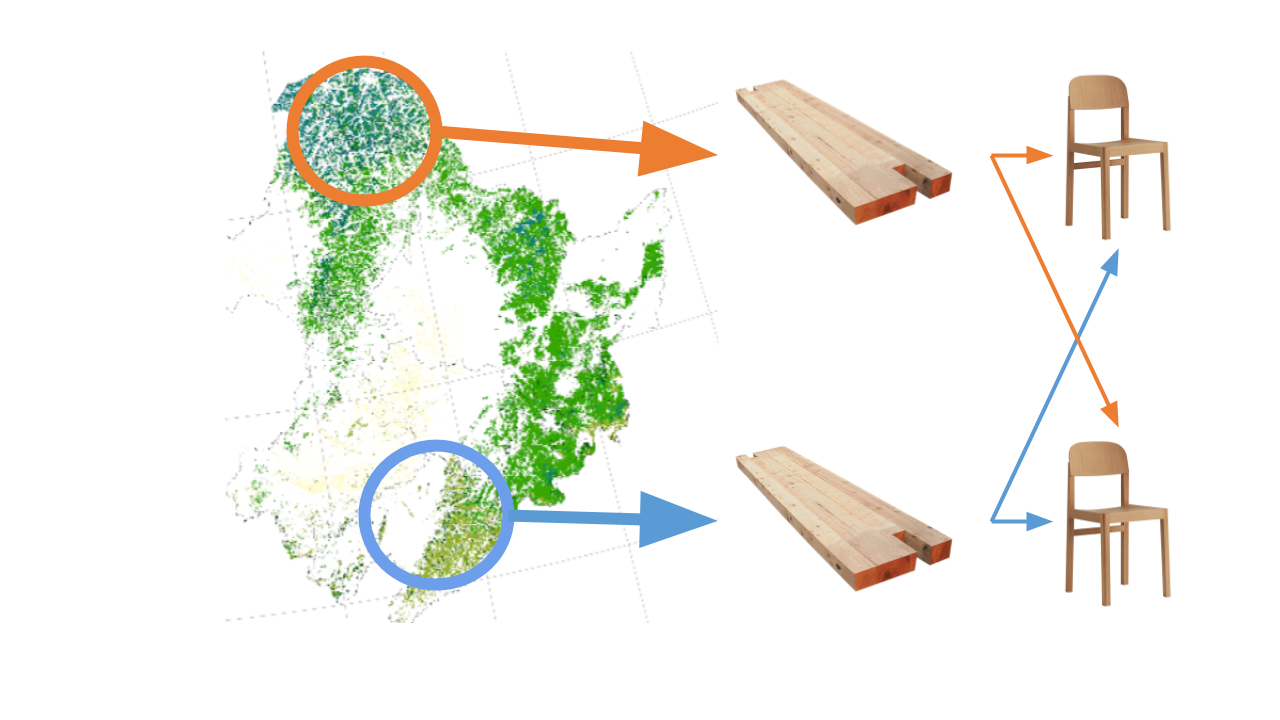
\includegraphics[keepaspectratio,
                              width=\paperwidth]{images/regionalize4.png}
            };
      \end{tikzpicture}
     \note[]{}
\end{frame}
}

{ 
\begin{frame}<article:0>[plain]
   \frametitle{}
      \begin{tikzpicture}[remember picture,overlay]
         \node[at=(current page.center)] {
             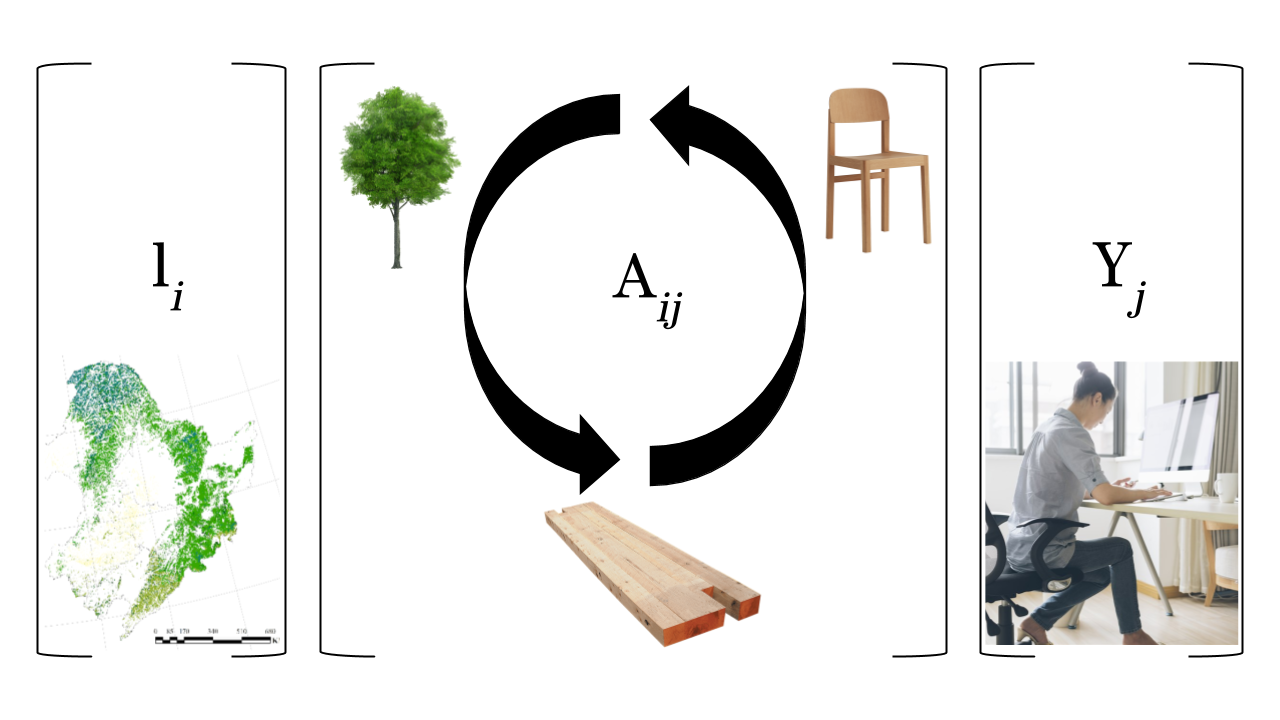
\includegraphics[keepaspectratio,
                              width=\paperwidth]{images/le-mrio-form.png}
            };
      \end{tikzpicture}
     \note[]{}
\end{frame}
}



{ 
\begin{frame}<article:0>[plain]
   \frametitle{}
      \begin{tikzpicture}[remember picture,overlay]
         \node[at=(current page.center)] {
             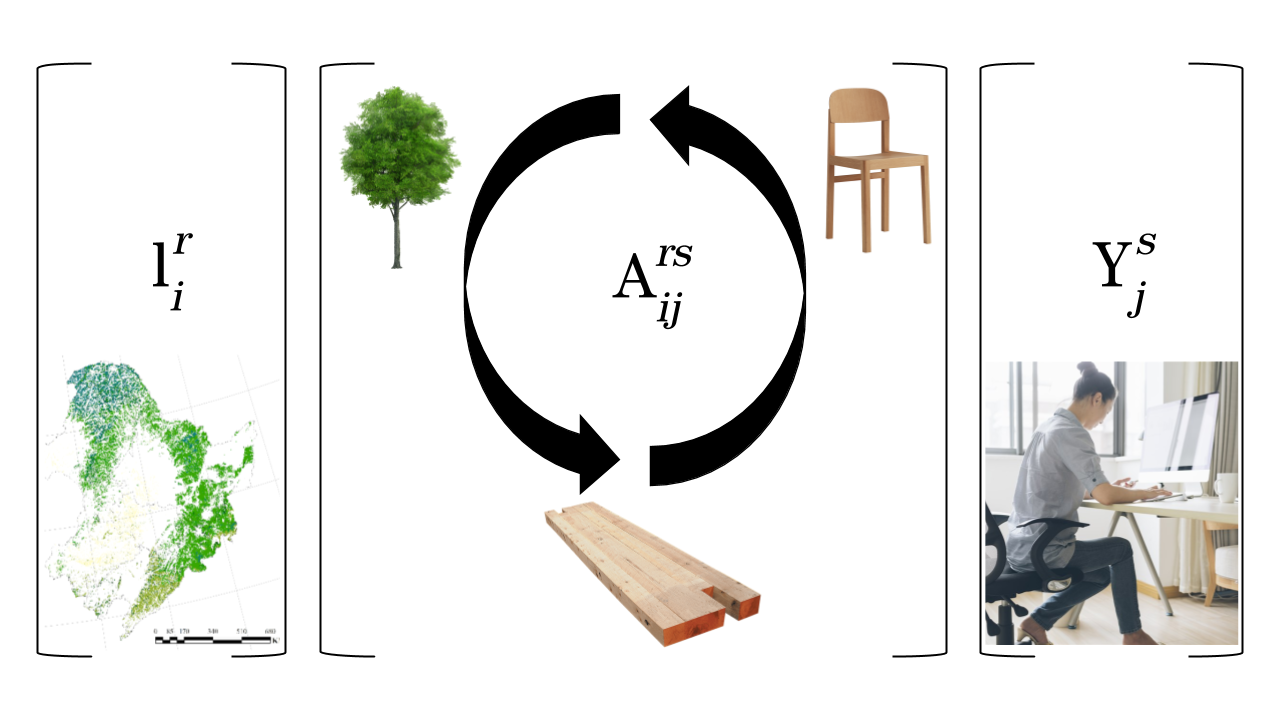
\includegraphics[keepaspectratio,
                              width=\paperwidth]{images/lemrio_rs.png}
            };
      \end{tikzpicture}
     \note[]{}
\end{frame}
}



{
\begin{frame}<article:0>[plain]
   \frametitle{}
      \begin{tikzpicture}[remember picture,overlay]
         \node[at=(current page.center)] {
             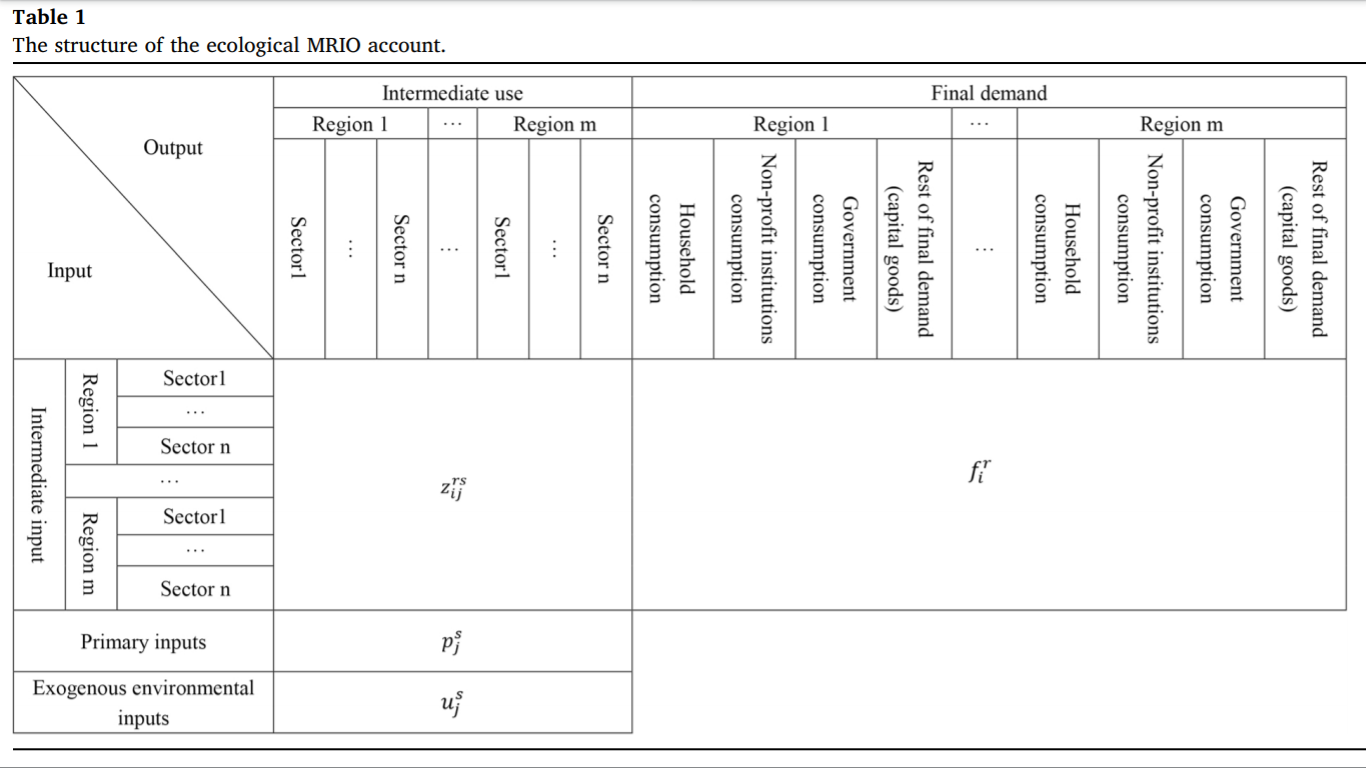
\includegraphics[keepaspectratio,
                              width=\paperwidth]{images/Wu_2018_Table1.png}
            };
      \end{tikzpicture}
     \note[item]{This is why they're called input-output tables}
     \note[item]{Each region has a set of sectors/industries}
     \note[item]{They can receive inputs from within a region}
     \note[item]{They can also recieve input from another region (aka. imports)}
     \note[item]{Final use = Consumption not used to produce another product}
\end{frame}
}



\begin{frame}
  \frametitle{A few EE-MRIO Applications}
  \begin{itemize}
  \item Global carbon emmisions are primarily indirect by developed
  country consumption (23\%) \cite{LIDDLE201871} \pause
  \item 17\% of biodiversity is embodied in food exported to
  high income countries \cite{CHAUDHARY2016195}  \pause
  \item Tropical forest loss in Brazil driven by conversion to soy
  exported primarily to China (48.6\%) and the USA (72.3\%) \cite{Schaffer-Smith2018}
  \end{itemize}
\end{frame}


%% { %%% blank frame
%% \begin{frame}<article:0>[plain]
%%    \frametitle{}
%%       \begin{tikzpicture}[remember picture,overlay]
%%          \node[at=(current page.center)] {
%%              \includegraphics[keepaspectratio,
%%                               width=\paperwidth]{images/}
%%             };
%%       \end{tikzpicture}
%%      \note[]{}
%% \end{frame}
%% }


\section{Global Trade Networks of Forest Landscapes}
 

\begin{frame}
  \frametitle{Global Embodied Landscape Trade Networks}
    \begin{center}
    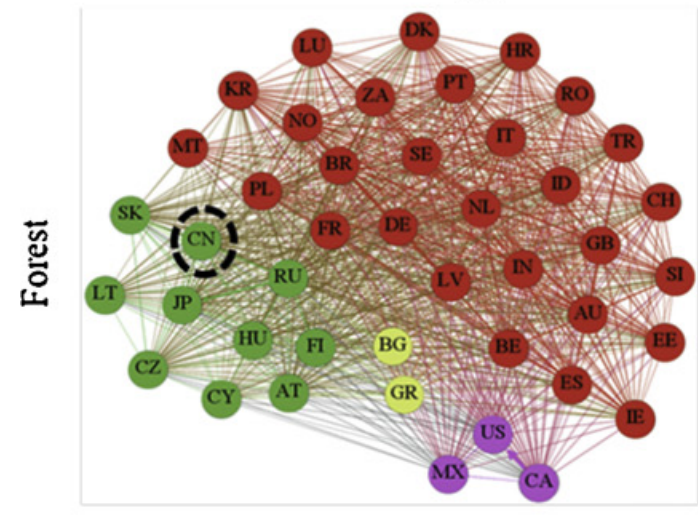
\includegraphics[width=0.2\textwidth]{images/Tian_2019_Fig3_inset_inset.png}  
    \end{center}

\end{frame}


\begin{frame}
  \frametitle{Global Embodied Landscape Trade Networks}
  \begin{center}
  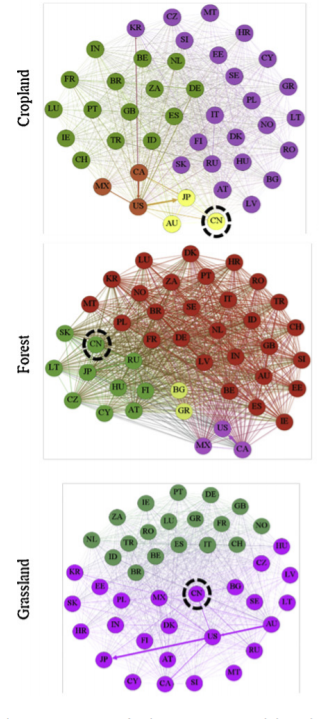
\includegraphics[width=0.2\textwidth]{images/Tian_2019_Fig3_inset.png}
  \end{center}
\end{frame}

\begin{frame}
  \frametitle{Global Embodied Landscape Trade Networks}
  \begin{center}
  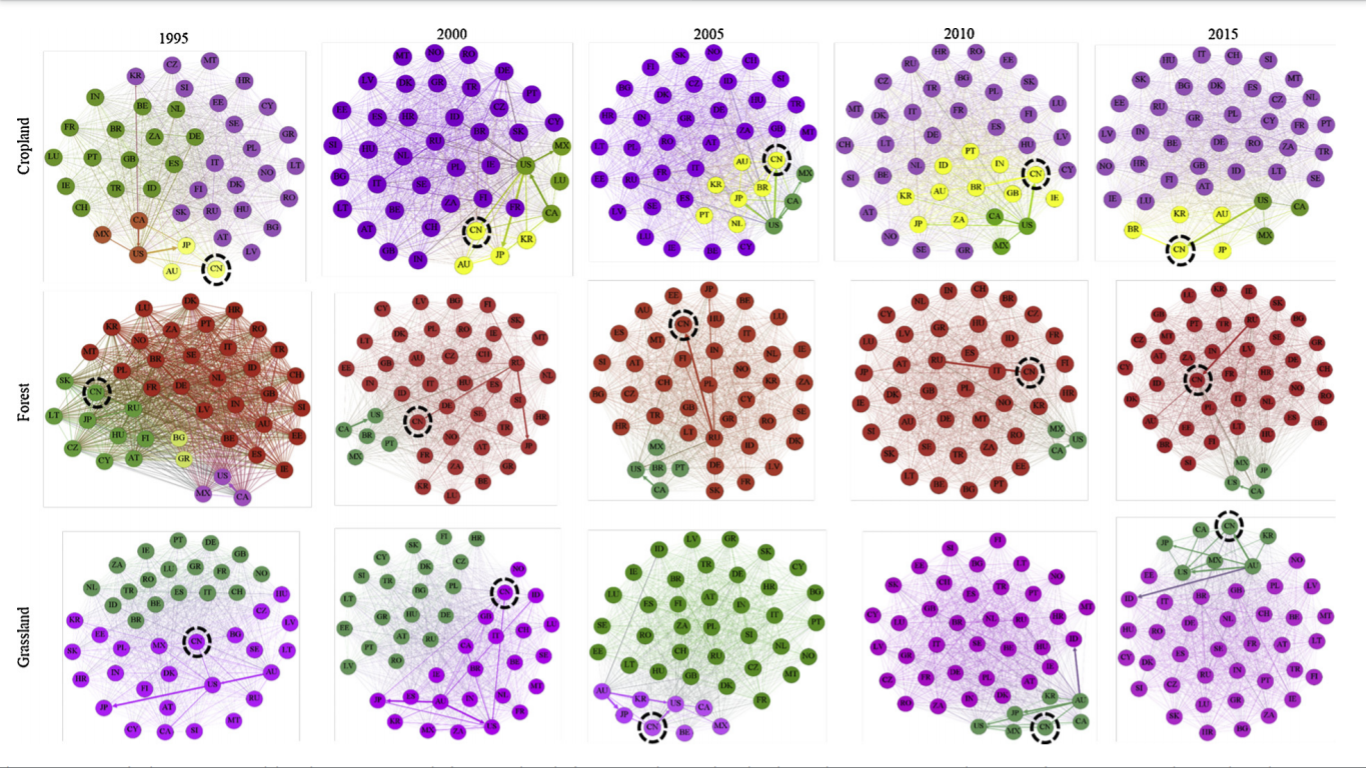
\includegraphics[width=1.0\textwidth]{images/Tian_2019_Fig3.png}
  \end{center}
\end{frame}

{ % all template changes are local to this group.
%%    \setbeamertemplate{navigation symbols}{}
    \begin{frame}<article:0>[plain]
      \frametitle{}
        \begin{tikzpicture}[remember picture,overlay]
            \node[at=(current page.center)] {
                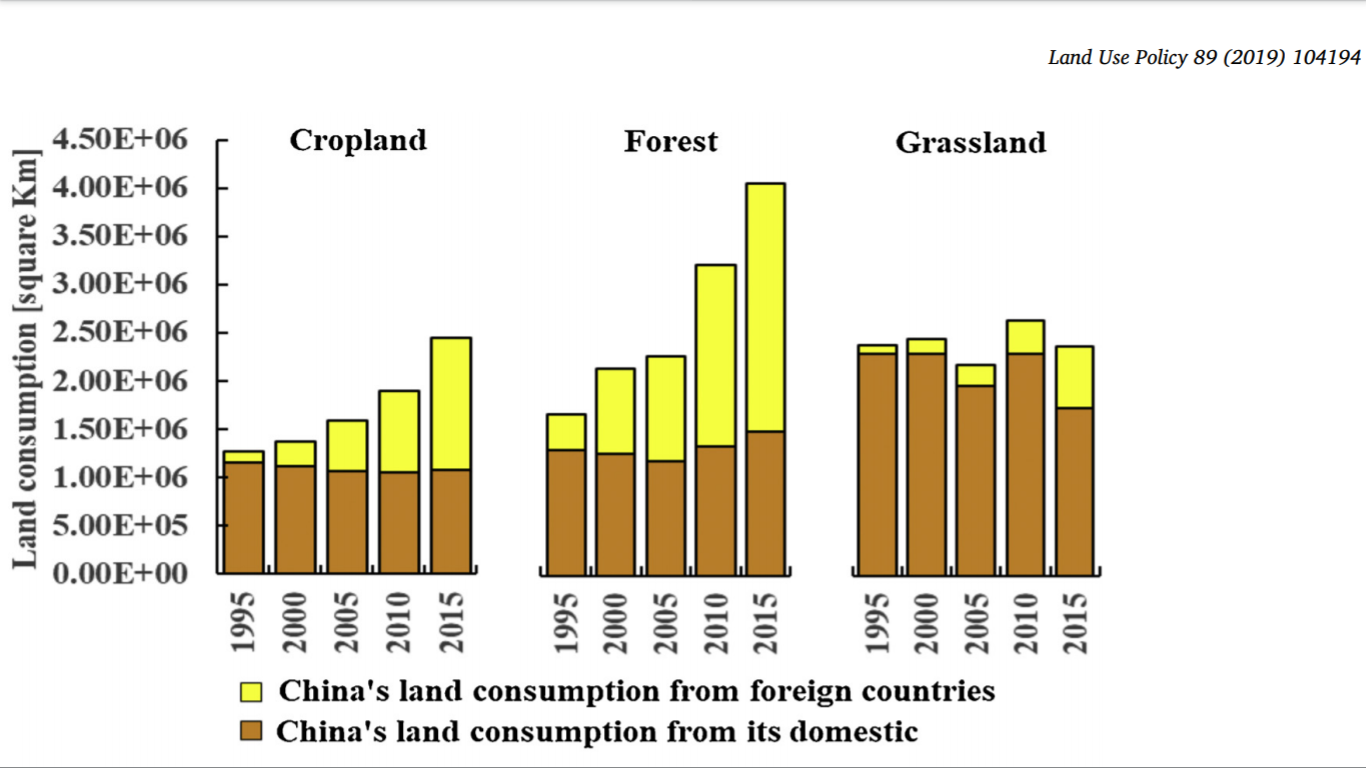
\includegraphics[keepaspectratio,
                                 width=\paperwidth]{images/Tian_2019_Fig1.png}
            };
        \end{tikzpicture}
     \end{frame}
}



{ % all template changes are local to this group.
%%    \setbeamertemplate{navigation symbols}{}
    \begin{frame}<article:0>[plain]
      \frametitle{}
        \begin{tikzpicture}[remember picture,overlay]
            \node[at=(current page.center)] {
                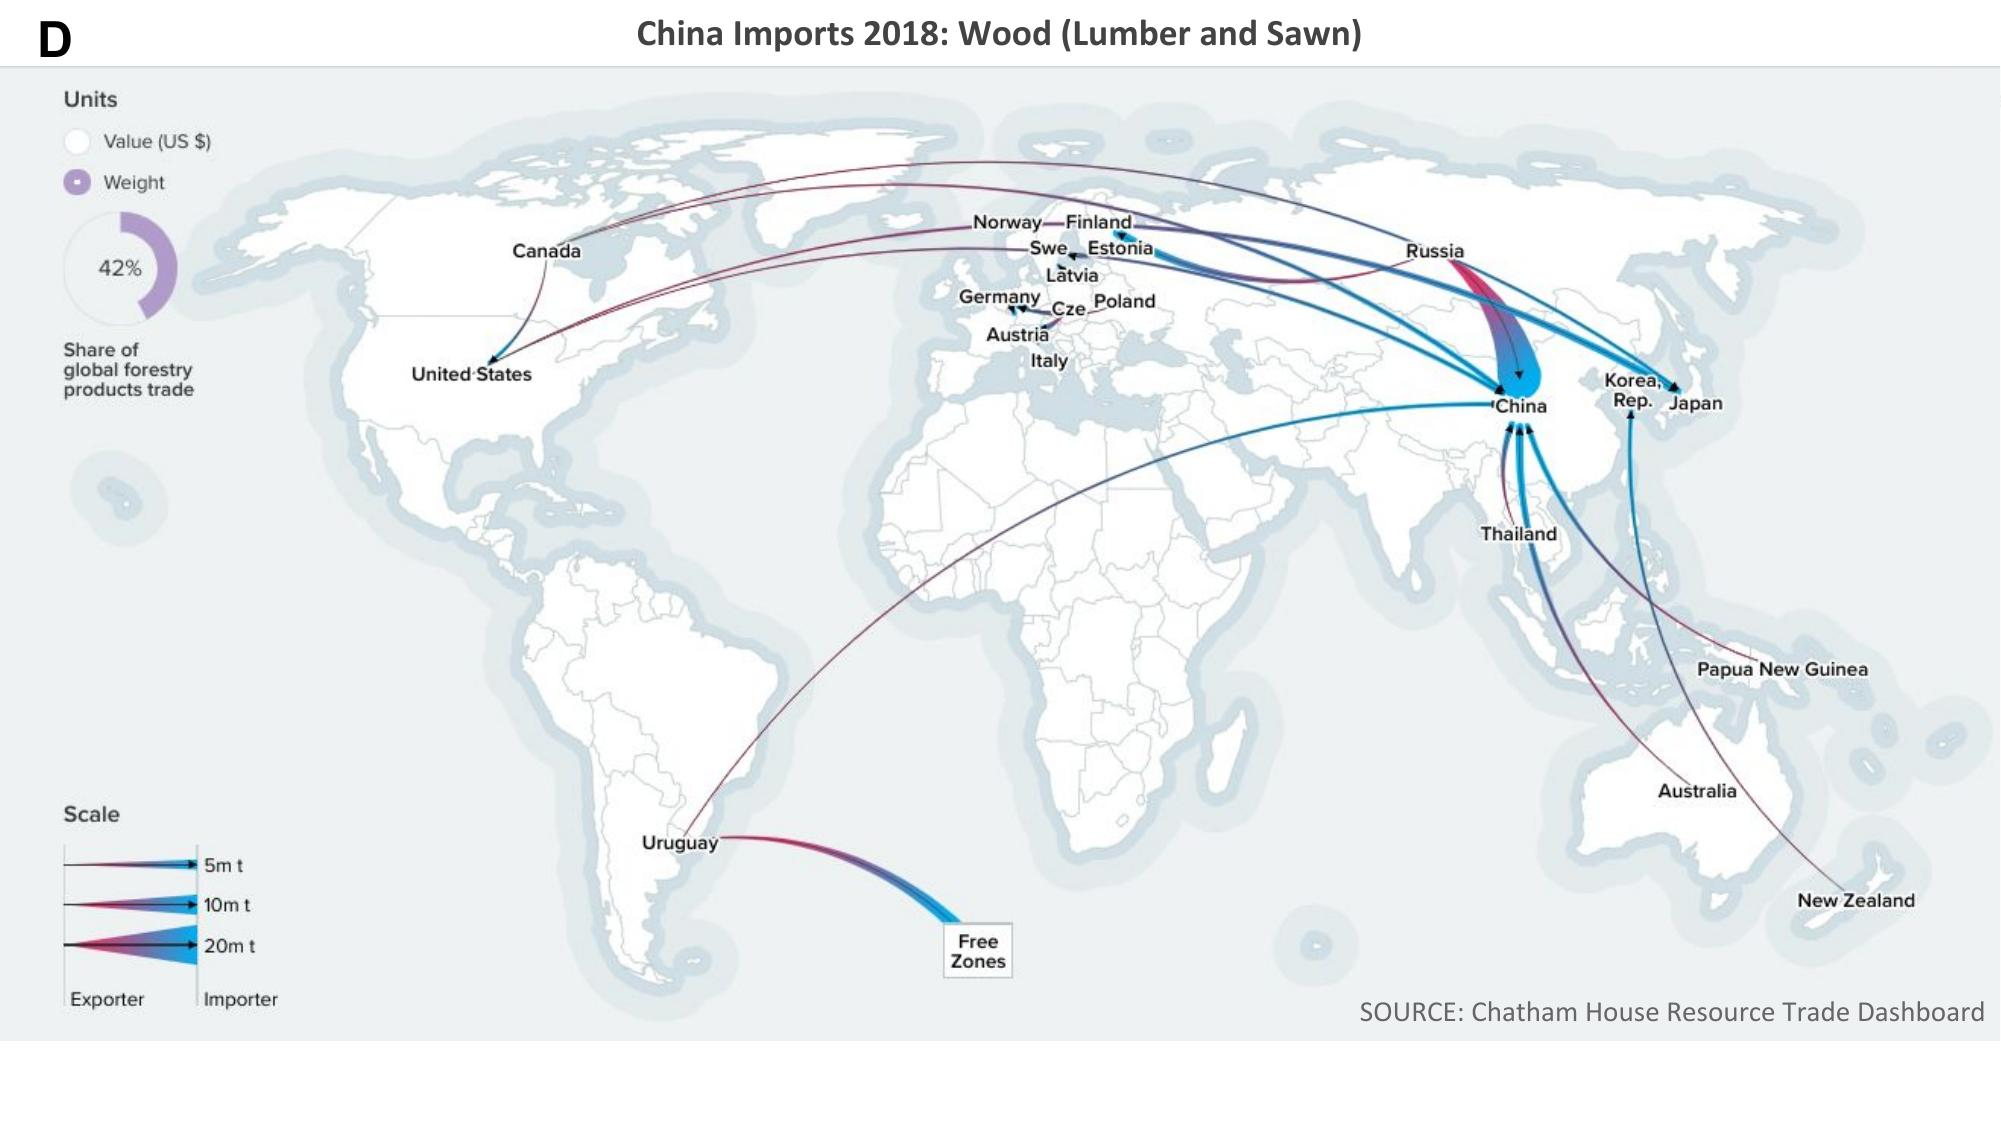
\includegraphics[keepaspectratio,
                                 width=\paperwidth]{images/resourcetrade_network.jpeg}
            };
        \end{tikzpicture}
     \end{frame}
}


{ % all template changes are local to this group.
%%    \setbeamertemplate{navigation symbols}{}
    \begin{frame}<article:0>[plain]
      \frametitle{}
        \begin{tikzpicture}[remember picture,overlay]
            \node[at=(current page.center)] {
                \includegraphics[keepaspectratio,
                                 width=\paperwidth]{images/comtrade_china_imports_wood.jpeg}
            };
        \end{tikzpicture}
     \note[item]{China's imports have been increasing over time}
     \note[item]{Mostly from Russia and USA, lesser Canada and New Zealand}
     \note[item]{Cumulatively, southeast Asian countries rival Russia ($43,621)}
     \end{frame}
}


\section{China's Forest Networks}


{ % all template changes are local to this group.
%%    \setbeamertemplate{navigation symbols}{}
    \begin{frame}<article:0>[plain]
      \frametitle{}
        \begin{tikzpicture}[remember picture,overlay]
            \node[at=(current page.center)] {
                \includegraphics[keepaspectratio,
                                 width=\paperwidth]{images/annual-change-forest-area.png}
            };
        \end{tikzpicture}
        \note[item]{Global forest loss and gain and change}
        \note[item]{Global greening = India(Agriculture) + China(Forests)}
     \end{frame}
}



\begin{frame}
     \frametitle{Redundancy $\sim$ Efficiency}
        \includegraphics[width=\paperwidth]{images/net_info_dynamics.PNG}
\end{frame}

\begin{frame}
  \frametitle{Redundancy $\sim$ Efficiency}
  \begin{center}
  $H = -\sum_{i = 1}^{n} p_i ln(p_i)$
  \end{center}
\end{frame}

\begin{frame}
  \frametitle{Redundancy $\sim$ Efficiency}
  \begin{center}
  $\Psi = -k\sum_{i=1,j=1}^{nn} \frac{T_{ij}}{T_{..}}\ln(\frac{T_{ij}^{2}}{T_{i.}T_{.j}})$
  \end{center}
\end{frame}



{ % all template changes are local to this group.
%%    \setbeamertemplate{navigation symbols}{}
    \begin{frame}<article:0>[plain]
      \frametitle{}
        \begin{tikzpicture}[remember picture,overlay]
             \node[at=(current page.center)] {
                \includegraphics[keepaspectratio,
                                 width=\paperwidth]{images/cn_for_yu/IMG_0226.PNG}
            };
        \end{tikzpicture}
        \note[item]{China's Forests are Diverse}
     \end{frame}
}



{ % all template changes are local to this group.
%%    \setbeamertemplate{navigation symbols}{}
    \begin{frame}<article:0>[plain]
      \frametitle{}
        \begin{tikzpicture}[remember picture,overlay]
            \node[at=(current page.center)] {
                \includegraphics[keepaspectratio,
                                 width=\paperwidth]{images/cn_for_yu/IMG_0227.PNG}
            };
        \end{tikzpicture}

     \end{frame}
}





{ % all template changes are local to this group.
%%    \setbeamertemplate{navigation symbols}{}
    \begin{frame}<article:0>[plain]
      \frametitle{}
        \begin{tikzpicture}[remember picture,overlay]
            \node[at=(current page.center)] {
                \includegraphics[keepaspectratio,
                                 width=\paperwidth]{images/cn_for_yu/IMG_0231.JPG}
            };
        \end{tikzpicture}
        \note[item]{China's Forests are Diverse}
     \end{frame}
}



{ % all template changes are local to this group.
%%    \setbeamertemplate{navigation symbols}{}
    \begin{frame}<article:0>[plain]
      \frametitle{}
        \begin{tikzpicture}[remember picture,overlay]
            \node[at=(current page.center)] {
                \includegraphics[keepaspectratio,
                                 width=\paperwidth]{images/cn_for_yu/IMG_0232.JPG}
            };
        \end{tikzpicture}
        \note[item]{China's Forests are Diverse}
     \end{frame}
}



{ % all template changes are local to this group.
%%    \setbeamertemplate{navigation symbols}{}
    \begin{frame}<article:0>[plain]
      \frametitle{}
        \begin{tikzpicture}[remember picture,overlay]
            \node[at=(current page.center)] {
                \includegraphics[keepaspectratio,
                                 width=\paperwidth]{images/cn_for_yu/IMG_0233.JPG}
            };
        \end{tikzpicture}
        \note[item]{China's Forests are Diverse}
     \end{frame}
}



{ % all template changes are local to this group.
%%    \setbeamertemplate{navigation symbols}{}
    \begin{frame}<article:0>[plain]
      \frametitle{}
        \begin{tikzpicture}[remember picture,overlay]
            \node[at=(current page.center)] {
                \includegraphics[keepaspectratio,
                                 width=\paperwidth]{images/cn_for_yu/IMG_0234.JPG}
            };
        \end{tikzpicture}
        \note[item]{China's Forests are Diverse}
     \end{frame}
}



{ % all template changes are local to this group.
%%    \setbeamertemplate{navigation symbols}{}
    \begin{frame}<article:0>[plain]
      \frametitle{}
        \begin{tikzpicture}[remember picture,overlay]
            \node[at=(current page.center)] {
                \includegraphics[keepaspectratio,
                                 width=\paperwidth]{images/cn_for_yu/IMG_0235.JPG}
            };
        \end{tikzpicture}
        \note[item]{China's Forests are Diverse}
     \end{frame}
}



{ % all template changes are local to this group.
%%    \setbeamertemplate{navigation symbols}{}
    \begin{frame}<article:0>[plain]
      \frametitle{}
        \begin{tikzpicture}[remember picture,overlay]
            \node[at=(current page.center)] {
                \includegraphics[keepaspectratio,
                                 width=\paperwidth]{images/cn_for_yu/IMG_0236.JPG}
            };
        \end{tikzpicture}
        \note[item]{China's Forests are Diverse}
     \end{frame}
}



{ % all template changes are local to this group.
%%    \setbeamertemplate{navigation symbols}{}
    \begin{frame}<article:0>[plain]
      \frametitle{}
        \begin{tikzpicture}[remember picture,overlay]
            \node[at=(current page.center)] {
                \includegraphics[keepaspectratio,
                                 width=\paperwidth]{images/cn_for_yu/IMG_0237.JPG}
            };
        \end{tikzpicture}
        \note[item]{China's Forests are Diverse}
     \end{frame}
}



{ % all template changes are local to this group.
%%    \setbeamertemplate{navigation symbols}{}
    \begin{frame}<article:0>[plain]
      \frametitle{}
        \begin{tikzpicture}[remember picture,overlay]
            \node[at=(current page.center)] {
                \includegraphics[keepaspectratio,
                                 width=\paperwidth]{images/cn_for_yu/IMG_0238.JPG}
            };
        \end{tikzpicture}
        \note[item]{China's Forests are Diverse}
     \end{frame}
}



{ % all template changes are local to this group.
%%    \setbeamertemplate{navigation symbols}{}
    \begin{frame}<article:0>[plain]
      \frametitle{}
        \begin{tikzpicture}[remember picture,overlay]
            \node[at=(current page.center)] {
                \includegraphics[keepaspectratio,
                                 width=\paperwidth]{images/cn_for_yu/IMG_0239.JPG}
            };
        \end{tikzpicture}
        \note[item]{China's Forests are Diverse}
     \end{frame}
}



{ % all template changes are local to this group.
%%    \setbeamertemplate{navigation symbols}{}
    \begin{frame}<article:0>[plain]
      \frametitle{}
        \begin{tikzpicture}[remember picture,overlay]
            \node[at=(current page.center)] {
                \includegraphics[keepaspectratio,
                                 width=\paperwidth]{images/cn_for_yu/IMG_0240.JPG}
            };
        \end{tikzpicture}
        \note[item]{China's Forests are Diverse}
     \end{frame}
}



{ % all template changes are local to this group.
%%    \setbeamertemplate{navigation symbols}{}
    \begin{frame}<article:0>[plain]
      \frametitle{}
        \begin{tikzpicture}[remember picture,overlay]
            \node[at=(current page.center)] {
                \includegraphics[keepaspectratio,
                                 width=\paperwidth]{images/cn_for_yu/IMG_0241.JPG}
            };
        \end{tikzpicture}
        \note[item]{China's Forests are Diverse}
     \end{frame}
}



{ % all template changes are local to this group.
%%    \setbeamertemplate{navigation symbols}{}
    \begin{frame}<article:0>[plain]
      \frametitle{}
        \begin{tikzpicture}[remember picture,overlay]
            \node[at=(current page.center)] {
                \includegraphics[keepaspectratio,
                                 width=\paperwidth]{images/cn_for_yu/IMG_0242.JPG}
            };
        \end{tikzpicture}
        \note[item]{China's Forests are Diverse}
     \end{frame}
}



{ % all template changes are local to this group.
%%    \setbeamertemplate{navigation symbols}{}
    \begin{frame}<article:0>[plain]
      \frametitle{}
        \begin{tikzpicture}[remember picture,overlay]
            \node[at=(current page.center)] {
                \includegraphics[keepaspectratio,
                                 width=\paperwidth]{images/cn_for_yu/IMG_0243.JPG}
            };
        \end{tikzpicture}
        \note[item]{China's Forests are Diverse}
     \end{frame}
}



{ % all template changes are local to this group.
%%    \setbeamertemplate{navigation symbols}{}
    \begin{frame}<article:0>[plain]
      \frametitle{}
        \begin{tikzpicture}[remember picture,overlay]
            \node[at=(current page.center)] {
                \includegraphics[keepaspectratio,
                                 width=\paperwidth]{images/cn_for_yu/IMG_0244.JPG}
            };
        \end{tikzpicture}
        \note[item]{China's Forests are Diverse}
     \end{frame}
}



{ % all template changes are local to this group.
%%    \setbeamertemplate{navigation symbols}{}
    \begin{frame}<article:0>[plain]
      \frametitle{}
        \begin{tikzpicture}[remember picture,overlay]
            \node[at=(current page.center)] {
                \includegraphics[keepaspectratio,
                                 width=\paperwidth]{images/cn_for_yu/IMG_0245.JPG}
            };
        \end{tikzpicture}
        \note[item]{China's Forests are Diverse}
     \end{frame}
}



{ % all template changes are local to this group.
%%    \setbeamertemplate{navigation symbols}{}
    \begin{frame}<article:0>[plain]
      \frametitle{}
        \begin{tikzpicture}[remember picture,overlay]
            \node[at=(current page.center)] {
                \includegraphics[keepaspectratio,
                                 width=\paperwidth]{images/cn_for_yu/IMG_0246.JPG}
            };
        \end{tikzpicture}
        \note[item]{China's Forests are Diverse}
     \end{frame}
}



{ % all template changes are local to this group.
%%    \setbeamertemplate{navigation symbols}{}
    \begin{frame}<article:0>[plain]
      \frametitle{}
        \begin{tikzpicture}[remember picture,overlay]
            \node[at=(current page.center)] {
                \includegraphics[keepaspectratio,
                                 width=\paperwidth]{images/cn_for_yu/IMG_0247.JPG}
            };
        \end{tikzpicture}
        \note[item]{China's Forests are Diverse}
     \end{frame}
}



\begin{frame}
  \frametitle{China's Forest Networks: Global}
\end{frame}


\begin{frame}
  \frametitle{China's Forest Networks: Domestic/Local}
\end{frame}

%%   - Local Scale
%% 	- Landscape = Chen 2019
%% 	- Resilience Analysis of China's Forest LE-MRIO

\section{Conclusions}

\begin{frame}
  \frametitle{Conclusions}

\begin{itemize}
\item Localization of resource consumption increases modularity
\item This is line with recent observations of the benefits of
empowering local communities for forest restoration
\item 
\end{itemize}

\end{frame}

\section{Future Work}

\begin{frame}
  \frametitle{Future Work}
\end{frame}


\begin{frame}
  \frametitle{Future Work}
\begin{columns}
\begin{column}{0.5\textwidth}
    \begin{center}
     \includegraphics[width=0.86\textwidth]{images/moran_2020_1.png}
     \end{center}
\end{column}
\begin{column}{0.5\textwidth}  %%<--- here
    \begin{center}
     \includegraphics[width=1.0\textwidth]{images/moran_2020_2.png}
     \end{center}
\end{column}
\end{columns}
\end{frame}

\begin{frame}
  \frametitle{Cool Projects to Check Out}
  \begin{itemize}
  \item \url{www.globalcanopy.org} - Financial Sector Transparency
  \item \url{www.fineprint.global} - Product Sourcing Analysis 
  \item \url{trase.earth} - Stakeholder and Investor Information
  \end{itemize}
\end{frame}





\begin{frame}
  \frametitle{Acknowledgements}
\end{frame}



{ % all template changes are local to this group.
%%    \setbeamertemplate{navigation symbols}{}
    \begin{frame}<article:0>[plain]
      \frametitle{}
        \begin{tikzpicture}[remember picture,overlay]
            \node[at=(current page.center)] {
                \includegraphics[keepaspectratio,
                                 width=\paperwidth]{images/CNF/IMG_0199.JPG}
            };
        \end{tikzpicture}
        \note[item]{Questions, comments?}
     \end{frame}
}

\begin{frame}
  \cite{Burgess2012}    
  \cite{Caggiani2014}
  \cite{Carvalho2019AdaptationSystems}
  \cite{Schaffer-Smith2018NetworkTrade}
\end{frame}


\begin{frame}[allowframebreaks]
  \frametitle{References}
  \tiny \bibliography{biblio.bib}
  \bibliographystyle{abbrv}
\end{frame}


\end{document}
